\documentclass[12pt,a4paper]{report} %Formato y formas principales
\usepackage[spanish]{babel} %Establecer idioma
\usepackage{graphicx} %Para añadir imágenes
\usepackage{fancyhdr} %Para establecer mi propio encabezado y pie de página
\usepackage[left=3cm,right=3cm,top=2.5cm,bottom=2.5cm,headsep=1cm]{geometry} % Mis márgenes
%\setlength{\headheight}{14.0pt} %Ajusta el tamaño del encabezado
%\linespread{1.5} % Espaciado de 1.5 (1 es el espaciado estándar)
%\setlength{\parindent}{0pt} %Ajusta la sangría a 0 para que no haya
\usepackage{amsmath} %Para ecuaciones\usepackage{amsmath}
\usepackage{amssymb} % Paquete para cargar la fuente \mathbb
\usepackage{amsthm}
\usepackage{mathtools}
\usepackage{multicol}
%\usepackage{refcheck} %Para que aparezca el nombre que le doy a la referencia
\usepackage{comment} %Para comentar varias lineas
\usepackage{lipsum} %Para hacer textos de ejemplo para pruebas
\usepackage{bm} % Agrega esta línea en el preámbulo del documento
\usepackage{enumitem}
\usepackage{xcolor}
\usepackage{matlab-prettifier}
\usepackage{empheq}
\decimalpoint

\newtheorem{theorem}{Teorema}[chapter]
\newtheorem{definicion}{Definición}[chapter] % Declaración del nuevo entorno "definicion"


\usepackage{caption} %Para crear mi formato "boldformat" que pone lo primero en negrita
\DeclareCaptionFormat{boldformat}{\textbf{#1} #2 #3}
\captionsetup[figure]{format=boldformat} %Le asigno el formato al de las figuras

\usepackage{hyperref} %Para que haya hipervínculos
\hypersetup{
	colorlinks=true, %Para que los hipervínculos sean de color y no con caja roja
	linkcolor=blue,
	urlcolor=black,
	citecolor=blue,
}

\makeatletter %Mi propio comando para establecer las referencias de figuras y ecuaciones
\newcommand{\fref}[1]{\hyperref[#1]{\textcolor{blue}{\textit{Fig.~\ref*{#1}}}}}
\newcommand{\eref}[1]{\hyperref[#1]{\textcolor{blue}{\textit{(\ref*{#1})}}}}
\newcommand{\tr}{\operatorname{\textrm{tr}}}
\makeatother

\usepackage{makeidx} %Para hacer el indice
\makeindex
\usepackage{tocloft} %Para configurar el índice
\renewcommand{\cftchapleader}{\cftdotfill{\cftdotsep}} %Línea puntos índice
\setlength{\cftbeforetoctitleskip}{-1cm} % Ajusta el margen superior del índice

%\usepackage[T1]{fontenc} %Para cambiar la letra y el tamaño
%\usepackage[scaled]{uarial}
%\renewcommand*\familydefault{\sfdefault}


\usepackage{titlesec} %Para cambiar mi formato de chapter
\titleformat{\chapter}[display]
{\normalfont\huge\bfseries}{\chaptertitlename\ \thechapter}{20pt}{\LARGE}
\titlespacing*{\chapter}{0pt}{-1.5cm}{40pt}

\pagestyle{fancy}
\fancyhf{}
\fancyhead[L]{\fontsize{12}{14}\selectfont\leftmark}  % Número de página a 
\fancyhead[R]{\fontsize{12}{14}\selectfont\thepage}  % Número de página 
\fancyfoot[R]{\fontsize{12}{14}\selectfont Sevilla, Julio de 2023}  



\begin{document}
	
	\begin{titlepage}
		\centering
		\hspace*{-1.5cm}\begin{tabular}{@{}l@{}}
			\includegraphics[width=3cm]{b.png} % Logo 1 (esquina superior izquierda)
		\end{tabular}
		\hfill
		\begin{tabular}{c}
			\LARGE\textbf{Universidad de Sevilla} \\ [0.5cm] % Nombre de la universidad
			\LARGE\textbf{Escuela Politécnica Superior} % Otra frase dentro de la misma caja
		\end{tabular}%
		\hfill
		\begin{tabular}{@{}r@{}}
			\includegraphics[width=3cm]{a.png} % Logo 2 (esquina superior derecha)
		\end{tabular}\hspace*{-1.5cm}
		
		\vspace{1.5cm}
		
		\begin{center}
			\Large\textmd{Trabajo Fin de Grado} \\ [0.2cm] % Título 
			\Large\textmd{Ingeniería Electrónica Industrial}
		\end{center}
		
		\vspace{2cm}
		
		\begin{center}
			\LARGE\textsl{La caracterización integral de las semiaplicaciones de Poincaré y su aplicación a circuitos electrónicos: El Memristor}
		\end{center}
		
		\vspace{7cm}
		
		\raggedright
		\large\textbf{Autor:} Sergio R. Durán Martín \\ [0.5cm]
		\large\textbf{Tutor:} Dr. Victoriano Carmona Centeno \\ [0.5cm]
		\large\textbf{Departamento:} Matemática Aplicada II
	\end{titlepage}
	
	\clearpage
	\null
	\thispagestyle{empty}
	\newpage

\begin{center}
	\LARGE\textbf{Resumen}
\end{center}
\begin{minipage}{\textwidth}
	\lipsum[1]
	
	\vspace{0.5cm}
	\noindent \textbf{Palabras clave:} robótica educativa, robot modular, STM32, FreeRTOS, interfaz gráfica, impresión 3D.
\end{minipage}

\vspace{1cm}

\begin{center}
	\LARGE\textbf{Abstract}
\end{center}
\begin{minipage}{\textwidth}
	\lipsum[2]
	
	\vspace{0.5cm}
	\noindent \textbf{Keywords:} educational robotics, modular robot, STM32, FreeRTOS, graphic interface, 3D printing.
\end{minipage}
\newpage
	
\tableofcontents
	\chapter{Introducción}
	Contenido del capítulo de introducción. Contenido del capítulo 1.
	
	\chapter{Descripción del Circuito}
	\noindent El circuito que se ha estudiado es un oscilador con resistencia negativa al que se le ha añadido un componente muy interesante y que está siendo muy estudiado en estos últimos tiempos, el memristor, ver \fref{fig:-RLCM}.
	
	\begin{figure}[h]
		\centering
		\includegraphics[width=0.7\textwidth]{-RLCM.png}
		\caption{Oscilador RLC con R negativa y Memristor.}
		\label{fig:-RLCM}
	\end{figure}
	
	Como se puede ver no existe una fuente de señal en el circuito y esto se debe a que el análisis hecho busca encontrar una oscilación periódica tan solo proporcionando condiciones iniciales a la bobina y el condensador, esto gracias al comportamiento de la resistencia negativa y del memristor los cuales se especifican mas adelante.
	
	\vspace{0.5cm}La forma de imponer las condiciones iniciales serían las clásicas, usando fuentes de intensidad en serie y tensión en paralelo con interruptores que se abren en \\$t\,=\,0(s)$ para la bobina y el condensador respectivamente.
	
	\newpage
	\section{Resistencia negativa}
	\noindent Uno de los componentes del circuito es la resistencia negativa la cual se puede construir con lo que se llama un \emph{Convertidor de Impedancia Negativa (NIC)}. Un NIC es un circuito activo, es decir, en lugar de disipar energía como una resistencia convencional, puede proporcionar energía a un circuito, ver \fref{fig:NIC}. En términos prácticos, un NIC puede ser utilizado para compensar la resistencia de carga de un sistema, mejorar la eficiencia de la transferencia de energía o realizar otras funciones específicas en circuitos eléctricos o electrónicos. En los circuitos osciladores, el NIC desempeña un papel importante en el mantenimiento, estabilización, frecuencia y calidad de la oscilación.
	 
	\begin{figure}[h]
		\centering
		\includegraphics[width=0.65\textwidth]{NIC_B.jpg}
		\caption{Convertidor de Impedancia Negativa de -1000 Ohmios.}
		\label{fig:NIC}
	\end{figure}
	
	\newpage
	
	\noindent Una de las maneras de realizarlo es usando un amplificador operacional y 3 resistencias en la configuración que se ve en la \fref{fig:NIC} de esta manera si elegimos las resistencias $R_2=R_3$ la resistencia $R_1$ es la que determinaría el valor de resistencia negativa, esta es la explicación:
	
	\begin{center}
	\begin{multicols}{2}
		\centering
		\includegraphics[width=\columnwidth]{demotracion_NIC.png}
		\captionof{figure}{Parámetros circuito NIC.}
		\label{fig:Param_NIC}
	
		\columnbreak
		
		Consideraciones para el cálculo del circuito de la \fref{fig:Param_NIC} con Amplificadores Operacionales:\\
		\begin{equation}
			V_+\,=\,V_-.
			\label{eq:NIC1}
		\end{equation}
		\begin{equation}
			I_+\,=\,I_-\,=\,0\,(A).
			\label{eq:NIC2}
		\end{equation}
	\end{multicols}
	\end{center}
	
	Si observamos la ecuación \eref{eq:NIC1} se puede ver que la tensión $V_S$ cae sobre la resistencia $R_1$ y se puede relacionar con la tensión de salida $V_O$ mediante un divisor de tensión:
	
	\begin{equation}
		V_S\,=\,V_O\,\frac{R_1}{R_1 + R_2}\:\longrightarrow\:V_O\,=\,V_S\,\frac{R_1 + R_2}{R_1}.
		\label{eq:NIC3}
	\end{equation}\smallskip
	
	Teniendo en cuenta la ecuación \eref{eq:NIC2} se puede ver que la intensidad $I(V_S)$ es la misma que pasa por la resistencia $R_3$, por ello se puede deducir:
	
	\begin{equation}
		I(V_S)\,=\,\frac{V_S - V_O}{R_3}.
		\label{eq:NIC4}
	\end{equation}\smallskip
	
	Sustituyendo la ecuación \eref{eq:NIC3} en \eref{eq:NIC4} y trabajando la expresión para obtener la relacion tensión-intensidad llegamos a:
	
	\begin{equation}
		I(V_S)\,=V_S\,\frac{-R_2}{R_1 \, R_3}.
		\label{eq:NIC5}
	\end{equation}\smallskip
	
	Si dividimos la tensión $V_S$ entre la intensidad $I(V_S)$ (ecuación \eref{eq:NIC5}) para obtener la impedancia de entrada del circuito:
	
	\begin{equation}
		\frac{V_S}{I(V_S)}\,=\,Z_{IN}\,=\,\frac{V_S}{V_S\,\frac{-R_2}{R_1 \, R_3}}\,=\,-R_1\,\frac{R_3}{R_2}.
		\label{eq:NIC6}
	\end{equation}\smallskip
	
	Si elegimos las resistencias $R_3\,=\,R_2$ en la ecuación \eref{eq:NIC6} obtenemos:
	
	\begin{equation}
		Z_{IN}\,=\,-R_1.
		\label{eq:NIC7}
	\end{equation}\smallskip
	
	\newpage
	\section{Memristor}
	\noindent El componente más interesante de este circuito es el Memristor, teorizado por el científico Leon Chua en 1971, ver \cite{chuamissing1971}. Este elemento trata de llenar el vacío que existía en las relaciones entre las cuatro variables básicas en teoría de circuitos: voltaje \textbf{\textit{v}}, intensidad \textbf{\textit{i}}, carga eléctrica \textbf{\textit{q}} y flujo magnético \textit{$\bm{\varphi}$}. En concreto el memristor relaciona la carga eléctrica con el flujo magnético de la siguiente manera, ver \cite{chuaoscillator2008}:
	
	\begin{equation}
		\varphi\,=\,\varphi(q), \qquad q\,=\,q(\varphi).
		\label{eq:flujocarga}
	\end{equation}\smallskip
	
	Sabiendo la relación del voltaje y la intensidad respecto a la carga y al flujo en el tiempo:

	\begin{equation}
		v(t)\,=\,\frac{d\varphi}{dt}, \qquad i(t)\,=\,\frac{dq}{dt}.
		\label{eq:dvdi}
	\end{equation}
			
	\begin{equation}
		\varphi(t)\,=\,\int_{-\infty}^{t}v(\tau)d\tau, \qquad q(t)\,=\,\int_{-\infty}^{t}i(\tau)d\tau.
		\label{eq:flujocargaintegral}
	\end{equation}\smallskip
	
	Derivando la ecuación \eref{eq:flujocarga} respecto al tiempo, y aplicando la regla de la cadena:
	
	\begin{equation}
		\frac{d\varphi}{dt}\,=\,\frac{d\varphi(q)\,dq}{dq\,dt}, \qquad \frac{dq}{dt}\,=\,\frac{dq(\varphi)\,d\varphi}{d\varphi\,dt}.
		\label{eq:vym}
	\end{equation}\smallskip
	
	Sustituyendo las relación de la ecuación \eref{eq:dvdi} en la ecuación \eref{eq:vym}:
	
	\begin{equation}
		v(t)\,=\,\frac{d\varphi(q)}{dq}i(t), \qquad i(t)\,=\,\frac{dq(\varphi)}{d\varphi}v(t).
		\label{eq:vym2}
	\end{equation}\smallskip
	
	Las dos relaciones de carga y flujo que quedan en la ecuación \eref{eq:vym2} son los que se denominan \textbf{\textit{Memristancia M(q)}} y \textbf{\textit{Memductancia W($\bm{\varphi}$)}}: 
	
	\begin{equation}
		M(q)\,=\,\frac{d\varphi(q)}{dq}, \qquad W(\varphi)\,=\,\frac{dq(\varphi)}{d\varphi}.
		\label{eq:myw}
	\end{equation}\smallskip
	
	Finalmente se presentan dos tipos de expresiones:
	
	\begin{equation}
		\textit{Memristor controlado por carga} \, \rightarrow \, v(t)\,=\,M(q)\,i(t).
		\label{eq:cc}
	\end{equation}\smallskip
	\begin{equation}
		\textit{Memristor controlado por flujo} \, \rightarrow \, i(t)\,=\,W(\varphi)\,v(t).
		\label{eq:fc}
	\end{equation}\smallskip

	
	
	\newpage
	
	\noindent El segundo acontecimiento más importante en relación al memristor fue en 2008 cuando en los laboratorios de HP se fabricó un componente cuyo comportamiento era muy parecido al funcionamiento que afirmaba Chua, debía de tener el memristor. En un inicio al componente que HP creó en 2005 le dieron el nombre de \textit{Crossbar Latch}, no sería hasta 2008 que se percataron de la similitud de funcionaminto con el memristor de Chua. La construcción es secilla, se trata de dos capas, una de dioxido de titanio puro y otra de dioxido de titanio deficiente de átomos de oxígeno, ambas envueltas por dos electrodos de platino \fref{fig:mem1}.\textit{\textcolor{red}{Repasar este párrafo, la frase de "debía tener..." quitar}}
	
	\begin{figure}[h]
		\centering
		\includegraphics[width=0.75\textwidth]{mem1.jpg}
		\caption{Costruccion del memristor de HP. Ver \cite{williams}.}
		\label{fig:mem1}
	\end{figure}
	
	El óxido de titanio tiene una serie de características que lo hacen un material muy interesante en esta aplicación:
	\begin{enumerate}
		\item Resistencia variable: La resistencia eléctrica del dióxido de titanio cuando está dopado puede cambiar en repuesta de la aplicación de una corriente o un campo eléctrico. Lo cual nos permite no tan solo guardar 1 o 0 si no un rango de valores dentro de unos límites de operación (memorias ReRAM).
		\item No volatilidad: El óxido de titanio puede mantener su estado de resistencia incluso cuando se retira la corriente eléctrica que lo atraviesa. Esto significa que puede retener información y mantener su estado de resistencia sin requerir energía continua.
		\item Cambios rápidos de resistencia:  Esta propiedad permite operaciones de escritura y lectura rápidas en el memristor, lo que es crucial para su uso en aplicaciones de almacenamiento y procesamiento de datos.
		\item Baja potencia y tamaño compacto
	\end{enumerate}
	\newpage
	
	La fórmula que se propone en \cite{HP} para modelar el comportamiento de este dispositivo es:
	
	\begin{equation}
		v(t)\,=\,\left(R_{ON}\,\frac{w(t)}{D}+R_{OFF}\left(1-\frac{w(t)}{D}\right)\right)i(t),
		\label{eq:hp1}
	\end{equation}
	
	\begin{equation}
		\frac{dw(t)}{dt}\,=\,\mu_V\,\frac{R_{ON}}{D}\,q(t).
		\label{eq:hp2}
	\end{equation}\smallskip
	
	Integrando la ecuación \eref{eq:hp2} e insertándola en \eref{eq:hp1} teniendo en cuenta que el valor de resistencia  $R_{ON} \ll R_{OFF}$: 
	
	\begin{equation}
		w(t)\,=\,\mu_V\,\frac{R_{ON}}{D}\,i(t),
		\label{eq:hp3}
	\end{equation}\smallskip
	\begin{equation}
		M(q)\,=\,R_{OFF}\,\left(1-\,\frac{\mu_V\,R_{ON}}{D^2}\,q(t)\right).
		\label{eq:hp4}
	\end{equation}\smallskip
	
	\begin{figure}[h]
		\centering
		\includegraphics[width=1\textwidth]{schmem.jpg}
		\caption{Esquema del memristor de HP. Ver \cite{2021}.}
		\label{fig:2021}
	\end{figure}\smallskip
	
	Los parámetros que aparecen en las ecuaciones anteriores y que describen el funcionamiento del componente son:
	
	\begin{enumerate}
		\item $R_{ON}$: Resistencia en el estado ON, valor mínimo. Es constante.
		\item $R_{OFF}$: Resistencia en el estado OFF, valor máximo. Es constante.
		\item $\mu_V$: Mobilidad iónica de arrastre promedio. Es constante.
		\item $w$: Ancho de la zona dopada, no es constante, depende de la excitación.
		\item $D$: Ancho total de la lamina de oxido de titanio. Es constante.
	\end{enumerate}
	\newpage
	
	El funcionamiento es el siguiente, entre los dos electrodos de platino tenemos una capa de dióxido de titanio puro $TiO_2$ que actúa como dieléctrico y otra de dióxido de titanio con vacantes de oxígeno $TiO_{2-x}$ que actúa como conductor ya que en estas vacantes están cargadas positivamente (ver \fref{fig:mem1}), ya que al faltar átomos de oxígeno se están perdiendo también sus electrones de valencia asociados, generando así que el compuesto necesite atraer electrones a dichas vacantes para así mantenerse eléctricamente estable.Cuando un voltaje positivo se aplica al electrodo superior las vacantes de oxígeno de la zona dopada se repelen y viajan hacia la zona de óxido de titanio puro, haciendo así que aumente la conductividad hasta que se alcance el valor de $R_{ON}$. Si por el contrario el voltaje aplicado es negativo, las vacantes de oxígeno viajan hacia el elctrodo superior, reduciendo la conductividad hasta $R_{OFF}$.\textit{\textcolor{red}{Repasar este párrafo}}
	
	\begin{figure}[h]
		\centering
		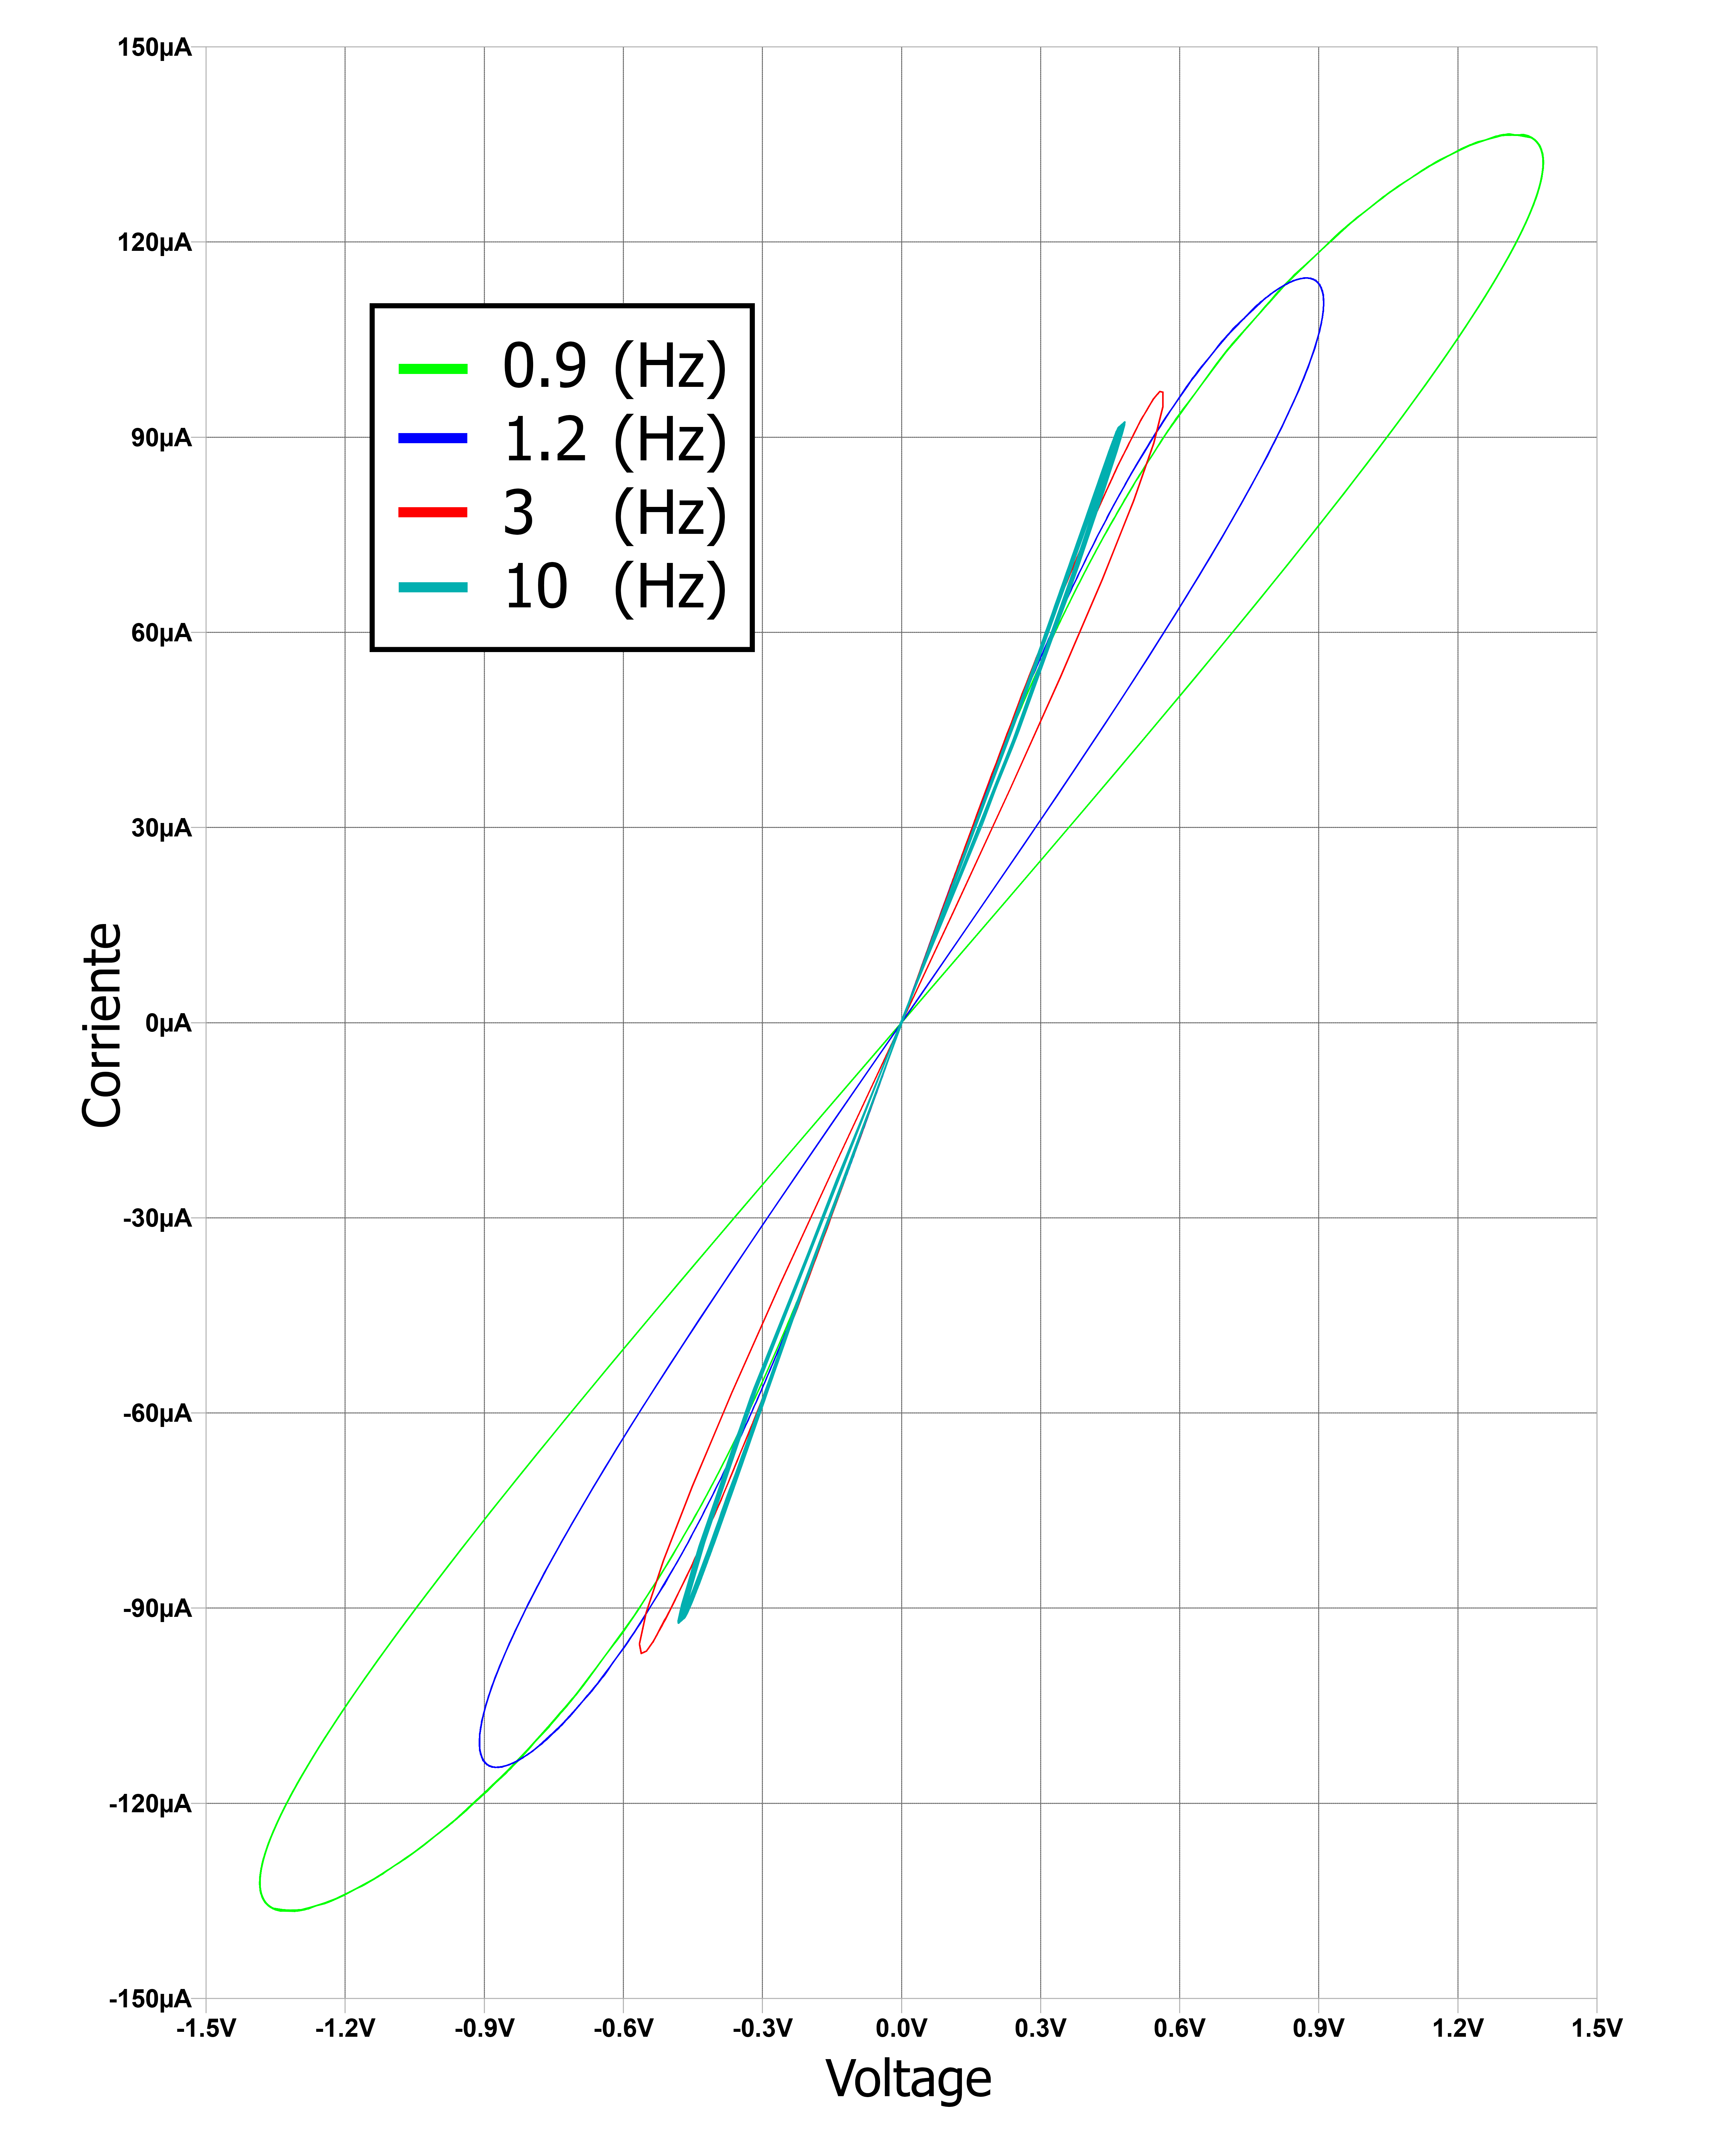
\includegraphics[width=0.85\textwidth]{iv_chua.jpg}
		\caption{Gráfica Tensión-Intensidad del Memristor de Chua ideal para una señal de entrada senoidal con varias frecuencias. Como se puede ver conforme aumenta la frecuencia la gráfica se parece más a la de una resistencia tradicional. Ver \cite{outsiders}}.
		\label{fig:iv_chua}
	\end{figure}\smallskip
	\begin{comment}
		\begin{figure}[h]
		\centering
		\includegraphics[width=0.5\textwidth]{iv_hp.png}
		\caption{Gráfica Tensión-Intensidad del Memristor de HP. Ver \cite{HP}.}
		\label{fig:iv_hp}
	\end{figure}\smallskip
\end{comment}
	\newpage
	
	\section{Variables de estado}
	\label{sec:23}
	\noindent En este trabajo hemos hecho un análisis matemático de la bifurcación del circuito oscilador haciendo uso de técnicas de análisis de reciente estudio, pero primero hay que presentar el circuito y transformar sus ecuaciones eléctricas hasta llegar a una forma matemática con la que poder trabajar. Empecemos analizando el circuito.
	
	\begin{figure}[h]
		\centering
		\includegraphics[width=0.8\textwidth]{circuito.png}
		\caption{Magnitudes del circuito.}
		\label{fig:circuito}
	\end{figure}\smallskip
	
	Aplicanco las leyes de Kirchoff a nuestro circuito, \fref{fig:circuito}, se puede ver que:
	
	\begin{equation}
		i_{LR}\,=\,i_M+i_C,
		\label{eq:kir1}
	\end{equation}
	\begin{equation}
		v_R\,=\,v_L+v_1.
		\label{eq:kir2}
	\end{equation}
	
	Reordenando las anteriores ecuaciones:
	
	\begin{equation}
		i_C\,=\,i_{LR}-i_M,
		\label{eq:kir11}
	\end{equation}
	\begin{equation}
		v_L\,=\,v_R-v_1.
		\label{eq:kir22}
	\end{equation}
	
	Recordando la relación entre la carga y el flujo con la intensidad y la tensión de las ecuaciones \eref{eq:dvdi}, la ecuación del memristor controlado por flujo \eref{eq:fc} y aplicándolo a \eref{eq:kir11} y \eref{eq:kir22} obtenemos:
	
	
	\begin{eqnarray}
		C\,\frac{dv_1}{dt}\,&=&\,i_{LR}-W(\varphi)\,v_1 \label{eq:kir111}, \\ [2mm]
		L\,\frac{di_{LR}}{dt}\,&=&\,R\,i_{LR}-v_1 \label{eq:kir222}, \\ [2mm]
		\frac{d\varphi}{dt}\,&=&\,v_1. \label{eq:kir333}
	\end{eqnarray}\smallskip
	
	Como se pueden ver las variables de estado elegidas son la intensidad en la resistencia y la bobina \bm{$i_{LR}$}, la tensión en el condensador y el memristor \bm{$v_1$} y el flujo en el memristor \bm{$\varphi$}.
	\newpage
	Reordenando las ecuaciones anteriores \eref{eq:kir111}, \eref{eq:kir222} y \eref{eq:kir333} tenemos:
	
	\begin{eqnarray}
		\frac{dv_1}{dt}\,&=&\,\frac{i_{LR}}{C}-W(\varphi)\,\frac{v_1}{C} \label{eq:sis1}, \\ [2mm]
		\frac{di_{LR}}{dt}\,&=&\,\frac{R}{L}\,i_{LR}-\frac{v_1}{L} \label{eq:sis2}, \\ [2mm]
		\frac{d\varphi}{dt}\,&=&\,v_1. \label{eq:sis3}
	\end{eqnarray}\smallskip
	
	Haciendo algunos cambios a las tres anteriores ecuaciones para luego poder trabajar con las ecuaciones obtenemos el siguiente sistema:
    
	\begin{equation}
		\label{eq:sistema1}
		\scalebox{1.2}{$\displaystyle
			\left\{
			\begin{aligned}
				\frac{dx}{dt} &= \alpha (y - W(z)x), \\
				\frac{dy}{dt} &= -\xi x + \beta y, \\
				\frac{dz}{dt} &= x.
			\end{aligned}
			\right.
			$}
	\end{equation}\smallskip
	
	Donde tenemos:
	\begin{equation*}
		x\,=\,v_1, \qquad y\,=\,i_{LR}, \qquad z\,=\,\varphi, \qquad \alpha\,=\,\frac{1}{C}, \qquad \beta\,=\,\frac{R}{L}, \qquad \xi\,=\,\frac{1}{L}.
	\end{equation*}
	
	Escribiendo el sistema \eref{eq:sistema1} de una forma más general:
	
	\begin{equation}
		\label{eq:sistema}
		\scalebox{1.2}{$\displaystyle
			\left\{
			\begin{aligned}
				\frac{dx}{dt} &= a_{11}W(z)x+a_{12}y, \\
				\frac{dy}{dt} &=  a_{21}x+ a_{22}y, \\
				\frac{dz}{dt} &= x.
			\end{aligned}
			\right.
			$}
	\end{equation}\smallskip
	
	Con:
	\begin{equation}
		\label{eq:amatriz}
	\begin{gathered}
		a_{11}=-\alpha=-\frac{1}{C}, \qquad a_{12}=\alpha=\frac{1}{C},\\[2mm]
		a_{21}=-\xi =-\frac{1}{L}, \qquad a_{22}=\beta = \frac{R}{L}.
	\end{gathered}
	\end{equation}\smallskip
	
	Pero del sistema \eref{eq:sistema} aun tenemos que definir $W(z)$. En \cite{chuaoscillator2008} se asume que el comportamiento del memristor se puede aproximar por una ecuacion linear a trozos monótonamente creciente:
	
	\begin{equation}
		q(\varphi)\,=\,b\varphi+0.5(a-b)(|\varphi+1|-|\varphi-1|).
		\label{eq:qf}
	\end{equation}
    \begin{center}
    	$ donde \quad a,b> 0$
    \end{center}
    
    Derivemos la expresión \eref{eq:qf} (recordando la ecuación \eref{eq:myw}) para obtener $W(z)$:

    
    \begin{equation}
    	W(z) = \frac{dq(z)}{dz} =
    	\begin{cases}
    			b,  \quad & z < -1, \\
    			a,  \quad & -1 < z < 1, \\
    			b,  \quad & z > 1.
    	\end{cases}
    	\label{eq:wz}
    \end{equation}
    
    Por último vamos a definir dos matrices auxiliares del sistema \eref{eq:sistema} teniendo en cuenta la función $W(z)$ \eref{eq:wz}
    
    \begin{equation}
    	A_E=\begin{pmatrix*}[c]
    		b \, \cdotp a_{11} & a_{12}\\
    	             a_{21} & a_{22}\\
    	\end{pmatrix*}, \qquad 	A_C=\begin{pmatrix*}
    	a \, \cdotp a_{11} & a_{12}\\
    	a_{21} & a_{22}\\
    	\end{pmatrix*}.
    \end{equation}\smallskip
    
    con sus correspondientes trazas y determinantes:
    \begin{equation}
    \begin{aligned}
    	t_E &= b \cdot a_{11} + a_{22}\\
    	d_E &= b \cdot a_{11}a_{22} - a_{21}a_{12}\\
    	t_C &= a \cdot a_{11} + a_{22}\\
    	d_C &= a \cdot a_{11}a_{22} - a_{21}a_{12}\\
    \end{aligned}
    \end{equation}\smallskip
    
	Ya tenemos las ecuaciones necesarias para empezar el análisis, pero primero veremos en los siguientes capitulos que técnicas estaremos usando para ello.
	\newpage
	\section{Superficies invariantes}
	\label{sec:2.4}
	\noindent A continuación definimos el concepto de superficie invariante para un sistema dinámico tridimensional. Más adelante veremos que el sistema \eref{eq:sistema} posee unas determinadas superficies invariantes. 
	
	\begin{definicion}
		Consideremos, el sistema diferencial:
		
		\begin{equation}
			\label{eq:sergio}
			\frac{dX}{dt}=F(X),\qquad X\in \mathbb{R}^3
		\end{equation}\smallskip
		Se dice que una superficie $S\subset \mathbb{R}^3$ es una superficie invariante para el sistema \eref{eq:sergio} si la solución del sistema diferencial $X(t)$ con condición inicial $X(0)=X_0 \; \in S$ satisface que $X(t) \in S$ para todo $t$ y para todo $X_0 \in S$.
	\end{definicion}\smallskip
	
	A modo de ejemplo, en la \fref{fig:esfera} hemos representado una esfera invariante con varias órbitas de un sistema contenida en ella
	
	\begin{figure}[h]
		\centering
		\includegraphics[width=1\textwidth]{esfera.jpg}
		\caption{Esfera con dos órbitas solución $X_1(t)$, $X_2(t)$ con condiciones iniciales $X_1(0)=X_{0_1}$ y $X_2(0)=X_{0_2}$, contenidas en ella.}
		\label{fig:esfera}
	\end{figure}\smallskip
	\newpage
	
	Desde el Teorema 1 de \cite{ponce}, sabemos que existe un conjunto de superficies invariantes para el sistema \eref{eq:sistema}. La descripción de estas superficies invariantes se detalla en el siguiente resultado. Se enunciará dicho teorema en este trabajo ya que nos será muy importante tenerlo presente.

	\begin{theorem}[Teorema 1 de \cite{ponce}]
		\label{teorema1}
		Consideremos el sistema \eref{eq:sistema} con la función lineal a trozos $q$, dada en \eref{eq:qf}, y la función $W(z)$, dada en \eref{eq:wz}, siendo esta la derivada de dicha función $q$. Para cualquier $h \in \mathbb{R}$, el conjunto:
		
		\begin{equation}
			\label{eq:sh}
			S_h=\left\{(x,y,z)\in \mathbb{R}^3\: : \: H(x,y,z)=h \right\}
		\end{equation}
		donde
		\begin{equation}
			\label{eq:hecuation}
			H(x,y,z)=-a_{22}x+a_{12}y-a_{12}a_{21}z+a_{11}a_{22}q(z).
		\end{equation}\smallskip
		
		\noindent es una superficiente invariante para el sistema \eref{eq:sistema}.
	\end{theorem}
		
		\vspace{0.5cm}\noindent El sistema \eref{eq:sistema} tiene una familia infinita de superficies invariantes en todo $\mathbb{R}^3$, y la dinámica de los mismos es fundamentalmente bidimensional.
	
	\vspace{0.5cm}Como se deduce del Teorema \ref{teorema1} la dinámica del sistema tridimensional \eref{eq:sistema} se puede reducir, aplicando un cambio de variable adecuado, al estudio de un sistema bidimensional.
	
	\vspace{0.5cm}\noindent En este trabajo es necesario incluir la prueba de ello porque los cambios de variable nos permitirán obtener la solución periódica en el circuito.
	
	\newpage
	
	\begin{theorem}[Teorema 2 de \cite{ponce}]
		Consideremos el sistema \eref{eq:sistema}, con la función $W(z)$ dada en \eref{eq:wz}, y supongamos que $a_{22}\neq 0$. La dinámica del sistema \eref{eq:sistema} es equivalente a la dinámica del sistema lineal a trozos bidimensional
		
		\begin{equation}
			\label{eq:sis2ec}
			\left\{
			\begin{gathered}
				\dot{\tilde{x}}=F(\tilde{x})-\tilde{y}, \\[2mm]
				\dot{\tilde{y}}=g(\tilde{x})-h,
			\end{gathered}
			\right.
		\end{equation}
		
		donde
		
		\begin{equation}
			\label{eq:f1}
			F(\tilde{x})=
			\left\{
			\begin{aligned}
				&t_E(\tilde{x}-1)+t_C, \quad &si& \quad \tilde{x}>1,\\
				&t_C\tilde{x}, &si& \quad |\tilde{x}|\leq 1,\\
				&t_E(\tilde{x}+1)-t_C, \quad &si& \quad \tilde{x}<-1,
			\end{aligned}
			\right.
		\end{equation}\smallskip
		
		\begin{equation}
			\label{eq:g1}
			g(\tilde{x})=
			\left\{
			\begin{aligned}
				&d_E(\tilde{x}-1)+d_C, \quad &si& \quad \tilde{x}>1,\\
				&d_C\tilde{x}, &si& \quad |\tilde{x}|\leq 1,\\
				&d_E(\tilde{x}+1)-d_C, \quad &si& \quad \tilde{x}<-1.
			\end{aligned}
			\right.
		\end{equation}\smallskip
		
	\end{theorem}
	
 \vspace{0.5cm} Los subíndices $E$ y $C$ hacen referencia a las zonas $Externas$ y a la zona $Central$ del sistema trizonal \eref{eq:sis2ec}.
	
	\vspace{0.5cm}
		
	\begin{proof}[\textbf{Demostración}]
		 Cuando $a_{22}\neq0$, podemos despejar $x$ de la ecuación $H(x,y,z)=h$, donde $H$ está dada en \eref{eq:hecuation}
		
		\begin{equation}
			\label{eq:xeqn}
			x=\frac{a_{12}}{a_{22}}y+a_{11}q(z)-\frac{a_{12}a_{21}}{a_{22}}z-\frac{h}{a_{22}}.
		\end{equation}\smallskip
		
		\noindent Sutituyendo la expresión de $x$ anterior en la segunda y tercera ecuación de \eref{eq:sistema}, conseguimos
		
		\begin{equation}
			\label{eq:cambyz}
			\left\{
			\begin{aligned}
				&\dot{y}=\alpha_1y-\alpha_2z+a_{11}a_{21}q(z)-\frac{a_{21}h}{a_{22}}, \\[2mm]
				&\dot{z}=\alpha_3y-\alpha_4z+a_{11}q(z)-\frac{h}{a_{22}}.
			\end{aligned}
			\right.
		\end{equation}
		
	    \noindent con
		
		\begin{equation}
			\label{eq:alphamatriz}
			\begin{aligned}
				&\alpha_1=\frac{a_{22}^2+a_{12}a_{21}}{a_{22}}, \qquad &\alpha_2=\frac{a_{21}^2a_{12}}{a_{22}},\\[2mm]
				&\alpha_3=\frac{a_{12}}{a_{22}}, \qquad &\alpha_4=\frac{a_{12}a_{21}}{a_{22}}.
			\end{aligned}
		\end{equation}\smallskip
		
		\noindent Seguidamente, considerando el siguiente cambio de variable
		
		\begin{equation}
			\label{eq:xytilde}
			\begin{aligned}
				&\tilde{x}=z, \\[2mm]
				&\tilde{y}=\alpha_1z-\alpha_3y+\frac{h}{a_{22}}
			\end{aligned}
		\end{equation}\smallskip
		
		 \noindent el sistema \eref{eq:cambyz} se puede escribir en la forma \eref{eq:sis2ec}, con lo que finaliza la demostración del resultado.
		
	\end{proof}
	
	\vspace{0.5cm}Una breve explicación del significado de los anteriores teoremas. Supongamos que $a_{22}\neq 0$ y tomamos una condición inicial $X_0=(x_0,y_0,z_0)$. Esto nos fija la superficie invariante $S_{h_0}$ donde está la órbita del sistema con condición inicial $X_0$. Obviamente el valor de $h_0$ es $h_0=H(x_0,y_0,z_0)$, con $H$ dada en \eref{eq:hecuation}.
	
	\vspace{0.5cm}A partir del valor $h=h_0$, determinamos la solución $\left( \tilde{x}(t),\tilde{y}(t) \right)$ del sistema \eref{eq:sis2ec} con condición inicial $\tilde{x}(0)=z_0$, $\; \tilde{y}(0)=\alpha_1z_0-\alpha_3y_0+\frac{h_0}{a_{22}}$. La solución $(x(t),y(t),z(t))$ del sistema \eref{eq:sistema} con condición inicial $(x_0,y_0,z_0)$ está dada por:
	
	\begin{equation}
		\label{eq:solsis}
		\scalebox{1.1}{$\displaystyle
			\left\{
			\begin{aligned}
				z(t)&=\tilde{x} \\[3mm]
				y(t)&= \frac{\alpha_1\tilde{x}(t)+\frac{h_0}{a_{22}}-\tilde{y}(t)}{\alpha_3}\\[3mm]
				x(t)&=\frac{a_{12}}{a_{22}}\left( \frac{\alpha_1\tilde{x}(t)+\frac{h_0}{a_{22}}-\tilde{y}(t)}{\alpha_3} \right) +a_{11}q(\tilde{x}(t))-\frac{a_{12}a_{21}}{a_{22}}\tilde{x}(t)-\frac{h_0}{a_{22}}
			\end{aligned}
			\right.
			$}
	\end{equation}\smallskip
	
	\begin{comment}
	\vspace{0.5cm}Una breve explicación del significado de los anteriores teoremas. Supongamos que $a_{22}\neq 0$, si elegimos una condición inicial de nuestro sistema que se encuentre dentro de alguna superficie de las que hemos definido en \eref{eq:sh}, entonces la solución del sistema siempre estará contenida en dicha superficie. Es decir, mirando las ecuaciones \eref{eq:xytilde}; con $\tilde{x}$ calculamos la $z$, con $\tilde{y}$ podemos despejar y calcular la $y$ (recordemos que $h$ ya la hemos definido con las condiciones iniciales), y finalmente con la ecuación \eref{eq:xeqn} calculamos la $x$ .Hemos reducido un sistema tridimensional a uno bidimensional y conocemos el plano a trozos $h$ donde estará contenia la solución del sistema.
	\end{comment}
	
	\begin{comment}
	\vspace{0.5cm}La función $W(z)$ puede ser discontinua, esto dependerá de las carácterísticas del memristor. Aún así esta posible discontinuidad no nos afectará en nuestro trabajo como se demuestra en la sección 3 de \cite{ponce} donde los autores demuestran como pasar en cualquier caso de un modelo discontinuo a un modelo reducido continuo. Además en el artículo de Chua de 2008, ver \cite{chuaoscillator2008} donde se presenta el circuito que estamos estudiando en este trabajo, los autores presentan una aproximación de lo que podrían ser la gráfica flujo-carga del memristor caracterizada por la ecuación \eref{eq:qfz} y la suponen continua.
	\end{comment}
	
	\vspace{0.5cm}Nuestro nuevo sistema de dimensión dos tiene tres zonas como vemos en \eref{eq:sis2ec}, sin embargo en este trabajo nos centraremos en dos de ellas, puesto que buscaremos oscilaciones periódicas bizonales. Se hace esta aclaración ya que parte del trabajo que haremos más adelante nos permitiría hacer el estudio de tres zonas, pero no es el objetivo de este trabajo.

	
	\chapter{Sistemas Dinámicos Continuos}
	En este capítulo haremos un repaso de sistemas dinámicos continuos lineales a trozos puesto que como hemos visto en el sistema \eref{eq:sistema} hemos reducido nuestro circuito a un sistema de este tipo. Lo que necesitamos ahora es encontrar la o las soluciones de nuestro sistema y estudiar su estabiliad, la base que necesitamos para ello lo veremos en este capítulo.
	\newpage
	\section{Sistemas lineales planos}
	\label{sec:sislinplanos}
	En esta sección vamos a analizar los sistemas dinámicos continuos de 2 ecuaciones lineales de primer orden con coeficientes constantes, ya que posteriormente describiremos nuestro circuito de esta forma.
	Antes que nada hay que definir lo que es un sistema dinámico continuo:
	
	\begin{definicion}
		Un sistema dinámico es un conjunto de ecuaciones de cambio que describen la evolución temporal de algún fenómeno, que puede ser de cualquier naturaleza (eléctrico, económico, cinegético...), de manera que el estado presente del sistema viene determinado por los estados anteriores. El estado del sistema queda descrito por sus variables de estado. Cuando la evolución se estudia considerando el tiempo como una variable 
		continua, decimos que el sistema es continuo y para analizar este tipo de sistemas la regla determinista que lo gobierna es su sistema de ecuaciones diferenciales.
	\end{definicion}
	
	Un sistema de este tipo tiene la siguiente forma:
	
	\begin{equation}
		\label{eq:edo2}
		\scalebox{1.2}{$\displaystyle
			\left\{
			\begin{aligned}
				\dot{x}\,=\,\frac{dx}{dt}\,=\,a_{11}x(t)+a_{12}y(t)+b_1 \\
				\dot{y}\,=\,\frac{dy}{dt}\,=\,a_{21}x(t)+a_{22}y(t)+b_2
			\end{aligned}
			\right.
			$}
	\end{equation}\smallskip
	
	Escribiendo el sistema \eref{eq:edo2} en forma matricial:
	
	\begin{equation}
		\label{eq:matrxedo2}
		\scalebox{1.2}{$\displaystyle
		\begin{pmatrix}
			\dot{x}\\
			\dot{y}\\
		\end{pmatrix} =
		\begin{pmatrix}
			a_{11} & a_{12}\\
		    a_{21} & a_{22}\\
		\end{pmatrix} 
		\begin{pmatrix}
			x\\
			y\\
		\end{pmatrix} + 
		\begin{pmatrix}
			b_1\\
			b_2\\
		\end{pmatrix}
		$}
	\end{equation} \smallskip
	
	Ecribiendo el sistema \eref{eq:matrxedo2} de forma mas simplificada:
	
	\begin{equation}
		\label{eq:sisautonomo}
		\dot{X}\,=\,AX+B
	\end{equation}\smallskip
	
	Cuando $B=\vec{0}$ el sistema se dice homogéneo. Por el contrario cuando $B\neq\vec{0}$ el sistema se dice no homogéneo. Esto es importante saberlo pues los métodos para solucionar estos tipos de sistemas no son las mismos.
	
	Tambien hay que tener en cuenta las condiciones iniciales del sistema:
	
	\begin{equation}
		\label{eq:ci}
		\scalebox{1.2}{$\displaystyle
			\left\{
			\begin{aligned}
				x(0)=x_0 \\
			    y(0)=y_0
			\end{aligned}
			\right.
			$}
	\end{equation}\smallskip
	
	Escribiendo el sistema \eref{eq:ci} en forma matricial:
	
	\begin{equation}
		\label{cimat}
		X(t_0)=\begin{pmatrix}
			x(0)\\y(0)
		\end{pmatrix}=\begin{pmatrix}
		x_0\\y_0
		\end{pmatrix}=X_0
	\end{equation}\smallskip
	
	Al conjunto del sistema y a sus condiciones iniciales se les denomina \\ \textbf{\textit{Problema de Valor Inicial (PVI)}}: 
	
	\begin{equation}
	\label{eq:pvi}
	\scalebox{1.2}{$\displaystyle
		\left\{
		\begin{aligned}
			&\dot{X}=AX+B &\rightarrow& \textit{Sistema Diferencial (S.D.)}\\
			&X(t_0)=X_0 &\rightarrow& \textit{Condiciones Iniciales (C.I.)}
		\end{aligned}
		\right.
		$}
    \end{equation}\smallskip
	
	Lo primero y más importante que se debe hacer con este tipo de problemas es comprobar la existencia y unicidad de sus soluciones.
	\newpage
	\begin{theorem}\label{thm:interesante}
		Existencia y unicidad \\[2mm]
		\textit{Sean $A$ y $B$ continuas en un intervalo $I\subseteq  \mathbb{R}$, que continene el punto $X(t_0)$ entonces el P.V.I. tiene una única solución definida en dicho intervalo $I$ para cualquier vector $X_0 \in \mathbb{R}^2$}. Además, si el P.V.I. tiene coeficientes constantes en $A$ y $B$ la solución está definida en $\mathbb{R}$.
	\end{theorem}
	\vspace{4mm}
	
	Las soluciones del sistema son el conjunto de puntos \eref{eq:puntos} para cada instante de tiempo que forman una curva en el plano de fases $xy$.
	\begin{equation}
		\label{eq:puntos}
		X(t)=\begin{pmatrix}
			x(t) \\ y(t)
		\end{pmatrix}
	\end{equation}\smallskip
	
	Ahora lo lógico sería hablar de como resolver este tipo de problemas ya que es nuetsro objetivo, pero no lo vamos a hacer ya que nosotros no usaremos el método tradicional de autovalores y autovectores para ello, vamos a utilizar otra técnica de reciente estudio con la que no hará falta esto, la veremos mas adelante.\\[0.5cm]
	Por último veamos como obtener y analizar los puntos de equilibrio del Sistema Lienal Plano. Primero escribamos el sistema \eref{eq:edo2} de otra forma para ver los siguientes apartados mejor:
	\begin{equation}
		\label{eq:sv}
		\scalebox{1.2}{$\displaystyle
			\left\{
			\begin{aligned}
				\dot{x}\,=\,\frac{dx}{dt}\,=S(x,y) \\
				\dot{y}\,=\,\frac{dy}{dt}\,=V(x,y)
			\end{aligned}
			\right.
			$}
	\end{equation}\smallskip
	
	\begin{definicion}
		Los puntos $(\overline{x},\overline{y})$ que anulan simultaneamente las funciones $S$ y $V$ del sistema \eref{eq:matrxedo2} se denominan Puntos de Equilibrio o Críticos del sistema:
	\end{definicion}

	\begin{eqnarray}
		\label{eq:crit}
			\begin{pmatrix}
				0\\
				0\\
			\end{pmatrix} =
			&\begin{pmatrix}
				a_{11} & a_{12}\\
				a_{21} & a_{22}\\
			\end{pmatrix}&
			\begin{pmatrix}
				\overline{x}\\
				\overline{y}\\
			\end{pmatrix} + 
			\begin{pmatrix}
				b_1\\
				b_2\\
			\end{pmatrix}\nonumber \\[4mm]
			&\begin{pmatrix}
			a_{11} & a_{12}\\
			a_{21} & a_{22}\\
			\end{pmatrix}&
			\begin{pmatrix}
			\overline{x}\\
			\overline{y}\\
			\end{pmatrix} = 
			\begin{pmatrix}
			-b_1\\
			-b_2\\
			\end{pmatrix} \nonumber \\[4mm]
			&A\,\overline{X}=-b
	\end{eqnarray}\smallskip
	
	Si el $det(A)\neq0$ \eref{eq:crit} el sistema posee un único punto de equilibrio, este punto se dice solucion constante del sistema.
    \\[0.5cm]
    Veamos esto más en profundiad, primero tenemos que saber que el sistema que tenemos \eref{eq:sv} se denomina \textit{\textbf{Autónomo}} ya que la variable independiente $\bm{t}$ no aparece de manera explícita en los segundos términos.
    \newpage
    Ahora lo que haremos es una translación del punto de equilibrio para que esté en el origen $\begin{pmatrix} 0 \\ 0
    \end{pmatrix}$ en caso de no estarlo:
    
	\begin{equation}
		\label{eq:trans}
		\scalebox{1.2}{$\displaystyle
			\left\{
			\begin{aligned}
				\tilde{X}=x-\overline{x} \\
				\tilde{Y}=y-\overline{y}
			\end{aligned}
			\right.
			$}
	\end{equation}\smallskip
	
	Por lo que ahora tenemos:
	
	\begin{equation}
		\label{eq:trans2}
		\scalebox{1.2}{$\displaystyle
			\left\{
			\begin{aligned}
				\frac{d\tilde{X}}{dt}\,=S(\tilde{X}-\overline{x},\tilde{Y}-\overline{x}) \\
				\frac{d\tilde{Y}}{dt}\,=V(\tilde{X}-\overline{x},\tilde{Y}-\overline{x})
			\end{aligned}
			\right.
			$}
	\end{equation}\smallskip
	Donde el punto $\begin{pmatrix} 0 \\ 0 \end{pmatrix}$ es el punto de equilibrio. \\[0.5cm]
	Lo que verermos a continuacion es la disposicion de las soluciones al rededor del punto de equilibrio y la estabilidiad o no del mismo. Considerando el sistema autónomo lineal con punto de equilibrio en el origen que hemos obtenido tras el cambio de variable:
	
	\begin{eqnarray}
		\label{eq:trans3}
			\begin{pmatrix}
				\dot{x}\\
				\dot{y}\\
			\end{pmatrix} =
			&\underbrace{\begin{pmatrix}
				a_{11} & a_{12}\\
				a_{21} & a_{22}\\
			\end{pmatrix}}&
			\begin{pmatrix}
				x\\
				y\\
			\end{pmatrix} \nonumber \\[1mm]
			&A&
	\end{eqnarray} \smallskip
	
	Como vemos con el cambio de variable no se ha modificado la matriz $A$ que es la que nos dirá todo respecto a la estabilidad del punto crítico, veremos los tres casos que se estudian en este trabajo: Foco Asintóticamente Estable, Foco Asintóticamente Inestable y Centro. Pero hay muchos mas y, por supuesto, combinaciones de todos ellos, lo cual complica estos problemas en gran medida.\\[0.5cm]
	Para saber la estabilidad de los puntos debemos estudiar el polinomio caracteristico de la matriz $A$:
	
	\begin{equation}
		\label{eq:equilibrio}
		A=\begin{pmatrix}
			a_{11} & a_{12}\\
			a_{21} & a_{22}\\
		\end{pmatrix}\rightarrow\left\{
		\begin{aligned}
		\det(A )&= a_{11}a_{22}-a_{12}a_{21} \\
		\tr(A) &= a_{11}+a_{22}
	    \end{aligned}
		\right.
	\end{equation}\smallskip
	
	\begin{eqnarray}
		\begin{aligned}
		P_A(\lambda)=&\lambda^2-\tr(A)\lambda+\det(A) \nonumber \\[1mm]
		&\lambda^2-\tr(A)\lambda+\det(A)=0 \nonumber \\[1mm]
		\textit{Autovalores}\rightarrow \quad &\lambda=\frac{\tr(A)\pm \sqrt{\tr(A)^2-4\,\det(A)}}{2}
	    \end{aligned}
	\end{eqnarray}
	
	\newpage

	{\Large\textbullet\quad Foco Asintóticamente Estable}\\[0.5cm]
	
	Las curvas solucion tienden al punto crítico. Este caso se da para: 
	\begin{itemize}
		\item \textbf{$\tr$}$\bm{(A)<0}$
		\item \textbf{$\tr$}$\bm{(A)^2-4\, \det(A)<0}$
	\end{itemize}
	
	\begin{figure}[h]
		\centering
		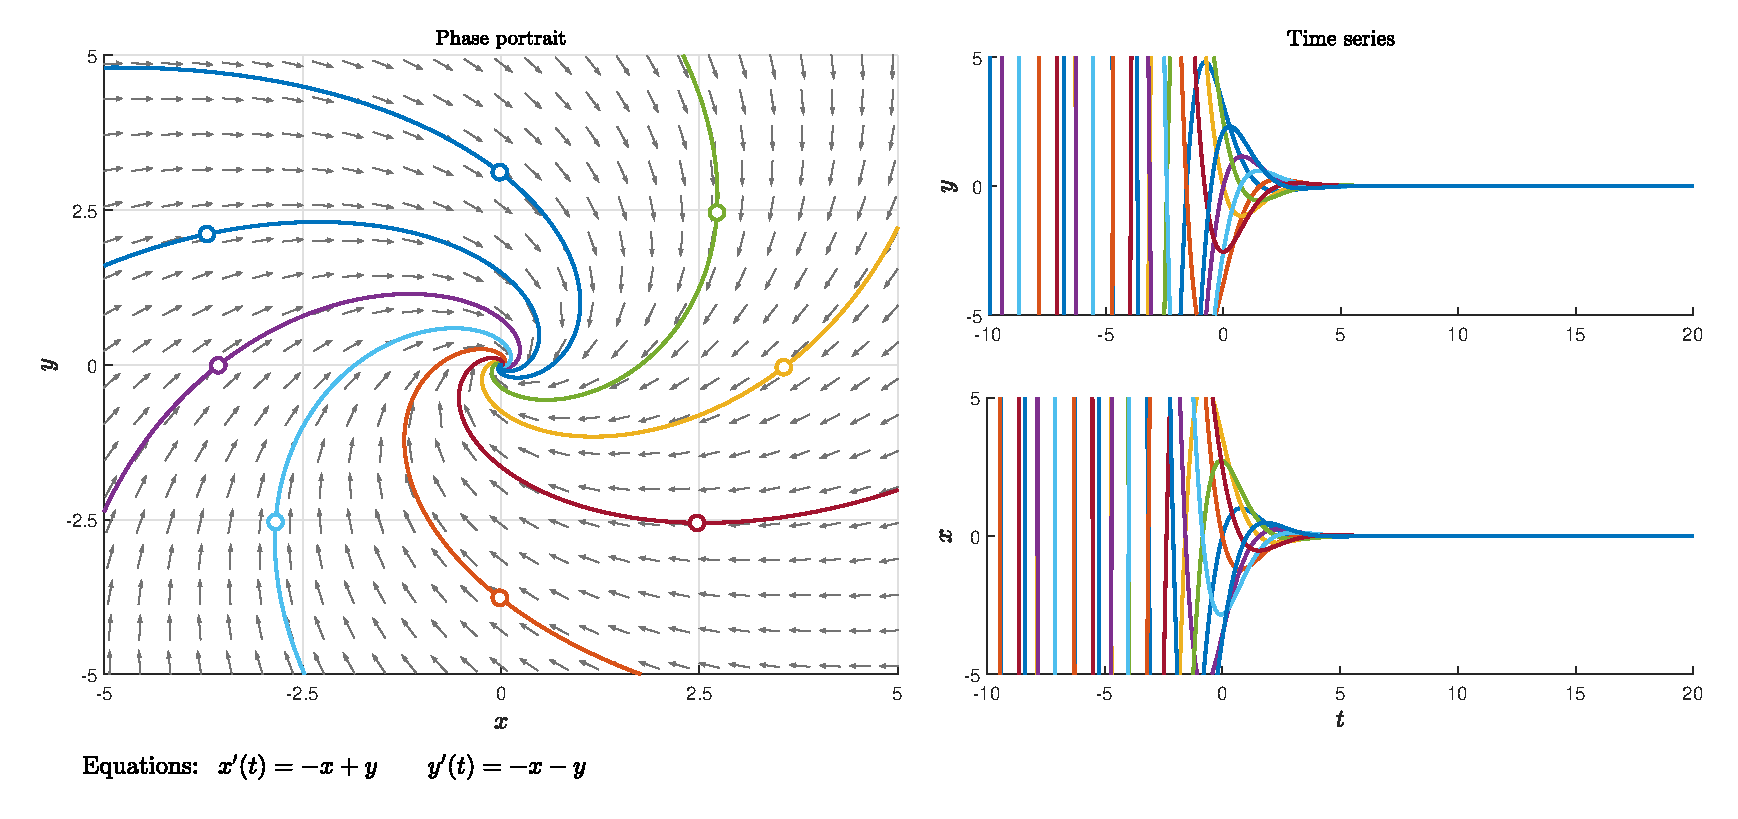
\includegraphics[width=1\textwidth]{estable.eps}
		\caption{Foco Asintóticamente Estable visto en el plano de fases $xy$ (izquierda) y la variacion de $x$ e $y$ en el tiempo (derecha).}
		\label{fig:estable}
	\end{figure}\smallskip
	
	La matriz $A$ del la \fref{fig:estable} es 
	$\begin{pmatrix*}[r]
		-1 & 1 \\
		-1 & -1
	\end{pmatrix*}$
	
	\begin{align*}
		&\bullet\quad \tr(A)=-2<0 \\[2mm]
		&\bullet\quad \tr(A)^2-4\, \det(A)=4-4(2)<0
	\end{align*}
	
	\newpage
	
	{\Large\textbullet\quad Foco Asintóticamente Inestable}\\[0.5cm]
	
	Las curvas solucion tienden al alejarse del punto crítico. Este caso se da para: 
	\begin{itemize}
		\item \textbf{$\tr$}$\bm{(A)>0}$
		\item \textbf{$\tr$}$\bm{(A)^2-4\, \det(A)<0}$
	\end{itemize}
	
	\begin{figure}[h]
		\centering
		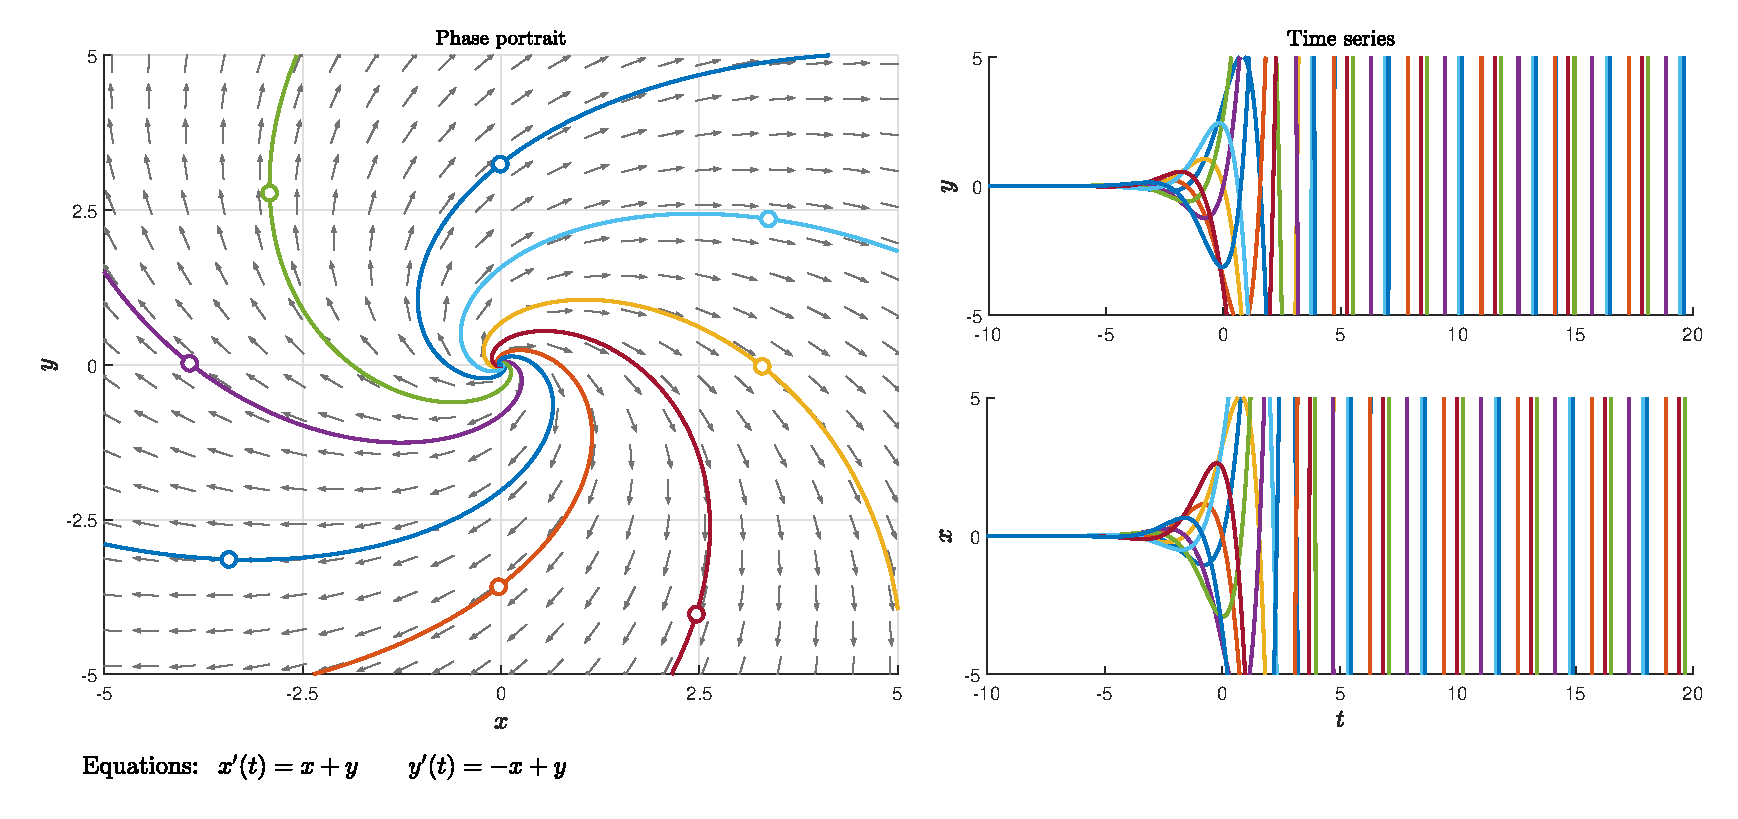
\includegraphics[width=1\textwidth]{inestable.eps}
		\caption{Foco Asintóticamente Inestable visto en el plano de fases $xy$ (izquierda) y la variacion de $x$ e $y$ en el tiempo (derecha).}
		\label{fig:inestable}
	\end{figure}\smallskip
	
	La matriz $A$ del la \fref{fig:inestable} es 
	 $\begin{pmatrix*}[r]
		 1 & 1 \\
		-1 & 1
	 \end{pmatrix*}$
	
	\begin{align*}
		&\bullet\quad \tr(A)=2>0 \\[2mm]
		&\bullet\quad \tr(A)^2-4\, \det(A)=4-4(2)<0
	\end{align*}
	
	\newpage
	
    {\Large\textbullet\quad Centro}\\[0.5cm]
    
    Las curvas solucion son concéntricas al punto crítico. Este caso se da para: 
    \begin{itemize}
    	\item \textbf{$\tr$}$\bm{(A)=0}$
    	\item \textbf{$\tr$}$\bm{(A)^2-4\, \det(A)<0}$
    \end{itemize}
    
    \begin{figure}[h]
    	\centering
    	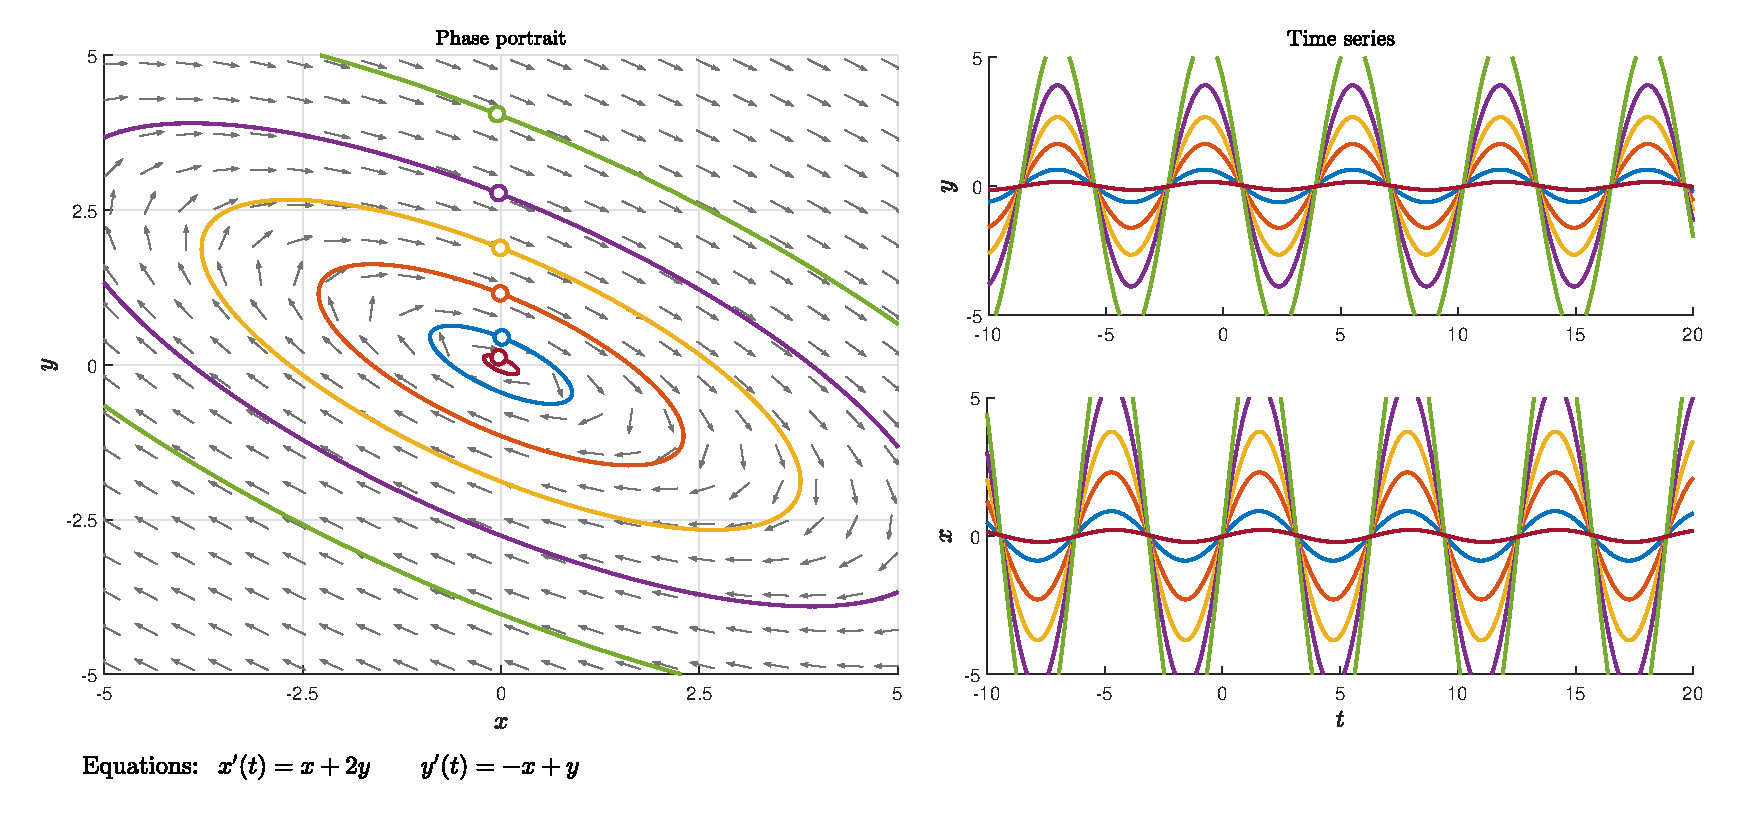
\includegraphics[width=1\textwidth]{centro.eps}
    	\caption{Centro en el plano de fases $xy$ (izquierda) y la variacion de $x$ e $y$ en el tiempo (derecha).}
    	\label{fig:centro}
    \end{figure}\smallskip
    
    La matriz $A$ del la \fref{fig:centro} es 
    $\begin{pmatrix*}[r]
    	1 & 2 \\
    	-1 & -1
    \end{pmatrix*}$
    
    \begin{align*}
    	&\bullet\quad \tr(A)=1-1=0 \\[2mm]
    	&\bullet\quad \tr(A)^2-4\, \det(A)=0-4(1)<0
    \end{align*}
	
	\newpage
	\section{Sistemas lineales a trozos bizonales}
	\label{sistrobiz}
	En esta sección vamos a ver como estudiar los sistemas continuos dinámicos lineales a trozos de dos zonas y veremos sus propiedades de cara a la obtención de una órbita periódica y estudiar su amplitud y periodo.\\[0.5cm] También veremos como utilizar las formas canónicas para reducir el número de parámetros que influyen en el sistema y como apoyarnos en dichas formas canónicas y las propiedades que nos portan a la hora de estudiar la oscilacion periódica de nuestro circuito.
	
	\begin{definicion}
		Un sistema dinámico continuo lineal a trozos plano con dos zonas es un sistema de ecuaciones diferenciales con la siguiente forma:
	\end{definicion}
	
	\begin{equation}
		\frac{dx}{dt}=\dot{x}=S(x)=
		\label{eq:biz1}
		\scalebox{1}{$\displaystyle
			\left\{
			\begin{aligned}
			 A_1x+b_1\quad si \quad x^T\cdotp w+\delta \leq 0 \\
			 A_2x+b_2\quad si \quad x^T\cdotp w+\delta < 0
			\end{aligned}
			\right.
			$}
	\end{equation}\smallskip
	Donde $x=(x_1,x_2)^T\in \mathbb{R}^2$, las matrices $A_1$ y $A_2$ son reales de orden $2$, además\\ $b_1$, $b_2$, $w$ $\in \mathbb{R}^2$ con $w\neq\vec{0}$ y $\delta \in \mathbb{R}$ y se satisface la condición de continuidad
	
	\begin{equation}
		A_1x+b_1=A_2x+b_2 
	\end{equation}\smallskip
	
	Sobre la recta de separación de las dos zonas:\quad $x^T\cdotp w+\delta = 0$ \\[0.5cm]
	
	\textbf{\textcolor{red}{EXISTENCIA Y UNICICDAD DE SISTEMA 3.14}}

	Para cada $x^0 \in \mathbb{R}^2$, el problema de valores iniciales \eref{eq:pvi2} tiene una solución única $x(t)$ definida para todo $t$ real.
	
	\begin{equation}
		\label{eq:pvi2}
		\scalebox{1.2}{$\displaystyle
			\left\{
			\begin{aligned}
				&\dot{x}=S(x)\\
				&x(0)=x^0
			\end{aligned}
			\right.
			$}
	\end{equation}\smallskip
	
	 A continuación veremos la forma canónica mas común para los sistemas bizonales que coloca la recta separación en el eje de ordenadas $x_1=0$.
	
	\begin{definicion}
		Todo sistema dinámico continuo lineal a trozos plano con dos zonas puede escribirse de la siguiente forma:
	
	\begin{equation}
		\dot{x}=S(x)=
		\label{eq:lien}
		\scalebox{1}{$\displaystyle
			\left\{
			\begin{aligned}
				B_1x+c\quad si \quad x_1 \leq 0 \\
				B_2x+c\quad si \quad x_1 < 0
			\end{aligned}
			\right.
			$}
	\end{equation}\smallskip
	\textbf{\textcolor{red}{$S(x)$? pero yo tengo dos variables x1 y x2, es $S(x_1,x_2)$? }}
	
	Con $x=(x_1,x_2)^T, c\in \mathbb{R}^2$ y las matrices $B_1$, $B_2$ comparten sus dos últimas columnas por continuidad, esto es:
	\begin{equation}
		B_1-B_2 = \left(B_1-B_2\right)e_1e_1^T 
	\end{equation}\smallskip
	
	\textbf{\textcolor{red}{multiplicado los e?}}
	
	Siendo $e_1=(1,0)^T$ el primer vector de la base canónica $\mathbb{R}^2$. Además, por continuidad también, se puede ver que $c_1=c_2=c$.
    \end{definicion}\smallskip

	
	\textbf{Demostración}: Basta con realizar una simetría para que el vector $w$ normal a la recta $x^T\cdotp w+\delta=0$, se transforme en el vector $e_1=(1,0)^T$ se puede hacer usando matrices de Householder \cite{docvic}. Por último con una translación hacemos que la nueva recta de separación $x_1=0$ (ahora vertical) pase por el origen. Por lo que el sistema queda con la forma:
	\textbf{\textcolor{red}{y que pasa con $\delta$? por que la recta se llama $x_1$, la puedo llamar solo x? menos lio con $\dot{x}_1$. Pero $x^T$ y $w$ son vectores? en lugar de la recta x=0 se podria usar la x=-1?}}
	
	\begin{equation}
		\dot{x}=
		\label{eq:lien2}
		\scalebox{1}{$\displaystyle
			\left\{
			\begin{aligned}
			B_1x+c_1\quad si \quad x_1 \leq 0 \\
			B_2x+c_2\quad si \quad x_1 < 0
			\end{aligned}
			\right.
			$}
	\end{equation}\smallskip
	
	Con $B_1$ y $B_2$ matrices de orden 2 y $c_1, c_2 \in \mathbb{R}^2$. Nuevamente por continuidad se debe satisfacer:
	
	\begin{equation}
		\label{eq:b1b2}
		B_1x+c_1=B_2x+c_2 \qquad si \quad x_1=0
	\end{equation}\smallskip
	
	Como el punto $(0,0)^T$ está en la recta de separación $x_1=0$, sustituyendo en \eref{eq:b1b2} se tiene que $c_1=c_2$ por lo que:
	
	\begin{equation}
		B_1x=B_2x \qquad si \quad x_1=0
	\end{equation}\smallskip
	
	Como el vector $(0,1)^T$ está sobre la recta de separación $x_1=0$, se tiene por tanto que las dos últimas columnas de $B_1$ y $B_2$ son iguales, y además no olvidemos que  antes hemos visto que $c_1=c_2=c$.
	\\ [0.5cm]
	Se ha reducido bastante el número de parámetros, ahora tenemos 8, 6 de ellos vienen de las matrices $B_1$ y $B_2$ y 2 de $c$. Para seguir reduciendo parámetros tengamos en cuenta que estamos buscando oscilaciones y que no aparecerán en sistemas unidimensionales por lo que el primer término de las segundas columnas de las matrices $B_1$ y $B_2$ no puede ser nulo (condición de observabilidad \cite{onsimplyfing}). Mediante el cambio de variable oportuno lo convertiremos en $(-1)$ aquí lo vemos, en primer lugar escribimos el sistema \eref{eq:lien2} de la siguiente manera:
	
	\begin{equation}
		\begin{pmatrix*}[r]
			\dot{x}_1 \\ \dot{x}_2
		\end{pmatrix*}=
		\label{eq:lie-1}
		\scalebox{1.2}{$\displaystyle
			\left\{
			\begin{aligned}
				\begin{pmatrix*}[r]
					b_{11}^1 & b_{12} \\
					b_{21}^1 & b_{22}
				\end{pmatrix*}\begin{pmatrix*}[r]
				x_1\\x_2
				\end{pmatrix*}+\begin{pmatrix*}[r]
				c_1 \\ c_2
				\end{pmatrix*} \quad si \quad x_1 \leq 0 \\
				\begin{pmatrix*}[r]
					b_{11}^2 & b_{12} \\
					b_{21}^2 & b_{22}
				\end{pmatrix*}\begin{pmatrix*}[r]
				x_1\\x_2
				\end{pmatrix*}+\begin{pmatrix*}[r]
					c_1 \\ c_2
				\end{pmatrix*} \quad si \quad x_1 < 0
			\end{aligned}
			\right.
			$}
	\end{equation}\smallskip
	
	Y le aplicamos el cambio de variable (recordando que $b_{12}\neq0$): 
	
	\begin{equation}
		\label{eq:cambio}
		X_2=-b_{12}\,x_2-c_1\quad \rightarrow \quad x_2=\frac{-X_2-c_1}{b_{12}}
	\end{equation}\smallskip

	Para el caso $x_1\leq 0$ del sistema \eref{eq:lie-1} aplicando el cambio de variable \eref{eq:cambio}:
	
	\begin{equation}
		\label{eq:q1}
	\begin{aligned}
		\dot{x}_1&=b_{11}^1x_1+b_{12}x_2+c-1=b_{11}^1x_1+b_{12}\left(\frac{-X_2-c_1}{b_{12}}\right)+c_1=b_{11}^1x_1-X_2 \\[2mm]
		\dot{X}_2&=-b_{12}\dot{x}_2=-b_{12}\left(b_{21}^1x_1+b_{22}x_2+c_2\right) \\[2mm]
		&=-b_{12}b_{21}^1x_1+b_{22}\left(-b_{12}x_2\right)-b_{12}c_2  \\[2mm]
		&=-b_{12}b_{21}^1x_1+b_{22}\left(X_2+c_1\right)-b_{12}c_2 \\[2mm]
		&=-b_{12}b_{21}^1x_1+b_{22}X_2+b_{22}c_1-b_{12}c_2
	\end{aligned}
	\end{equation}\smallskip
	
	
	De forma análoga para $x_1>0$ del sistema \eref{eq:lie-1}:
	\begin{equation}
		\label{eq:q2}
		\scalebox{1.2}{$\displaystyle
			\left\{
			\begin{aligned}
			&\dot{x}_1=b_{11}^2x_1-X_2 \\[2mm]
			&\dot{X}_2=-b_{12}b_{21}^2x_1+b_{22}X_2+b_{22}c_1-b_{12}c_2
		\end{aligned}
		\right.
		$}
	\end{equation}\smallskip
	
	Sustituyendo \eref{eq:q1} y \eref{eq:q2} en el sistema \eref{eq:lie-1}, tomando $c_{11}^i=b_{11}^i \: ; \: \\c_{21}^i=-b_{12}b_{21}^i \: ; \: c_{22}=b_{22} \: ; \: d_2=b_{22}c_1-b_{12}c_2$ y renombrando $X_2$ como $x_2$:
	
	\begin{equation}
		\begin{pmatrix*}[r]
			\dot{x}_1 \\ \dot{x}_2
		\end{pmatrix*}=
		\label{eq:lie-12}
		\scalebox{1.2}{$\displaystyle
			\left\{
			\begin{aligned}
				\begin{pmatrix*}[r]
					c_{11}^1 & -1 \\
					c_{21}^1 & c_{22}
				\end{pmatrix*}\begin{pmatrix*}[r]
				x_1\\x_2
				\end{pmatrix*}+\begin{pmatrix*}[c]
				0 \\ d_2
				\end{pmatrix*} \quad si \quad x_1 \leq 0 \\
				\begin{pmatrix*}[r]
					c_{11}^2 & -1 \\
					c_{21}^2 & c_{22}
				\end{pmatrix*}\begin{pmatrix*}[r]
				x_1\\x_2
				\end{pmatrix*}+\begin{pmatrix*}[c]
				0 \\ d_2
				\end{pmatrix*} \quad si \quad x_1 < 0
			\end{aligned}
			\right.
			$} 
	\end{equation}\smallskip
	
	Hemos conseguido eliminar otros dos parámetros del sistema, además solo hemos realizado cambios lineales por lo que las matrices características son semejantes, es decir, no hemos variado las características del sistema. Lo que nos queda es ya pasar a la famosa forma canónica de Liénard:
	
	
	\begin{theorem}\label{t2}
		Existe un cambio de variable que transforma el sistema \eref{eq:lie-12} en la forma canónica de Liénard, sin modificar la traza y el determinanate de la matriz característica del sistema ya que son invariates algebraicos:
	\end{theorem}
	
	\begin{equation}
		\begin{pmatrix*}[r]
			\dot{x}_1 \\ \dot{x}_2
		\end{pmatrix*}=
		\label{eq:lienard}
		\scalebox{1.2}{$\displaystyle
			\left\{
			\begin{aligned}
				\begin{pmatrix*}[r]
					t & -1\\
					d & 0
				\end{pmatrix*}\begin{pmatrix*}[r]
				x_1\\x_2
				\end{pmatrix*}-\begin{pmatrix}
				0\\a
				\end{pmatrix} \quad si \quad x_1\leq 0 \\
				\begin{pmatrix*}[r]
					T & -1\\
					D & 0
				\end{pmatrix*}\begin{pmatrix*}[r]
				x_1\\x_2
				\end{pmatrix*}-\begin{pmatrix}
					0\\a
				\end{pmatrix} \quad si \quad x_1 > 0
			\end{aligned}
			\right. \qquad con\quad a \in \left\{-1,0,1\right\}
			$}
	\end{equation}\smallskip

	
	\textbf{Demostración}: Usando el siguiente cambio de variable:
	
	\begin{equation}
		\label{eq:cambioo}
		X_2=c_{22}x_1+x_2\quad \rightarrow \quad x_2=X_2-c_{22}x_1
	\end{equation}\smallskip
	
	Para el caso $x_1\leq 0$ del sistema \eref{eq:lie-12} aplicando el cambio de variable \eref{eq:cambioo}:
	
		\begin{equation}
		\label{eq:cambio2}
		\begin{aligned}
			\dot{x}_1&=c_{11}^1x_1-x_2=c_{11}^1x_1-(X_2-c_{22}x_1)=x_1(c_{11}^1+c_{22})-X_2 \\[2mm]
			\dot{X}_2&=c_{22}\dot{x}_1+\dot{x}_2=c_{22}(c_{11}^1x_1-x_2)+(c_{21}^1x_1+c_{22}x_2+d_2) \\[2mm]
			&=c_{22}c_{11}^1x_1-c_{22}x_2+c_{21}^1x_1+c_{22}x_2+d_2 \\[2mm]
			&=x_1(c_{22}c_{11}^1+c_{21})+d_2
		\end{aligned}
		\end{equation}\smallskip
	
	De forma análoga para $x_1>0$ del sistema \eref{eq:lie-12}:
	\begin{equation}
		\label{eq:cambio22}
		\scalebox{1.2}{$\displaystyle
			\left\{
			\begin{aligned}
				&\dot{x}_1=x_1(c_{11}^2+c_{22})-X_2 \\[2mm]
				&\dot{X}_2=x_1(c_{22}c_{11}^2+c_{21}^2)+d_2
			\end{aligned}
			\right.
			$}
	\end{equation}\smallskip
	
	Sustituyendo \eref{eq:cambio2} y \eref{eq:cambio22} en el sistema \eref{eq:lie-12}, tomando $t=c_{11}^1+c_{22} \: ; \:\\ d=c_{22}c_{11}^1+c_{21}^1 \: ; \:  T=c_{11}^2+c_{22} \: ; \: D=c_{22}c_{11}^2+c_{21}^2$ y renombrando $X_2$ como $x_2$:
	
	\begin{equation}
		\begin{pmatrix*}[r]
			\dot{x}_1 \\ \dot{x}_2
		\end{pmatrix*}=
		\label{eq:lienard2}
		\scalebox{1.2}{$\displaystyle
			\left\{
			\begin{aligned}
				\begin{pmatrix*}[r]
					t & -1\\
					d & 0
				\end{pmatrix*}\begin{pmatrix*}[r]
				x_1 \\ x_2
				\end{pmatrix*}+\begin{pmatrix}
					0\\d_2
				\end{pmatrix} \quad si \quad x_1\leq 0 \\
				\begin{pmatrix*}[r]
					T & -1\\
					D & 0
				\end{pmatrix*}\begin{pmatrix*}[r]
				x_1 \\ x_2
				\end{pmatrix*}+\begin{pmatrix}
					0\\d_2
				\end{pmatrix} \quad si \quad x_1 > 0
			\end{aligned}
			\right. 
			$}
	\end{equation}\smallskip

	Siendo $t,d,T,D$ las respectivas trazas $(t,T)$ y determinantes $(d,D)$ de las matrices caracteristicas de cada uno de los sitemas a la derecha y a la izquierda de la recta de separación $x_1=0$, que como ya hemos visto, no hemos modificado sus propiedades pues todos los cambios aplicados han sido lineales.\\[0.5cm]

	Por último vamos a ajustar $d_2$. Si $d_2=0$ entonces el sistema ya sería igual que \eref{eq:lienard} pero con el parámetro $a=0$. Si $d_2\neq0$ hay que aplicar el siguiente cambio:
	
	\begin{equation}
		\label{eq:cambiod2}
		X_1=\frac{x_1}{|d_2|} \qquad X_2=\frac{x_2}{|d_2|}
	\end{equation}\smallskip
	
	Por lo que $X_1$ tiene el mismo sigo que $x_1$ y la recta de separación sería $X_1=0$.\\[0.5cm]
	Para el caso $X_1\leq 0$ del sistema \eref{eq:lienard2} aplicando el cambio de variable \eref{eq:cambiod2}:
	
	\begin{equation}
		\label{eq:q3}
		\begin{aligned}
			&\dot{X}_1=\frac{\dot{x}_1}{|d_2|}=\frac{tx_1-x_2}{|d_2|}=t\frac{x_1}{|d_2|}-\frac{x_2}{|d_2|}=tX_1-X_2\\[2mm]
			&\dot{X}_2=\frac{\dot{x}_2}{|d_2|}=\frac{dx_1-0+d_2}{|d_2|}=d\frac{x_1}{|d_2|}+\frac{d_2}{|d_2|}=dX_1+\frac{d_2}{|d_2|}\\[2mm]
		\end{aligned}
	\end{equation}\smallskip
	
	De forma análoga para $x_1>0$ del sistema \eref{eq:lie-12}:
	\begin{equation}
		\label{eq:q4}
		\scalebox{1}{$\displaystyle
			\left\{
			\begin{aligned}
				&\dot{X}_1=TX_1-X_2 \\[2mm]
				&\dot{X}_2=DX_1+\frac{d_2}{|d_2|}
			\end{aligned}
			\right.
			$}
	\end{equation}\smallskip
	
	Démonos cuenta que cuando dividimos $d_2$ entre su valor absoluto lo que estamos obteniendo es $-1,1,0$ dependiendo de si $d_2$ es negativo, positivo o cero, por lo que usaremos la funcion signo \textit{sgn}:
	
	\begin{equation}
		\label{eq:sgn}
		sgn(d_2)=\left\{
		\begin{aligned}
		1 \qquad si  \quad d_2>0 \\
		0 \qquad si  \quad d_2=0 \\
		-1 \qquad si \quad d_2<0 
    	\end{aligned}
		\right.
	\end{equation}\smallskip
	
	Sustituyendo \eref{eq:q3} y \eref{eq:q4} en el sistema \eref{eq:lienard2}, tomando $a=-sgn(d_2)$ \textcolor{red}{a=-d2 eso esta bien??} y renombrando $X_1$ como $x_1$ y $X_2$ como $x_2$:
	
	
	\begin{equation}
		\begin{pmatrix*}[r]
			\dot{x}_1 \\ \dot{x}_2
		\end{pmatrix*}=
		\label{eq:lienardfinal}
		\scalebox{1.2}{$\displaystyle
			\left\{
			\begin{aligned}
				\begin{pmatrix*}[r]
					t & -1\\
					d & 0
				\end{pmatrix*}\begin{pmatrix*}[r]
					x_1 \\ x_2
				\end{pmatrix*}-\begin{pmatrix}
					0\\a
				\end{pmatrix} \quad si \quad x_1\leq 0 \\
				\begin{pmatrix*}[r]
					T & -1\\
					D & 0
				\end{pmatrix*}\begin{pmatrix*}[r]
					x_1 \\ x_2
				\end{pmatrix*}-\begin{pmatrix}
					0\\a
				\end{pmatrix} \quad si \quad x_1 > 0
			\end{aligned}
			\right. 
			$}
	\end{equation}\smallskip
	
	Para ubicar de una manera más gráfica lo que tenemos en \eref{eq:lienardfinal}:
	\begin{equation}
		\label{eq:lienardfinalgr}
		\begin{gathered}
			\begin{pmatrix*}[r]
				\dot{x}_1\\ \dot{x}_2
			\end{pmatrix*}= \begin{pmatrix*}[r]
				t & -1 \\ d & 0
			\end{pmatrix*} \begin{pmatrix*}[r]
				x_1 \\ x_2
			\end{pmatrix*}-\begin{pmatrix*}[c]
				0 \\ a
			\end{pmatrix*} \qquad 
			\rule[-40pt]{1.5pt}{80pt} \qquad 
			\begin{pmatrix*}[r]
				\dot{x}_1\\ \dot{x}_2
			\end{pmatrix*}= \begin{pmatrix*}[r]
				T & -1 \\ D & 0
			\end{pmatrix*} \begin{pmatrix*}[r]
				x_1 \\ x_2
			\end{pmatrix*}-\begin{pmatrix*}[c]
				0 \\ a
			\end{pmatrix*} \\ x_1=\;0
		\end{gathered}
	\end{equation}\smallskip
	\newpage
	Podemos darnos cuenta de que las ecuaciones corresponden a las dos zonas izquierda y derecha de la recta de separación $x_1=0$ así que vamos a hacer unos cambios de nombres a las variables del sistema \eref{eq:lienardfinal} simplemente para que los nombres sean un poco mas descriptivos. Finalmente el sistema en la forma canónica de Liènard nos queda de la siguiente manera:
	
	\begin{equation}
		\begin{pmatrix*}[r]
			\dot{x} \\ \dot{y}
		\end{pmatrix*}=
		\label{eq:lienardrl}
		\scalebox{1.2}{$\displaystyle
			\left\{
			\begin{aligned}
				\begin{pmatrix*}[r]
					T_L & -1\\
					D_L & 0
				\end{pmatrix*}\begin{pmatrix*}[r]
					x \\ y
				\end{pmatrix*}-\begin{pmatrix}
					0\\a
				\end{pmatrix} \quad si \quad x\leq 0 \\
				\begin{pmatrix*}[r]
					T_R & -1\\
					D_R & 0
				\end{pmatrix*}\begin{pmatrix*}[r]
					x \\ y
				\end{pmatrix*}-\begin{pmatrix}
					0\\a
				\end{pmatrix} \quad si \quad x > 0
			\end{aligned}
			\right. 
			$}
	\end{equation}\smallskip
	
	De una manera más gráfica sería:
	
	\begin{equation}
		\label{eq:lienardrlgr}
		\begin{gathered}
			\begin{pmatrix*}[r]
				\dot{x}\\ \dot{y}
			\end{pmatrix*}= \begin{pmatrix*}[r]
				T_L & -1 \\ D_L & 0
			\end{pmatrix*} \begin{pmatrix*}[r]
				x \\ y
			\end{pmatrix*}-\begin{pmatrix*}[c]
				0 \\ a
			\end{pmatrix*} \qquad 
			\rule[-40pt]{1.5pt}{80pt} \qquad 
			\begin{pmatrix*}[r]
				\dot{x}\\ \dot{y}
			\end{pmatrix*}= \begin{pmatrix*}[r]
				T_R & -1 \\ D_R & 0
			\end{pmatrix*} \begin{pmatrix*}[r]
				x \\ y
			\end{pmatrix*}-\begin{pmatrix*}[c]
				0 \\ a
			\end{pmatrix*} \\ x=\;0
		\end{gathered}
	\end{equation}\smallskip
	
	\newpage
	
	\chapter{Semiaplicaciones de Poincaré}
	\label{sec:4}
	En el estudio de sistemas dinámicos, la \textbf{aplicación de Poincaré} es una herramienta de gran utilidad para estudiar el conportamiento de un determinado sistema. Se trata de delimitar una superficie o recta (llamada sección de Poincaré), en el espacio de fases de nuestro sistema, de tal manera que las curvas solución de nuestro sistema transpasen dicha sección para poder estudiar así el comportamiento de las trayectorias. Lo interesante de esta aplicación es que lo que estudiamos son los puntos de intersección con la sección de Poincaré, aunque no podemos obviar el comportamiento de la trayectoria y el tiempo para el estudio.\\[0.5cm]
	
	\begin{figure}[h]
		\centering
		\includegraphics[width=0.8\textwidth]{aplipoincare2.jpg}
		\caption{Punto $y_0$ y su imagen $\tilde{y_0}$ mediante la aplicación de Poincaré. Esta órbita no es periódica}
		\label{fig:aplipoincare2}
	\end{figure}\smallskip
	\textcolor{red}{parrafo entero}
\noindent Como vemos en la \fref{fig:aplipoincare2} la dinámica de estudio sería establecer un punto inicial $y_0$, definir una sección de Poincaré que corte a la curva solución y por último analizar como avanza dicha curva en el tiempo esperando a que corte de nuevo a la sección de Poincaré. Finalmente si la órbita vuelve a cortar en el mismo punto $y_0=\tilde{y_0}$ diremos que dicha órbita es periódica.
	\newpage
	
	En este trabajo hablaremos de la \textit{\textbf{semiaplicación de Poincarè}}, es decir, analizaremos una de las dos mitades de la orbita. Esto lo haremos ya que como nuestro estudio es de un sistema a trozos \eref{eq:lienardrl}, ya tenemos una separación en la recta $x=0$ la cual usaremos de sección de Poincaré, y como a la izquierda y a la derecha de dicha sección tenemos sistemas diferentes debemos estudiarlos de manera independiente.
	
	\begin{figure}[h]
		\centering
		\includegraphics[width=0.9\textwidth]{poincaLR.jpg}
		\caption{Semiaplicación derecha e izquierda las cuales forman una órbita periódica}
		\label{fig:poincaLR}
	\end{figure}\smallskip
	
	\textcolor{red}{cambiar parrafo}
	Tendremos un punto de corte $y_0$ de nuestra órbita solución en la sección de Poincarè y buscaremos el siguiente punto de corte $y_1$ mediante la semiaplicación izquierda, finalmente mediante la semiaplicación derecha comprobamos si la órbita vuelve a cortar a la sección de Poincarè en el mismo punto $y_0$ (órbita periódica, ver \fref{fig:poincaLR}) o si no corta en el mismo punto $y_0$ (órbita no periódica).
	
	\vspace{0.5cm}Para definir de forma apropiada una semiaplicación de Poincarè, consideraremos el sistema \eref{eq:edo2}, que mediante los cambios de variable adeacuados podemos escribir en forma canónica de Lienard como ya hemos visto a lo largo de la Sección \ref{sistrobiz}. En dicha sección se hace para un sistema a trozos, pero para esta parte consideraremos un único sistema, que puede ser el derecho o el izquierdo, por lo que la nomenclatura que usaremos en esta sección para dicho sistema será:
	
		\begin{equation}
		\label{eq:lienardsolo}
		\begin{pmatrix*}[r]
			\dot{x}\\ \dot{y}
		\end{pmatrix*}= \begin{pmatrix*}[r]
			T & -1 \\ D & 0
		\end{pmatrix*} \begin{pmatrix*}[r]
			x \\ y
		\end{pmatrix*}-\begin{pmatrix*}[c]
			0 \\ a
		\end{pmatrix*}
	\end{equation}\smallskip
	\newpage
	
	Definiendo la sección de Poincaré como $\varSigma=\left\{(x,y)^T\in \mathbb{R}^2:x=0\right\}$ donde nos referiremos con $\varSigma^L$ a la zona izquierda de la sección y $\varSigma^R$ a la zona derecha de la sección (recordemos que los índices $R$ y $L$ harán alusión a las zonas derecha e izquierda). Si evaluamos la primera ecuación de \eref{eq:lienardsolo} en la sección de Poincarè $\varSigma$, tenemos $\dot{x}|_{\varSigma}=-y$, pudiéndose deducir el sentido de la órbita:
	
	\begin{itemize}
		\item La órbita va de $\varSigma^L$ a $\varSigma^R$ para $y<0$.
		\item La órbita va de $\varSigma^R$ a $\varSigma^L$ para $y>0$.
	\end{itemize}
	
	Asumiremos $a^2+D^2\neq0$, ya que de no ser así, curva solución no cortaría de nuevo a $\varSigma$. Esto se puede deducir estudiando la segunda ecuación del sistema \eref{eq:lienardsolo} para el caso contrario $a=D=0 \longrightarrow \dot{y}=Dx+a=0$, y por lo tanto $\dot{y}$ es constante.
	
	\vspace{0.5cm}Vamos a centrarnos en la zona izquierda de la sección de Poicaré $\varSigma^L$, la cual se define de la siguiente manera:

	\vspace{0.5cm}
	\begin{definicion}
		\label{def6}
		Consideremos el punto $(0,y_0)\in \varSigma$ con $y_0\geq0$, denotaremos por $\phi(t)=(\phi_1(t),\phi_2(t))$ la solución del sistema \eref{eq:lienardsolo}, que para el instante inicial $t=0$ cumple que $\phi(0)=(0,y_0)$. Si existe un valor de tiempo $\tau>0$ para el que se cumple $\phi_1(\tau)=0$ y $\phi_1(t)<0$ para todo $t\in(0,\tau)$, decimos que la imagen de $y_0$ mediante la semiaplicación izquierda de Poincaré $P_L(y_0)=\phi_2(\tau)\leq0$. El valor de tiempo $\tau$ se denomina semitiempo de vuelo izquierdo.
	\end{definicion}
	
	\vspace{0.5cm}La definción de la semiaplicación de Poincaré derecha $P_R$ puede hacerse a partir de la semiaplicación izquierda ya que el sistema \eref{eq:lienardsolo} no varia sus propiedades cuando se le aplica el cambio de variable $(x,y,a)\longleftrightarrow(-x,-y,-a)$.
	
	\newpage
	
	\vspace{0.5cm} A continuación se puede ver la representación gráfica de la semiaplicación izquierda, \fref{fig:semiL}, y derecha, \fref{fig:semiR}, con la nomenclatura adoptada y las correspondientes definiciones de sus dominios $\mathcal{D}$. En \cite{caracterizacion} se puede consultar más en profundidad la definición de estos.

	
	\begin{figure}[h]
		\centering
		\includegraphics[width=0.6\textwidth]{semiL.jpg}
		\caption{Semiaplicación de Poincaré Izquierda}
		\label{fig:semiL}
	\end{figure}\smallskip
	
	\vspace{0.5cm}Dominio de definición de la semiaplicación izquierda:
	
	\vspace{0.5cm}
	
	\begin{equation}
		\label{eq:dl}
		\scalebox{1.3}{$\displaystyle
		\begin{aligned}
		P_L:\mathcal{D}_L\subset [\,0,+\infty) &\longrightarrow ( -\infty,0\, ]\\[2mm]
		y_0 &\longrightarrow y_1
	\end{aligned}
	$}
	\end{equation}
	
	\newpage
	
	\begin{figure}[h]
		\centering
		\includegraphics[width=0.6\textwidth]{semiR.jpg}
		\caption{Semiaplicación de Poincaré Derecha}
		\label{fig:semiR}
	\end{figure}\smallskip
	
	\vspace{0.5cm}Dominio de definición de la semiaplicación derecha:
	
	\vspace{0.5cm}
	
	\begin{equation}
		\label{eq:dr}
		\scalebox{1.3}{$\displaystyle
			\begin{aligned}
				P_R:\mathcal{D}_R\subset (-\infty,0\,] &\longrightarrow [\,0, +\infty)\\[2mm]
				y_1 &\longrightarrow y_2
			\end{aligned}
			$}
	\end{equation}
	
	\vspace{0.5cm} La Definición \ref{def6} invita a estudiar la dinámica del sistema mediante el cálculo explícito de sus soluciones, este es el método clásico, el cual conlleva una gran cantidad de posibles casos debidos a los espectros (conjunto de autovalores) de las matrices de cada sistema. Casos que deben analizarse uno a uno, aplicando diferentes herramientas para cada uno de ellos. Esto se traduce en gran dificultad para el estudio y obtención de aparentemente distintos resultados para el mismo sistema dependiendo de qué herramienta matemática usemos para su análisis. Para evitar esta problemática usaremos la caracterización integral de la semiaplicación de Poincaré, la cual presentaremos en la sección \ref{sec41}, y puede verse en \cite{caracterizacion}.
	\newpage
	
	\section{Caracterización integral de la semiaplicación de Poincare}
	\label{sec41}
	
	\vspace{0.5cm} Antes de ver las expresiones de la Caracterización Integral se va a presentar el \textit{\textbf{Valor Principal de Cauchy}} ya que se utiliza en las mismas.
	\begin{definicion}
	
	 Consideremos un intervalo $[a,b]$ que contiene al origen y una funcion $f$ continua en $[a,b] \setminus \left\{0\right\}$, el Valor Principal de Cauchy se define como:
	
	\begin{equation}
		\scalebox{1.2}{$\displaystyle
			PV\left\{\int_{a}^{b}f(x)dx\right\}= \lim_{\epsilon \to 0^+}\left(
			\int_{a}^{-\epsilon}f(x)dx \; + \; 
			\int_{+\epsilon}^{b}f(x)dx
			\right)
			$}
	\end{equation}\smallskip
	
    \end{definicion}
    
	\noindent En \cite{caracterizacion},\cite{pv} se puede consultar más en profundidad el Valor Principal de Cauchy.
	
	\vspace{1cm} En la siguiente página presentaremos las expresiones de la caracterizacion integral izquierda y derecha y algunas propiedades de las mismas.
	
	\newpage
	
	\vspace{0.5cm}\noindent \textbf{Caracterización integral de la semiaplicación de Poincaré izquierda:}
	\begin{equation}
		\label{eq:caracl}
		\scalebox{1.2}{$\displaystyle
			PV\left\{\int_{y_1}^{y_0}\frac{-y}{D_Ly^2-aT_Ly+a^2}dy\right\}=\frac{k_L\pi T_L}{D_L\sqrt{4D_L-T_L^2}}
			$}
	\end{equation}\smallskip
	
	\noindent donde
	
	\begin{equation*}
		k_L=
		\label{eq:kl}
		\scalebox{1.2}{$\displaystyle
			\left\{
			\begin{aligned}
				0 \qquad si \quad a>0 \\
				1 \qquad si \quad a=0 \\
				2 \qquad si \quad a<0 
			\end{aligned}
			\right. 
			$}
	\end{equation*}\smallskip
	
	\vspace{0.5cm}
	
	\begin{equation*}
		\scalebox{1.2}{$\displaystyle
		y_0 \in \mathcal{D}_L \quad e \quad y_1\in P_L(\mathcal{D}_L)
		$}
	\end{equation*}\smallskip
	
	\noindent Siendo $ P_L(\mathcal{D}_L)$ el recorrido de $P_L$.
	
	
	\vspace{2cm}\noindent \textbf{Caracterización integral de la semiaplicación de Poincaré derecha:}
	\begin{equation}
		\label{eq:caracr}
		\scalebox{1.2}{$\displaystyle
			PV\left\{\int_{y_1}^{y_0}\frac{-y}{D_Ry^2-aT_Ry+a^2}dy\right\}=\frac{-k_R\pi T_R}{D_R\sqrt{4D_R-T_R^2}}
			$}
	\end{equation}\smallskip
	
	\noindent donde
	
	\begin{equation*}
		k_R=
		\label{eq:kr}
		\scalebox{1.2}{$\displaystyle
			\left\{
			\begin{aligned}
				0 \qquad si \quad a<0 \\
				1 \qquad si \quad a=0 \\
				2 \qquad si \quad a>0 
			\end{aligned}
			\right. 
			$}
	\end{equation*}\smallskip
	
	\begin{equation*}
		\scalebox{1.2}{$\displaystyle
			y_1 \in \mathcal{D}_L \quad e \quad y_1\in P_L(\mathcal{D}_L)
			$}
	\end{equation*}\smallskip
	
	\noindent Siendo $ P_R(\mathcal{D}_R)$ el recorrido de $P_R$.
	
	\vspace{1cm} En las siguientes figuras veremos ejemplos de $P_L$, $P_R$ y $P_R^{-1}$ que forman una órbita periódica (\fref{fig:aplipoincareLRcerrado}, \fref{fig:aplipoincareL-Rcerrado}) o por el contrario no formando dicha órbita periódica (\fref{fig:aplipoincareLR}, \fref{fig:aplipoincareL-R}).
	
	\newpage
	
	 \begin{figure}[h]
		\centering
		\includegraphics[width=1\textwidth]{aplipoincareLR.jpg}
		\caption{Semiaplicación izquierda del punto $y_0$ y semiaplicación derecha del punto $y_1$ con diferentes valores $y_0$,$y_2$ por lo que no se ha cerrado la órbita.}
		\label{fig:aplipoincareLR}
	\end{figure}\smallskip
	
	\newpage
	
	\begin{figure}[h]
		\centering
		\includegraphics[width=1\textwidth]{aplipoincareL-R.jpg}
		\caption{Semiaplicación izquierda del punto $y_0$ y semiaplicación inversa derecha del punto $y_0$ con diferentes valores $y_1$,$y_2$ por lo que no se ha cerrado la órbita.}
		\label{fig:aplipoincareL-R}
	\end{figure}\smallskip
	
	\newpage
	
	\begin{figure}[h]
		\centering
 		\includegraphics[width=1\textwidth]{aplipoincareLRcerrado.jpg}
		\caption{Semiaplicación izquierda del punto $y_0$ y semiaplicación derecha del punto $y_1$ con mismos valores $y_0$,$y_2$ por lo que si se ha cerrado la órbita, formándose una órbita periódica.}
		\label{fig:aplipoincareLRcerrado}
	\end{figure}\smallskip
	
	\newpage
	
	\begin{figure}[h]
		\centering
		\includegraphics[width=1\textwidth]{aplipoincareL-Rcerrado.jpg}
		\caption{Semiaplicación izquierda del punto $y_0$ y semiaplicación inversa derecha del punto $y_0$ con mismos valores $y_1$,$y_2$ por lo que si se ha cerrado la órbita formándose una órbita periódica.}
		\label{fig:aplipoincareL-Rcerrado}
	\end{figure}\smallskip
	
	\newpage
	
	\vspace{0.5cm}\noindent Para encontrar una oscilación periódica debemos buscar valores $y_0^*\in \mathcal{D}_L$, $y_1^*\in \mathcal{D}_R$ tales que
	
	\begin{equation*}
		\label{eq:ej1}
		\scalebox{1.2}{$\displaystyle
			\left\{
			\begin{aligned}
				P_L(y_0^*)=y_1^*, \\
				P_R(y_1^*)=y_0^* ,
			\end{aligned}
			\right. 
			$}
	\end{equation*}\smallskip
	
	\noindent de manera equivalente
	
	\begin{equation*}
		\label{eq:ej2}
		\scalebox{1.2}{$\displaystyle
			\left\{
			\begin{aligned}
				P_L(y_0^*)=y_1^*, \\
				P_R^{-1}(y_0^*)=y_1^*,
			\end{aligned}
			\right. 
			$}
	\end{equation*}\smallskip
	
	\noindent de modo que
	
	\begin{equation*}
		\scalebox{1.2}{$\displaystyle
		P_L(y_0^*)=P_R^{-1}(y_0^*),
		$}
	\end{equation*}
	
	\begin{equation*}
		\scalebox{1.2}{$\displaystyle
		y_0^* \in \mathcal{D}_L \cap P_R(\mathcal{D}_R),
		$}
	\end{equation*}
	
	\begin{equation*}
		\scalebox{1.2}{$\displaystyle
			y_1=P_L(y_0) \quad con \quad y_0\in\mathcal{D}_L, \qquad y_1=P_R^{-1}(y_0) \quad con \quad y_0\in P_R\left(\mathcal{D}_R\right).
			$}
	\end{equation*}
	
	\vspace{0.5cm}\noindent Recordando de los intervalos de dominio \eref{eq:dl}-\eref{eq:dr} que $y_0\geq0$ e $y_1\leq0$, si representamos las curvas de nivel $y_1=P_L(y_0)$ e $y_1=P_R^{-1}(y_0)$ y observamos el cuarto cuadrante veríamos una gráfica como la de la \fref{fig:graficaejemplo}.
	
		\begin{figure}[h]
		\centering
		\includegraphics[width=0.8\textwidth]{graficaejemplo.jpg}
		\caption{Punto de corte entre $y_1=P_L(y_0)$ e $y_1=P_R^{-1}(y_0)$}
		\label{fig:graficaejemplo}
	\end{figure}\smallskip
	
	\newpage
	
	\vspace{0.5cm} Vamos a ver un ejemplo de la Caracterización Integral de la semiaplicación de Poincaré en MATLAB para entender un poco mejor la estrategia de busqueda de la oscilación periódica.
	
	\vspace{1cm}\lstinputlisting[style=Matlab-editor]{Ejemplo_1.m}
	
	\vspace{1cm}\lstinputlisting[style=Matlab-bw]{cwejem1.m}
	
	\vspace{1cm}\noindent Función usada en ``Ejemplo 1'':
	\vspace{0.5cm}\lstinputlisting[style=Matlab-editor]{semipoinca.m}
	
	\newpage
	
	La función \textit{semipoinca} es la aplicación directa de la caracterización integral en MATLAB. Veamos que se se está haciendo:
	
	\vspace{0.5cm}\noindent Primero vamos a reordenar por ejemplo la expresión de la caracterización izquierda \eref{eq:caracl} (con la expresión de la caracterización derecha el procedimiento es el mismo):
	
	\begin{equation}
			\label{eq:eje1}
		\scalebox{1.2}{$\displaystyle
		\begin{gathered}
			\int_{y_1}^{y_0}\frac{-y}{D_Ly^2-aT_Ly+a^2}dy-\frac{k_L\pi T_L}{D_L\sqrt{4D_L-T_L^2}}=0
		\end{gathered}
			$}
	\end{equation}\smallskip
	
	\noindent como vemos en \textit{semipoinca} tenemos como argumentos de entrada $k,a,T,D,y_0$ y como argumento de salida $y_1$, por lo que la ecuación \eref{eq:eje1} se puede reducir a:
	
		\begin{equation}
		\label{eq:eje3}
		\scalebox{1.2}{$\displaystyle
				f(y_1)=0
			$}
	\end{equation}\smallskip
	
	\noindent finalmente la ecuación \eref{eq:eje3} ya está en la forma adecuada para resolverla con la función \textit{fzero} de MATLAB, introduciendo como punto inicial $-y_0$. La función \textit{fzero} resuelve de manera numérica una ecuación tipo $f(x)=0$ a partir de un punto inicial $x_0$ dado.
	
	\vspace{0.5cm}\noindent El código de ``Ejemplo 1'' describe las características de los sistemas a la izquierda y a la derecha, establece un punto de prueba $y_0=1.5$ y llama a la función \textit{semipoinca} para calcular la semiaplicación izquierda y la semiaplicación inversa derecha. Como se ve obtenemos valores diferentes, de hecho la semiaplicación izquierda tiene un valor mayor que la derecha, gráficamente podría ser perfectamente lo representado en la \fref{fig:aplipoincareL-R}.
	\newpage
	
	Como hemos visto para usar \textit{fzero} necesitamos un punto inicial, sin entrar mucho en detalle de resolución numérica, este punto cuanto más cercano a la solución lo eligamos mas fiable y rápida será dicha solución, por ello vamos a representar de manera gráfica las semiaplicaciones izquierda y derecha para un intervalo de puntos $y_0 \in [0\;\;10]$ y veamos si existe un punto de corte que nos indique que para un $y_0$ las imágenes izquierda y derecha son las mismas.
	
	\vspace{1cm}\lstinputlisting[style=Matlab-editor]{Ejemplo_2.m}
	
	\vspace{1cm}En este caso usamos \textit{fplot} la cual va evaluando la función continuamente con valores de $y_0$ desde cero hasta diez, se pintará de rojo la semiaplicación izquierda y de azul la semiaplicación derecha 
	\newpage
	
	\begin{figure}[h]
		\centering
		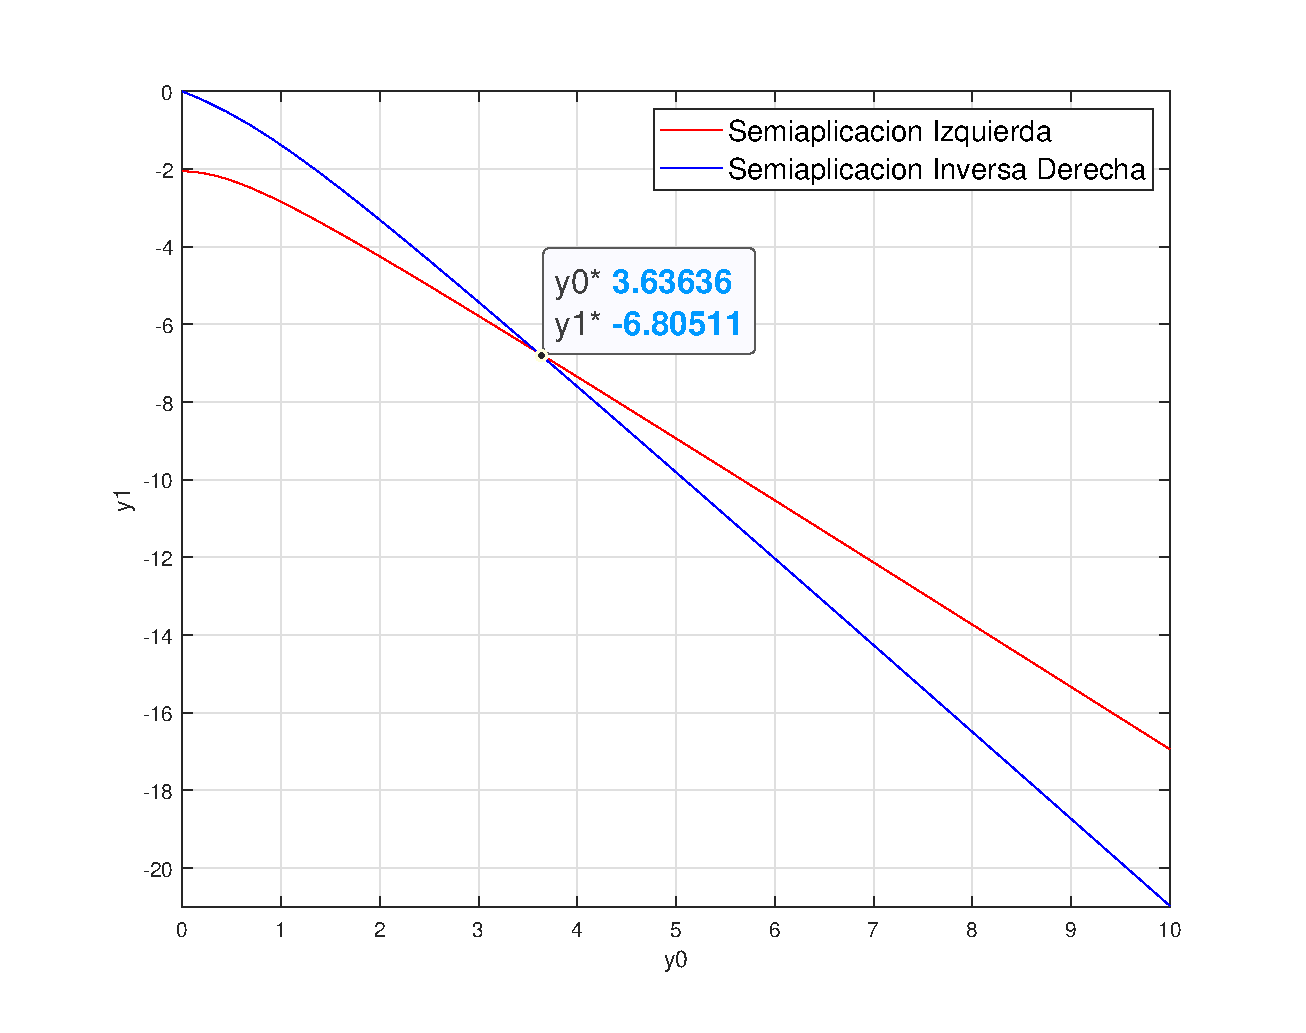
\includegraphics[width=1\textwidth]{g1ejem2.eps}
		\caption{Gráfica obtenida de la semiapliación izquierda y la semiaplicación inversa derecha en el cuarto cuadrante de ``Ejemplo 2''}
		\label{fig:ejem2_2}
	\end{figure}\smallskip
	
	Como vemos en la \fref{fig:ejem2_2} efectivamente se cortan las gráficas, simplemente pinchando más o menos en el punto de corte vemos que las semiaplicaciones izquierda y derecha tendrán la misma imagen $y_1\approx-6.80511$ cuando $y_0\approx3.63636$.
	\newpage
	Ya hemos obtenido un punto que estará muy cercano a la solución que buscamos, ahora vamos a calcularla exactamente de manera numérica usando \textit{fsolve}, pero primero hay que escribir correctamente la función en MATLAB
	
		
	\vspace{1cm}\lstinputlisting[style=Matlab-editor]{Ejemplo_3.m}
	
	\vspace{1cm}\lstinputlisting[style=Matlab-bw]{cwejem3.m}
	
	\newpage
	
	\noindent Funciones usadas en ``Ejemplo 3'':
	\vspace{0.5cm}\lstinputlisting[style=Matlab-editor]{fsolvepoinca.m}
	\vspace{0.5cm}\lstinputlisting[style=Matlab-editor]{semipoincay1y0.m}
	
	\vspace{1cm}\noindent Efectivamente como se puede ver en el resultado de ``Ejemplo 3'' los valores que hemos obtenidos son muy parecidos a los que vimos en la \fref{fig:ejem2_2}. Podemos decir entonces, que para el sistema que hemos estudiado tenemos una oscilación periódica que va desde $y_0\simeq3.5912\;$ hasta $\; y_1\simeq-6.7065$.

	
	\vspace{0.5cm}Los argumentos de entrada de \textit{fsolvepoinca} son los parámetros de los sistemas de la derecha y de la izquierda $k_L,k_R,a_L,a_R,T_L,T_R,D_L,D_R$ además de un vector de dos componentes $Y$, este vector contiene el \textcolor{red}{punto inicial?}, que como vemos en el código de ``Ejemplo 3'' le hemos asignado el punto de corte que más o menos obtuvimos de la gráfica de la \fref{fig:ejem2_2}.
	
	
	\vspace{0.5cm}La función \textit{fsolve} del código de ``Ejemplo 3'' buscará el punto $\left(y_0^*\:,\: y_1^*\right)$ en que las curvas de las semiaplicación izquierda y la semiaplicación inversa derecha se cortan.
	\newpage
	Finalmente vamos a comprobar con una simulación que el estudio que hemos hecho sea correcto. Para ello hay que reescribir las ecuaciones para introducirlo en el software de MATLAB. Tenemos un sistema a trozos como el \eref{eq:lienardrl}, el cual podemos escribir de la siguiente manera haciendo uso de los valores absolutos. También podríamos haber utilizado la función de MATLAB que define funciones a trozos o la función signo.
	
	\begin{equation}
		\label{eq:clejem}
		\scalebox{1.2}{$\displaystyle
			\left\{
			\begin{aligned}
			\dot{x}&=\frac{1}{2}\left( x\left(T_R+T_L\right)+\mid x\mid \left(T_R-T_L\right)\right)-y,
				 \\[2mm]
			\dot{y}&=\frac{1}{2}\left( x\left(D_R+D_L\right)+\mid x\mid \left(D_R-D_L\right)\right)-a,
			\end{aligned}
			\right. 
			$}
	\end{equation}\smallskip
	\begin{equation*}
		T_L=0.3, \qquad T_R=-0.5, \qquad D_L=D_R=1, \qquad a_L=a_R=a=-1.
	\end{equation*}\smallskip
	
	\begin{figure}[h]
		\centering
		\includegraphics[width=1\textwidth]{clejemplo.jpg}
		\caption{Oscilación periódica que hemos determinado previamente con MATLAB}
		\label{fig:clejemplo}
	\end{figure}\smallskip
	
	\newpage
	
	\chapter{Bifurcaciones}
	\label{cap.5}
	\textcolor{red}{reescribir introduccion hablando de bifurcaciones globales y locales, luego de los dos casos: mover punto de equilibrio y cambiar estabilidad del punto de equilibrio}
	La forma de que aparezca una oscilación periódica en un sistema dinámico es mediante bifurcaciones. Las bifurcaciones se presentan cuando variamos de manera progresiva uno o varios parámetros del sistema, llamados parámetros de control o de bifurcación. Esta variación puede producir una bifurcación debido a la creación o destrucción de un punto de equilibrio (bifurcación Hopf-Like) o cambiando la estabilidad de algún punto de equilibrio mediante la variación del parámetro de bifurcación, este será nuestro caso. A esta bifurcación producida por la variación de la traza del sistema se le llama \textbf{Foco-Centro-Ciclo Límite}, pero antes de presentarla vamos a hacer el análisis del punto de equilibrio y la estabilidad del sistema que estamos estudiando y veamos el concepto de ciclo-límite para posteriormente ver como generar esta bifurcación en nuestro circuito.
	
	\newpage
	
	\section{Análisis del punto de equilibrio}
	
		\vspace{0.5cm}Para hacer el análisis del punto de equilibrio y de la estabilidad primero vovlamos a recordar el sistema que tenemos. Nosotros estamos estudiando el sistema, dinámico, autónomo, lineal y continuo a trozos bizonal en forma canónica de Lienard \eref{eq:lienardrl}.
		
		\vspace{0.5cm}Podemos obtener los puntos de equilibrio de cada una de las zonas igualando a cero el sistema, por ejemplo para la zona izquierda tenemos:

		
		\begin{equation*}
			\begin{pmatrix*}[r]
				0\\ 0
			\end{pmatrix*}= \begin{pmatrix*}[r]
				T_L & -1 \\ D_L & 0
			\end{pmatrix*} \begin{pmatrix*}[r]
				x \\ y
			\end{pmatrix*}-\begin{pmatrix*}[r]
				0 \\ a
			\end{pmatrix*}
		\end{equation*}\smallskip
		
		\begin{equation}
			\label{eq:eqpointL}
			\left\{
			\begin{aligned}
				T_Lx-y=0\\
				D_Lx-a=0
			\end{aligned}
			\right. \quad \longrightarrow \left( \overline{x},\overline{y} \right)=\left( \frac{a}{D_L},\frac{aT_L}{D_L} \right) \qquad si \quad D_L\neq0
		\end{equation}\smallskip
		
		Análogamente para la zona derecha tendríamos el punto de equilibrio:
		
		\begin{equation}
			\label{eq:eqpointR}
			\left( \overline{x},\overline{y} \right)=\left( \frac{a}{D_R},\frac{aT_R}{D_R} \right) \qquad si \quad D_R\neq0
		\end{equation}\smallskip
		
	 	
		
		\newpage
		
		\vspace{0.5cm} En las siguientes figuras veremos la representación gráfica de las posibles posiciones de los puntos de equilibrio \eref{eq:eqpointL}-\eref{eq:eqpointR} en funcion del signo de $a$
		
		\vspace{1cm}
		
		\begin{figure}[h]
			\centering
			\includegraphics[width=1\textwidth]{punto.jpg}
			\caption{Posición del punto de equilibrio de la zona izquierda dependiendo del signo de $a$.}
			\label{fig:punto}	
			\centering
		\end{figure}\smallskip
		
		\newpage
		
		\begin{figure}[h]
			\includegraphics[width=1\textwidth]{puntoR.jpg}
			\caption{Posición del punto de equilibrio de la zona derecha dependiendo del signo de $a$.}
			\label{fig:puntoR}
		\end{figure}\smallskip
		
		\textcolor{red}{Aqui van los puntos de equilibrio virtuales}
		
		\newpage
		
		\vspace{0.5cm} Una vez obtenido el punto de equilibrio podemos analizar la estabilidad como ya hicimos en \eref{eq:equilibrio}, veámoslo de nuevo con la nueva nomenclatura que hemos elegido. El polinomio característico de la zona izquierda sería:
		
		\begin{eqnarray}
			\label{eq:eqizq}
			\begin{aligned}
				P_{A_L}(\lambda)=&\lambda^2-\tr(A_L)\lambda+\det(A_L) \\[1mm]
				&\lambda^2-T_L\lambda+D_L=0 \\[2mm]
				\textit{Autovalores}\rightarrow \quad &\lambda=\frac{T_L\pm \sqrt{T_L^2-4\,D_L}}{2}
			\end{aligned}
		\end{eqnarray}\smallskip

		\vspace{0.5cm}Como se puede comprobar, el polinomio característico \eref{eq:eqizq} es análogo al del sistema \eref{eq:equilibrio} el cual ya analizamos, así que estaremos buscando:
		
		\begin{itemize}
			\item $T_L^2-4\,D_L<0\quad$ por lo que $\quad D_L>0$.
			\item $T_L<0\quad$ para tener un foco asíntoticamente estable.
			\item $T_L=0\quad$ para tener un centro.
			\item $T_L>0\quad$ para tener un foco asíntoticamente inestable.
		\end{itemize}\smallskip
		
		\vspace{0.5cm}Se puede ver que el cambio en la estabilidad del punto de equilibrio lo produce un cambio en la traza, en nuestro caso será la traza izquierda. Este cambio de la traza izquierda en nuestro sistema se traducirá en cambiar fisicamente el valor de algún componente del circuito.
		
		\newpage
		
		\section{Ciclo-Límite}
		
		\vspace{0.5cm}El siguiente concepto que debemos conocer es el de \textbf{Ciclo-Límite}. Un Ciclo-Límite es una solución periódica del sistema la cual está aislada, demanera local o global, del resto de soluciones periódicas. Del mismo modo que los puntos de equilibrio pueden tener diferentes estabilidades, hay tres posibles estabilidades para un ciclo límite.\\[0.5cm]
		
		{\Large\textbullet\quad Ciclo-Límite Asintóticamente Estable}\\[0.5cm]
		
		No importa si elegimos las condiciones iniciales dentro o fuera del Ciclo-Límite, las curvas solución tienden al Ciclo-Límite.
		
		\begin{figure}[h]
			\centering
			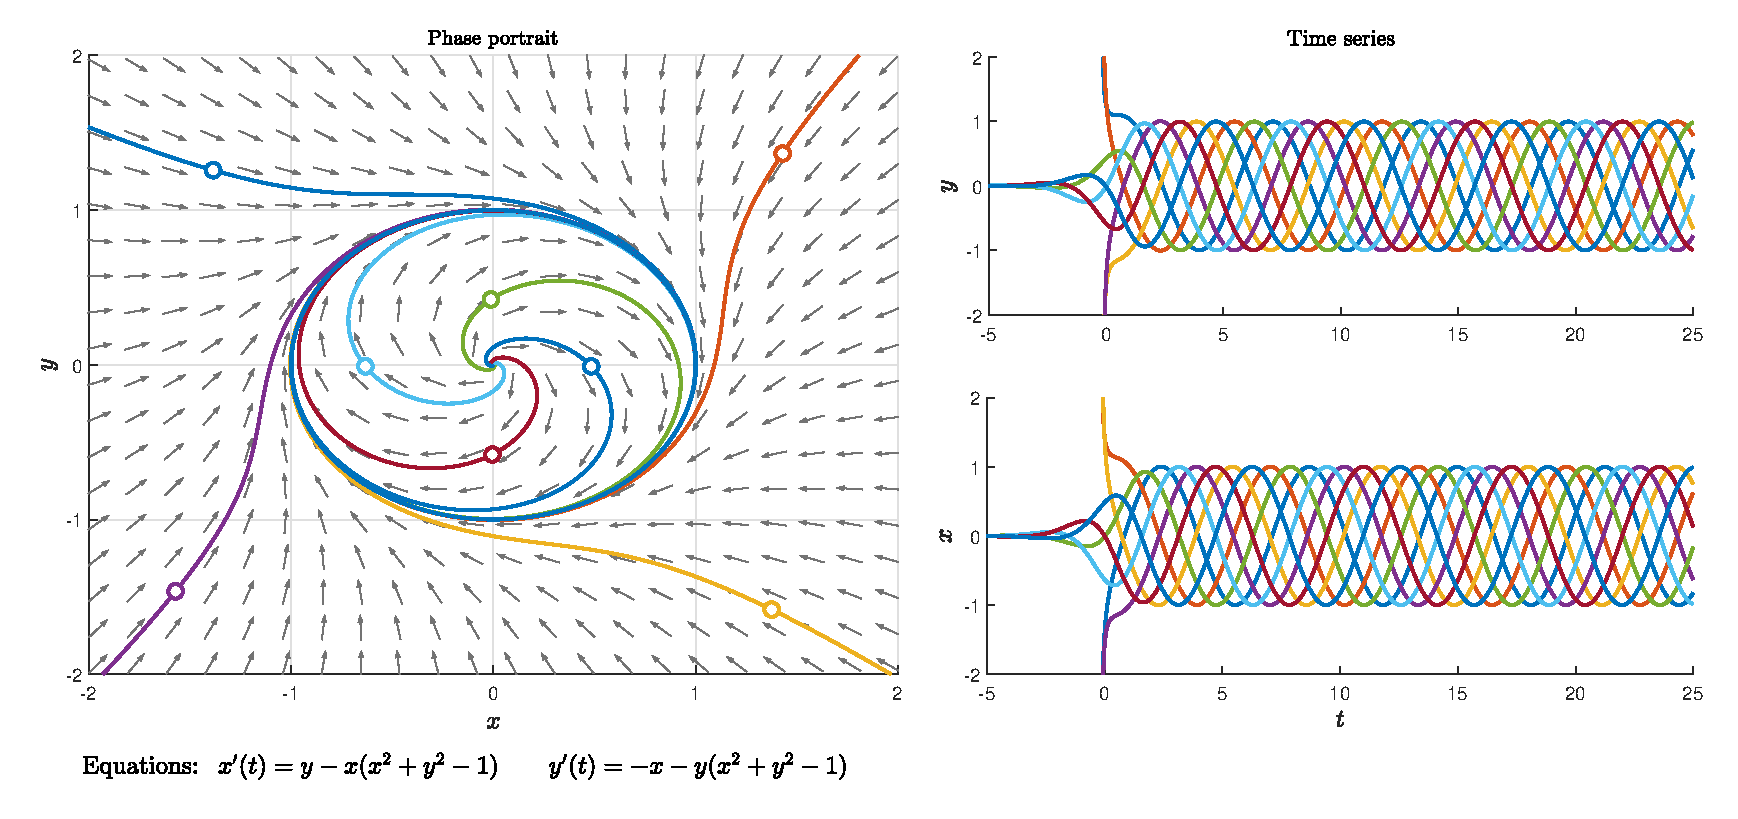
\includegraphics[width=1\textwidth]{cle.eps}
			\caption{Ciclo-Límite Asintóticamente Estable con sentido horario de giro}
			\label{fig:cle}
		\end{figure}\smallskip

	\newpage
		
	{\Large\textbullet\quad Ciclo-Límite Asintóticamente Inestable}\\[0.5cm]
	
	Si elegimos las condiciones iniciales dentro del Ciclo-Límite, las curvas solución tienden a cero. Si elegimos las condiciones iniciales fuera del Ciclo-Límite, las curvas solución tienden a infinito.
	
	\begin{figure}[h]
		\centering
		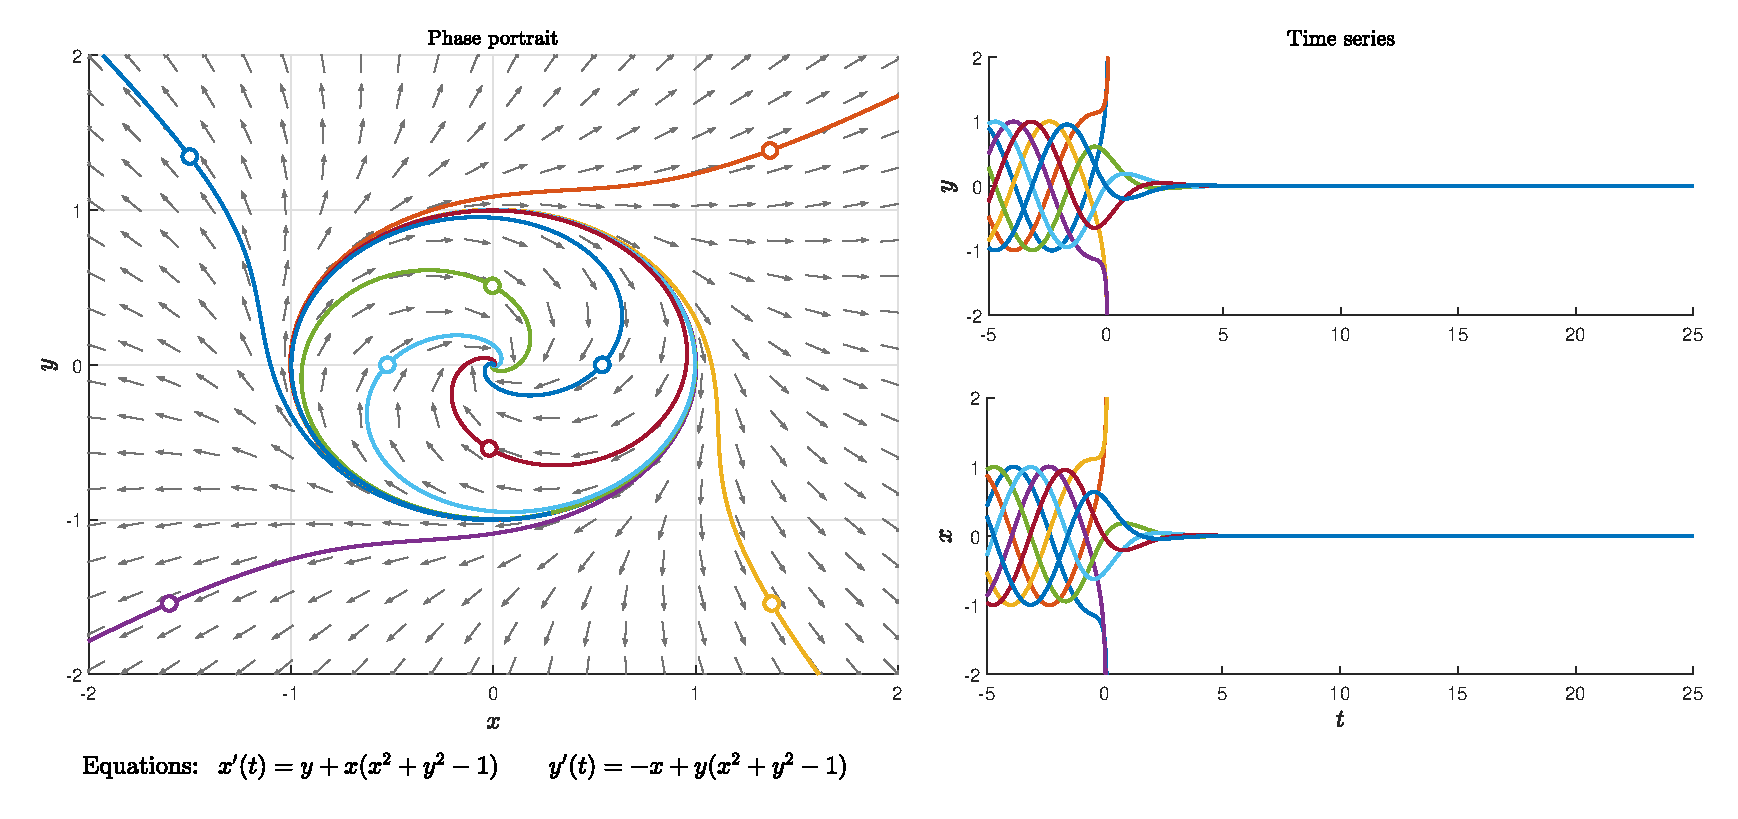
\includegraphics[width=1\textwidth]{cli.eps}
		\caption{Ciclo-Límite Asintóticamente Inestable con sentido horario de giro}
		\label{fig:cli}
	\end{figure}\smallskip
	
	\vspace{0.5cm}{\Large\textbullet\quad Ciclo-Límite Semi Asintóticamente Estable}\\[0.5cm]
	
	Si elegimos las condiciones iniciales dentro del Ciclo-Límite, las curvas solución tienden a cero. Si elegimos las condiciones iniciales fuera del Ciclo-Límite, las curvas solución tienden al Ciclo-Límite.
	
	\begin{figure}[h]
		\centering
		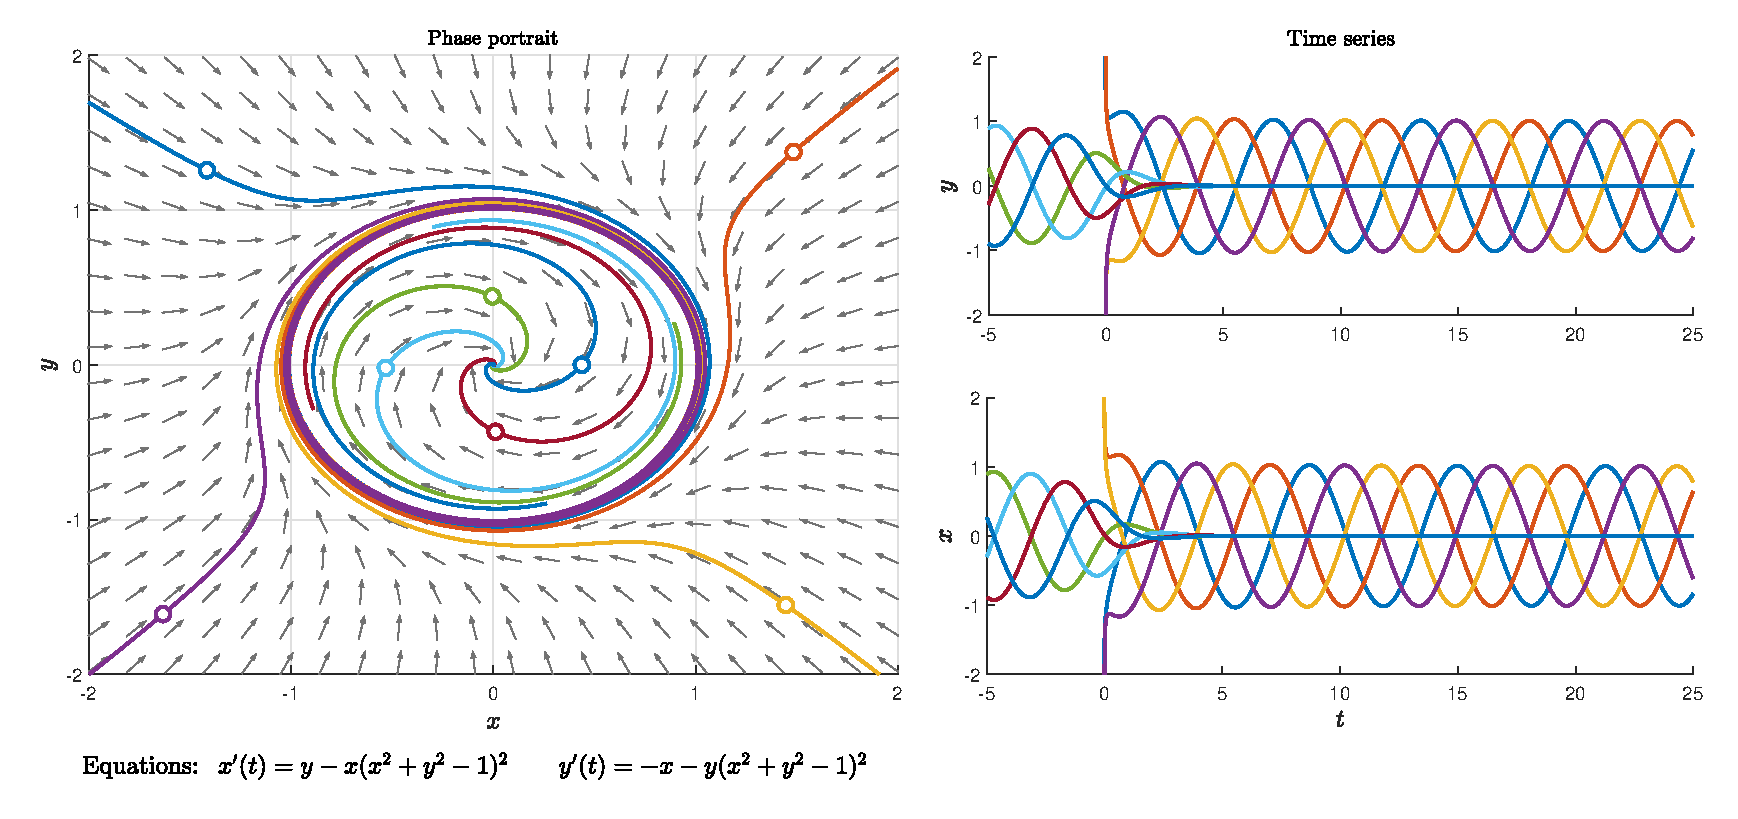
\includegraphics[width=1\textwidth]{clpe.eps}
		\caption{Ciclo-Límite Semi Asintóticamente Estable con sentido horario de giro}
		\label{fig:clpe}
	\end{figure}\smallskip
	\newpage
	
	El Ciclo-Límite que más nos interesa es el estable, ya que sin importar donde eligamos las condiciones iniciales siempre tenderemos a la oscilación periódica, además, si nuestro sistema sufre alguna perturbación que lo saque de la oscilación periódica siempre tenderá a reconducirse nuevamente hacia ella.
	
	\newpage
	
	\section{Bifurcación Foco-Centro-Ciclo Límite y su\\ cálculo mediante desarrollo en series.}
	
	\vspace{0.5cm}El estudio de los Ciclos-Límites historicamente se ha hecho de manera particular para cada sistema, primero hay que estudiar el punto de equilibrio y su estabilidad, hacer el análisis para saber si existe oscilación periódica y finalmente comprobar que dicha oscilación periódica esté aislada, lo cual no es nada sencillo. En nuestro caso no hará falta que hagamos este tipo de estudio gracias a que hemos sido capaces de escribir nuestro sistema \eref{eq:sistema1} de la manera \eref{eq:sis2ec} y este último en la forma \eref{eq:lienardrl} por lo que ya tenemos trabajos donde se hace este análisis para sistemas de este tipo y se corrobora la existencia de la bifurcación Foco-Centro-Ciclo Límite en los mismos, ver: \cite{ponce}, el Capítulo que inicia en la página 335 de \cite{ciclolimite} y las Secciones 8.1 y 3.6 de \cite{amarillo}, en concreto de este último el Teorema 3.27. En los anteriores trabajos se hace un análisis tradicional del problema, nosotros para ello haremos uso de la Caracterización integral que ya hemos visto, pero vamos a utilizar algunos conceptos que se ven en dichos trabajos, conceptos como la elección de un parámetro de bifurcación, puntos de equilibrios virtuales y requisitos que deben tener los parámetros del sistema. Cumpliendo esta serie de requisitos en los parámetros del sistema, los cuales veremos mas adelante, podemos conseguir que se produzca el cambio de estabilidiad Foco Asintóticamente Estable-Centro-Foco Asintóticamente Inestable en el punto de equilibrio del sistema y por ello obteniendo el Ciclo-Límite (ya que se produce la bifurcación Foco-Centro-Ciclo Límite), que será nuestra oscilación periódica.
	
	\newpage
	
	\vspace{0.5cm} Vamos a reescribir el Teorema 3.27 de \cite{amarillo} pero adaptando la nomenclatura a la de nuestro estudio
	
	\begin{theorem}
		\label{teo:5.1}
		Considerando el sistema \eref{eq:lienardrl}, donde tomamos $T_L$ como parámetro de bifurcación (esto es, suponemos que el resto de parámetros permanecen fijos), elegimos $a<0$ y $D_L>0$. El sistema experimenta una bifurcación Foco-Centro-Ciclo Límite al pasar $T_L$ por el valor cero. Es decir, de la configuración de Centro para $T_L=0$,ver \fref{fig:centro2}, se produce un Ciclo-Límite (que nace de la órbita periódica del Centro que es tangente a la sección de Poincarè) cuando $T_L T_R<0$ y $\mid T_L \mid$ es lo suficientemente pequeño. El Ciclo-Límite que nace es Asintóticamente Estable si $T_L>0$, ver \fref{fig:cle}, e Inestable cuando $T_L<0$, ver \fref{fig:cli}.
	\end{theorem}
	
	Veamos las condiciones para que se deben cumplir en nuestras ecuaciones y sus consecuencias para que se cumpla el Teorema \ref{teo:5.1} en nuestro sistema \eref{eq:lienardrl}:
		\begin{itemize}
			\item $a_R=a_L=a<0$ para que el punto de equilibrio de la zona Izquierda esté contenido en la zona $x<0$, ver \fref{fig:punto}, y que el posible punto de equilibrio de la zona Derecha tambien lo esté (punto de quilibrio virtual).
			\item Ya que $a_L<0$ y queremos que el polinomio característico  tenga raices imaginarias para tener una configuración de foco en nuestro punto de equilibrio, debemos tener $D_L>0$, ver \eref{eq:eqizq} y \eref{eq:eqpointL}.
			\item Como hemos establecido $a_R<0$, el posible punto de equilibrio de la zona Derecha estaría ubicado en la zona $x<0$, ver \eref{eq:eqpointR}, por ello podemos elegir:\begin{itemize}
				\item No hay punto de equilibrio $\rightarrow D_R=0$ 
				\item Si hay punto de equilibrio y es virtual $\rightarrow D_R\neq0$ 
			\end{itemize}

			\item Nuestro parámetro de bifurcación será $T_L$, por ello lo haremos variar de negativo a positivo haciendolo pasar por cero, $T_L<0 \rightarrow T_L=0 \rightarrow T_L>0$ y siempre para un valor pequeño de $\mid T_L \mid$. Lo hacemos de esta manera para que el Ciclo-Límite que obtengamos sea Estable y no Inestable
			\item Tenemos que $T_LT_R<0$ con $T_L>0$, por ello  $T_R<0$.
		\end{itemize}
		
		
	\vspace{0.5cm} En las siguientes figuras veremos gráficamente como se produce la bifurcacion tomando como parámetro de control $T_L$.
		
	\newpage
	
	\begin{figure}[h]
		\centering
		\includegraphics[width=1\textwidth]{foco3.jpg}
		\caption{Foco Asintóticamente Estable con sentido antihorario de giro y con la Sección de Poincaré en $x=-1$}
		\label{fig:foco3}
	\end{figure}\smallskip
	
	\newpage
	
	\begin{figure}[h]
		\centering
		\includegraphics[width=1\textwidth]{centro2.jpg}
		\caption{Centro con sentido con sentido antihorario de giro y con la Sección de Poincaré en $x=-1$}
		\label{fig:centro2}
	\end{figure}\smallskip
	
	\newpage
	
	\begin{figure}[h]
		\centering
		\includegraphics[width=1\textwidth]{ciclolimite3.jpg}
		\caption{Ciclo-Límite Asintóticamente Estable con sentido antihorario de giro y con la Sección de Poincaré en $x=-1$}
		\label{fig:ciclolimite3}
	\end{figure}\smallskip
	
	\newpage
	
	Para la demostración del Teorema \ref{teo:5.1} haremos uso principalmente de la Caracterización Integral de la semiaplicación de Poincaré, los desarrollos en series de MacLaurin y el Teorema de la Función Implícita, este último aún no lo hemos presentado.
	
	\begin{theorem}[Función Implícita]
		\label{teo.fi}
		Supongamos que $f:\mathbb{R}^2 \longrightarrow\mathbb{R}$ cuyas derivadas parciales existen y son continuas, con $f(x_0,y_0)=0$.\\[0.2cm]
		Si $\partial f / \partial y\neq0$, entonces existe una función $g$ definida en un intervalo abierto $I$ que contiene a $x_0$, de forma que $y_0=g(x_0)$ y además
		
		\begin{equation*}
			\scalebox{1.2}{$\displaystyle
			f(x,g(x))=0 \qquad \forall \: x\in I
			$}
		\end{equation*}\smallskip
		
		\noindent Es más, $g$ es derivable y con derivada continua en $I$.
		
	\end{theorem}
	
	\vspace{0.5cm}Ahora veremos la demostración del Teorema \ref{teo:5.1} \textcolor{red}{reescribir, por que realmente no vemos la demostracion completa paso a paso}
	\begin{proof}[\textbf{Demostración}]
		\label{dem5.1}
	Supongamos que nuestro sistema \eref{eq:lienardrl} posee una órbita periódica como la de la \fref{fig:aplipoincareL-Rcerrado}, queremos calcular los puntos $y_0, y_1$ que cierren dicha órbita, para ello haremos uso de la semiaplicación Izquierda y Derecha, \eref{eq:caracl}-\eref{eq:caracr}. Si la órbita es cerrada  y continua podemos formar el sistema \textcolor{red}{enfatizar en lo de la continuidad, cuando hablo de que todo este estudio es para un desarrollo local? al final cuando ya haya usado los desarrollos en series y el teorema de la funcion implicita?}
	
	\begin{equation}
		\label{eq:cierre}
		\scalebox{1.2}{$\displaystyle
			\left\{
			\begin{aligned}
				PV\left\{\int_{y_1}^{y_0}\frac{-y}{D_Ly^2-aT_Ly+a^2}dy\right\}&=\frac{k_L\pi T_L}{D_L\sqrt{4D_L-T_L^2}}
				\\[2mm]
				PV\left\{\int_{y_1}^{y_0}\frac{-y}{D_Ry^2-aT_Ry+a^2}dy\right\}&=\frac{-k_R\pi T_R}{D_L\sqrt{4D_L-T_L^2}}
			\end{aligned}
			\right. 
			$}
	\end{equation}\smallskip
	
	Recordemos del Teorema \ref{teo:5.1} que son son constantes en nuestro sistema $D_L,D_R,a,k_L,k_R,T_R$, con $a<0$ por lo que $k_L$ y $k_R$ serían $k_L=2$ y $k_R=0$. Luego, en \eref{eq:cierre} tenemos
	
	\begin{equation}
		\label{eq:cierre2}
		\scalebox{1.2}{$\displaystyle
			\left\{
			\begin{aligned}
				&\int_{y_1}^{y_0}\frac{-y}{D_Ly^2-aT_Ly+a^2}dy-\frac{k_L\pi T_L}{D_L\sqrt{4D_L-T_L^2}}&=0
				\\[2mm]
				&\int_{y_1}^{y_0}\frac{-y}{D_Ry^2-aT_Ry+a^2}dy&=0
			\end{aligned}
			\right. 
			$}
	\end{equation}\smallskip
	
	\begin{equation}
		\label{eq:cierre3}
		\scalebox{1.2}{$\displaystyle
			\left\{
			\begin{aligned}
				&F_1(y_0,y_1,T_L)&=0
				\\[2mm]
				&F_1(y_0,y_1)&=0
			\end{aligned}
			\right. 
			$}
	\end{equation}\smallskip
	
	\vspace{0.5cm}\noindent En \eref{eq:cierre3} tenemos un sistema de 2 ecuaciones con 3 incógnitas, por lo que el objetivo será llegar a un sistema de 2 ecuaciones con dos incógnitas, $y_0$ y $T_L$. Para ello primero definiremos $y_1=f_2(y_0)$ y luego $y_0=f_1(T_L)$. Parte de este procedimiento se realiza en \cite{properties}, debido a su extensión y complejidad queda fuera de los márgenes de este trabajo, por ello vamos a exponer los resultados directamente 
	
	\vspace{0.5cm}Como se ha dicho el primer objetivo es pasar de $F_2=(y_0,y_1) \longrightarrow y_1=f_2(y_0)$. Esto se realiza en la Proposición 3.1 de \cite{properties} mediante un desarrollo en series de MacLaurin, obtendiendose:
	
		\begin{equation}
		\label{eq:macla}
		\scalebox{1.2}{$\displaystyle
			y_1=-y_0-\frac{2T_R}{3a}y_0^2-\frac{4T_R^2}{9a^2}y_0^3+...
			$}
	\end{equation}\smallskip
	
	\vspace{0.5cm}\noindent Ahora podemos escribir la primera expresion de \eref{eq:cierre2} de la siguente manera
	
	\begin{equation}
		\label{eq:macla2}
		\scalebox{1.2}{$\displaystyle
			\begin{gathered}
				\int_{-y_0-\frac{2T_R}{3a}y_0^2+...}^{y_0}\frac{-y}{D_Ly^2-aT_Ly+a^2}dy-\frac{k_L\pi T_L}{D_L\sqrt{4D_L-T_L^2}}=0\\[3mm]
				\tilde{F}_1(y_0,T_L)=0
			\end{gathered}	
			$}
	\end{equation}

	\vspace{0.5cm} Comprobemos haciendo uso del Teorema \ref{teo.fi} si existe de manera local alguna función que nos permita definir $y_0=f_1(T_L)$. Cuando se realizan las derivadas parciales de $\tilde{F}_1(y_0,T_L)=0$ obtenemos:
	
	\begin{equation}
		\label{dpar}
		\frac{\partial F_1}{\partial y_0}=0 \qquad \text{y} \qquad \frac{\partial F_1}{\partial T_L}=\frac{k_L\pi}{2D_L^{3/2}}
	\end{equation}\smallskip
	
	\vspace{0.5cm}\noindent Como la derivada parcial de la función $\tilde{F}_1$ respecto $y_0$ es cero no podemos expresar $y_0=f_1(T_L)$, pero como la derivada parcial de la función $\tilde{F}_1$ respecto $T_L$ es distinto de cero, eso significa que existe una única función que nos permite definir $T_L=f_1(y_0)$ de manera local. Esta función se puede calcular haciendo un desarrollo en series de MacLaurin de \eref{eq:macla2}, obteniéndose:
	
	\begin{equation}
		\label{macla3}
		T_L=\frac{2\, D_L^{3/2}\, T_R}{3\, a_L^2\, a_R \, \pi}\: y_0^3+\frac{2\, D_L^{3/2}\, T_R^2}{9\, a_L^2\, a_R^2 \, \pi}\: y_0^4-...
	\end{equation}\smallskip
	
	\vspace{0.5cm}\noindent Realizando una inversión de la serie  anterior podemos finalmente definir $y_0=f_1(T_L)$:
	
	\begin{equation}
		\label{eq:macla4}
		\begin{aligned}
		&y_0^3\backsimeq \left( \frac{3\, a_L^2\, a_R \, \pi}{2\, D_L^{3/2}\, T_R} \right)\cdot \left(T_L\right)+...\\[3mm]
		&y_0\backsimeq \left( \frac{3\, a_L^2\, a_R \, \pi}{2\, D_L^{3/2}\, T_R} \right)^{1/3}\cdot \left(T_L\right)^{1/3}+... \qquad \text{para} \quad T_R \neq 0
	\end{aligned}
	\end{equation}
	
	\vspace{0.5cm}Las expresiones \eref{eq:macla} y \eref{eq:macla4} son las que usaremos más adelante para calcular los puntos $y_0,y_1$. Con esto queda finalizada la Demostración \ref{dem5.1}.
	
	\end{proof}
	
	\vspace{0.5cm}Se puede calcular el periodo de la oscilación mediante la obtención de los semitiempos de vuelo izquierdo y derecho, nuevamente la obtención de estas expresiones se escapa de los objetivos de este trabajo por lo que  únicamente las presentaremos. Se puede consultar el Teorema 19 de \cite{caracterizacion} para profundizar más en este apartado.
	
	\vspace{0.5cm} Definiremos el periodo de la oscilación $T_P$ como la suma del semitiempo de vuelo izquierdo $\tau_L$ y el semitiempo de vuelo derecho $\tau_R$. A continuación veremos las expresiones de los semitiempos de vuelo prsentadas en \cite{caracterizacion}.
	
	\vspace{0.5cm}\noindent Semitiempo de vuelo izquierdo
	
	\begin{equation}
		\label{eq:semitiempoL}
		\scalebox{1.2}{$\displaystyle
		\tau_L=\frac{4\pi}{D_L\sqrt{4D_L^2-T_L^2}}+\int_{y_1}^{y_0}\frac{a_L}{D_Ly^2-aT_Ly+a^2}dy
		$}
	\end{equation}\smallskip
	
	\vspace{0.5cm}\noindent Semitiempo de vuelo derecho
	
	\begin{equation}
		\label{eq:semitiempoR}
		\scalebox{1.2}{$\displaystyle
		\tau_R=\int_{y_1}^{y_0}\frac{-a_R}{D_Ry^2-aT_Ry+a^2}dy
		$}
	\end{equation}\smallskip
	
	\vspace{0.5cm} Recordemos que tenemos fijos los parámetros $D_L,D_R,a,T_R$, por lo que las anteriores expresiones \eref{eq:semitiempoL}-\eref{eq:semitiempoR} dependen únicamente de $y_0$ e $y_1$. Como ya hemos visto en la Demostración \ref{dem5.1} podemos escribir $y_1=f(y_0)$ e $y_0=f(T_L)$, por lo que las expresiones \eref{eq:semitiempoL}-\eref{eq:semitiempoR} tan solo dependerán de $T_L$. A continuación presentaremos el desarrollo en series que hemos calculado para cada semitiempo de vuelo, donde hemos sustitudo $y_1$ por la expresión en función de $y_0$ que vimos en \eref{eq:macla}:
	
	\begin{equation}
		\label{eq:seriestL}
		\tau_L=\frac{4\pi}{D_L\sqrt{4D_L^2-T_L^2}}+\frac{2y_0}{a_L}-\frac{2T_Ry_0^2}{3a_La_R}+\frac{(4a_L^2T_R^2+6a_R(a_LT_RT_L+a_R(-D_L+T_L^2)))y_0^3}{9a_R^2a_L^3}
	\end{equation}\smallskip
	
	\vspace{0.5cm}
	
	\begin{equation}
		\label{eq:seriestR}
		\tau_R=-\frac{2y_0}{a_R}+\frac{2T_Ry_0^2}{3a_R^2}+\frac{2(3D_R-8T_R^2)y_0^3}{9a_R^3}
	\end{equation}\smallskip
	
	\vspace{0.5cm}\noindent Sumando los semitiempos anteriores obtenemos el periodo:
	
	\begin{equation}
		T_P=\tau_L + \tau_R = \frac{4\pi}{D_L\sqrt{4D_L^2-T_L^2}}+\frac{2(D_R-D_L-2T_R^2+T_RT_L+T_L^2)y_0^3}{a_L^3}
	\end{equation}
	
	\newpage
	
	\chapter{Oscilación Peródica en el circuito}
	
	Ya hemos visto las herramientas matemáticas necesarias, la forma en que debemos describir nuestro circuito y las condiciones para obtener la bifurcación que nos proporcione la oscilación periódica que estamos buscando, en este capítulo se va a poner todo ello en práctica.
	
	\vspace{0.5cm} Lo primero es obtener las ecuaciones diferenciales del circuito y decicir cuáles serán nuestras variables de estado, esto se hizo en \eref{eq:kir111}-\eref{eq:kir222}-\eref{eq:kir333} y se establecieron como variables de estado:
	
	\begin{itemize}
		\item Tensión en el condensador y el memristor: \bm{$x=v_1$}
		\item Intensidad en la bobina y la resistencia negativa: \bm{$y=i_{LR}$}
		\item Flujo en el memristor: \bm{$z=\varphi$}
	\end{itemize}
	
	\vspace{0.5cm} Seguidamente se reordenan los coeficientes del anterior sistema para poder trabajar mas comodamente, llegando al sistema tridimendional \eref{eq:sistema}, con la función $W(z)$ \eref{eq:wz}.
	
	\vspace{0.5cm} A continuación, gracias a las superficies invariantes \eref{eq:sh} existentes en el sistema, podemos pasar de estudiar el sistema tridimensional \eref{eq:sistema} a uno equivalente bidimesional trizonal en forma canónica de Lienard \eref{eq:sis2ec}, con las rectas de separación en $x=\pm1$.
	
	\vspace{0.5cm} De este último sistema trizonal \eref{eq:sis2ec} nos fiajaremos únicamente en dos de sus zonas, ya que la oscilación que se está tratando de obtener es bizonal, por lo que nos fijaremos por ejemplo en las zonas a la izquierda y a la derecha de la recta de separación $x=-1$.
	
	\begin{equation}
		\label{eq:sisbiz}
		\begin{gathered}
			\left\{
			\begin{aligned}
				\dot{x}&=t_E(x+1)-t_C-y
				\\[2mm]
				\dot{y}&=d_E(x+1)-d_C-h
			\end{aligned}
			\right. \qquad 
			\rule[-40pt]{1.5pt}{80pt} \qquad 
			\left\{
			\begin{aligned}
				\dot{x}&=t_Cx-y
				\\[2mm]
				\dot{y}&=d_Cx-h
			\end{aligned}
			\right. \\ \quad\qquad\qquad x=-1
		\end{gathered}
	\end{equation}\smallskip
	
	 \vspace{0.5cm}\noindent Pero antes de continuar debemos hacer una translación de la recta de separación $x=-1$ a la recta $x=0$ ya que esta es una condición fundamental para el resto de herramientas que hemos presentado.
	
	\newpage
	
	\vspace{0.5cm}\noindent Aplicaremos a \eref{eq:sisbiz} el primer cambio de variable:
	
	\begin{equation}
		\label{eq:cambioo1}
		X=x+1 \quad \longrightarrow \quad x=X-1 \quad \textit{y} \quad \dot{X}=x
	\end{equation}
	
	\begin{equation}
		\label{eq:cb1}
		\begin{gathered}
			\left\{
			\begin{aligned}
				\dot{X}&=t_EX-t_C-y
				\\[2mm]
				\dot{y}&=d_EX-d_C-h
			\end{aligned}
			\right. \qquad 
			\rule[-40pt]{1.5pt}{80pt} \qquad 
			\left\{
			\begin{aligned}
				\dot{X}&=t_CX-t_C-y
				\\[2mm]
				\dot{y}&=d_CX-d_C-h
			\end{aligned}
			\right. \\  \!\! X=0
		\end{gathered}
	\end{equation}\smallskip
	
	\vspace{0.5cm}\noindent Aplicaremos a \eref{eq:cb1} el segundo cambio de variable:
	
	\begin{equation}
		\label{eq:cambioo2}
		Y=y+t_C \quad \longrightarrow \quad y=Y-t_C \quad \textit{e} \quad \dot{Y}=y
	\end{equation}
	
	\begin{equation}
		\label{eq:cb2}
		\begin{gathered}
			\left\{
			\begin{aligned}
				\dot{X}&=t_EX-Y
				\\[2mm]
				\dot{Y}&=d_EX-d_C-h
			\end{aligned}
			\right. \qquad 
			\rule[-40pt]{1.5pt}{80pt} \qquad 
			\left\{
			\begin{aligned}
				\dot{X}&=t_CX-Y
				\\[2mm]
				\dot{Y}&=d_CX-d_C-h
			\end{aligned}
			\right. \\  \!\! X=0
		\end{gathered}
	\end{equation}\smallskip
	
	\vspace{0.5cm}\noindent Por lo que tenemos
	
	\begin{equation}
		\label{eq:cb3}
		\begin{gathered}
			\begin{pmatrix*}[r]
				\dot{X}\\ \dot{Y}
			\end{pmatrix*}= \begin{pmatrix*}[r]
				t_E & -1 \\ d_E & 0
			\end{pmatrix*} \begin{pmatrix*}[r]
				X \\ Y
			\end{pmatrix*}-\begin{pmatrix*}[c]
				0 \\ d_C+h
			\end{pmatrix*} \qquad 
			\rule[-40pt]{1.5pt}{80pt} \qquad 
				\begin{pmatrix*}[r]
				\dot{X}\\ \dot{Y}
			\end{pmatrix*}= \begin{pmatrix*}[r]
				t_C & -1 \\ d_C & 0
			\end{pmatrix*} \begin{pmatrix*}[r]
				X \\ Y
			\end{pmatrix*}-\begin{pmatrix*}[c]
				0 \\ d_C+h
			\end{pmatrix*} \\ X=\;0
		\end{gathered}
	\end{equation}\smallskip
	
	\newpage
	
	\vspace{0.5cm} \noindent Como se puede comprobar el sistema \eref{eq:cb3} es equivalente al sistema en forma canónica de Liènard \eref{eq:lienardrl} que vimos a final de la Sección \ref{sistrobiz}, por lo que todo el análisis posterior que hicimos para un sistema tipo \eref{eq:lienardrl} lo podremos aplicar a nuestro sistema \eref{eq:cb3}. Los parámetros del sistema en relación a nuestro circuito son
	
	\begin{equation}
		\label{eq:misistema}
			\scalebox{1.2}{$\displaystyle
		\begin{aligned}
			&T_L=t_E = b \cdot a_{11} + a_{22} = \frac{-b}{C}+\frac{R}{L} \\[3mm]
			&D_L=d_E = b \cdot a_{11}a_{22} - a_{21}a_{12} = \frac{-b}{C}\frac{R}{L}-\frac{-1}{L}\frac{1}{C}=\frac{-bR}{CL}+\frac{1}{CL} \\[3mm]
			&T_R=t_C = a \cdot a_{11} + a_{22} = \frac{-a}{C}+\frac{R}{L} \\[3mm]
			&D_R=d_C = a \cdot a_{11}a_{22} - a_{21}a_{12} = \frac{-a}{C}\frac{R}{L}-\frac{-1}{L}\frac{1}{C}=\frac{-aR}{CL}+\frac{1}{CL}\\[3mm]
			&a=d_C+h = a \cdot a_{11}a_{22} - a_{21}a_{12}+h= \frac{-aR}{CL}+\frac{1}{CL}+h
		\end{aligned}
		$}
	\end{equation}
	
	\newpage
	
	 El siguiente paso es recordar las condiciones que se estudiaron en el Teorema \ref{teo:5.1} para que se produzca la bifurcación Foco-Centro-Ciclo Límite y ajustar dichas condiciones con un parámetro del circuito, este será la resistencia negativa. Es decir, modificando la resistencia del circuito haremos que se produzca el cambio en la traza y por tanto el cambio en la estabilidad del punto de equilibrio.
	
	\vspace{0.5cm}{\large\textbullet\quad Condición I}
	
	\begin{equation*}
		a=d_C+h<0 \quad \longrightarrow \quad \frac{-aR}{CL}+\frac{1}{CL}+h<0,
	\end{equation*}\smallskip
	\begin{empheq}[box=\fbox]{equation}
		\label{eq:cond1}
		R>\frac{1}{a}+\frac{CL}{a}\, h.
	\end{empheq}
	
	\vspace{1cm}{\large\textbullet\quad Condición II}
	
	\begin{equation*}
		D_L>0 \quad \longrightarrow \quad \frac{-bR}{CL}+\frac{1}{CL}>0,
	\end{equation*}\smallskip
	\begin{empheq}[box=\fbox]{equation}
		\label{eq:cond2}
		R<\frac{1}{b}.
	\end{empheq}
	
	\vspace{1cm}{\large\textbullet\quad Condición III}
	
	\begin{equation*}
		T_R<0 \quad \longrightarrow \quad \frac{-a}{C}+\frac{R}{L}<0,
	\end{equation*}\smallskip
	\begin{empheq}[box=\fbox]{equation}
		\label{eq:cond3}
		R<a \, \frac{L}{C}.
	\end{empheq}
	
	\vspace{1cm}{\large\textbullet\quad Condición IV}
	
	\begin{equation*}
		T_L=0 \quad \longrightarrow \quad \frac{-b}{C}+\frac{R}{L}=0,
	\end{equation*}\smallskip
	\begin{empheq}[box=\fbox]{equation}
		\label{eq:cond4}
		T_L\left\{
		\begin{aligned}
			>0 \qquad para \quad R>b \, \frac{L}{C}\\[3mm]
			=0 \qquad para \quad R=b \, \frac{L}{C}\\[3mm]
			<0 \qquad para \quad R<b \, \frac{L}{C}
		\end{aligned}
		\right.
	\end{empheq}
	
	\newpage
	
	Ahora ajustaremos los parámetros $a,b,h,R,L,C$ para que las cuatro condiciones anteriores se cumplan simultáneamente
	
	\vspace{0.5cm}\noindent De las condiciones III y IV obtenemos la relación entre $a$ y $b$:
	
	\begin{equation*}
		a \, \frac{L}{C}>R=b \, \frac{L}{C} \quad \longrightarrow \quad a>b
	\end{equation*}\smallskip
	\begin{equation}
		\label{c1f}
		\text{Elegiremos}\left\{
		\begin{aligned}
			&a=0.2\\[2mm]
			&b=0.01
		\end{aligned}
		\right.
	\end{equation}
	
	\vspace{0.5cm}\noindent Comprobemos la condición II:
	
	\begin{equation}
		\label{eq:c2f}
		R<\frac{1}{b}=\frac{1}{0.01} \quad \longrightarrow \quad R<100
	\end{equation}\smallskip
	
	\vspace{0.5cm}\noindent Ahora se establecerá el valor de $R$ límite, para que se produzca el cambio en la traza izquierda $T_L<0 \rightarrow T_L=0 \rightarrow T_L>0$, con la condición IV. Haremos que el cambio se produzca para $R=1$ y comprobaremos la relación entre $L$ y $C$ que obtendremos tras ello:
	
	\begin{equation*}
		\begin{aligned}
			\text{Establecemos} \quad &\longrightarrow \quad R=1 \\[2mm]
			\text{Condición IV} \quad &\longrightarrow \quad C=0.01L\\[2mm]
			\text{Elegiremos} \quad &\longrightarrow \quad C=100\cdot10^{-3}(F), \quad L=10(H).
		\end{aligned}
	\end{equation*}\smallskip
	
	\vspace{0.5cm}\noindent A continuación comprobemos la condición I para establecer el valor de $h$:
	
	\begin{equation*}
	\begin{gathered}
		R>\frac{1}{a}+\frac{CL}{a}\, h\\[3mm] R>\frac{1}{0.2}+\frac{100\cdot10^{-3}\cdot10}{0.2}\, h \\[3mm]
		R>5+5h \\[3mm]
		\text{Por lo que}\quad h<0, \qquad \text{Escogeremos}\quad h=-1.\\[3mm]
		R>5+5(-1)=0
	\end{gathered}
	\end{equation*}\smallskip
	
	\vspace{0.5cm}\noindent Por último comprobemos la condicion III:
	
	\begin{equation*}
		R<a \, \frac{L}{C} \quad \longrightarrow \quad R<0.2\:\frac{10}{100\cdot10^{-3}}=20
	\end{equation*}
	
	\newpage
	
	A modo de resumen, estos serán los valores elegidos para los parámetros de nuestro sistema \eref{eq:cb3}:
	
	\begin{itemize}
		\item $a=0.2$
		\item $b=0.01$
		\item $h=-1$
		\item $C=100\cdot10^{-3}\:(F)$
		\item $L=10\:(H)$
		\item $R\lesseqqgtr1\:(\Omega)$
	\end{itemize}
	
	\vspace{0.5cm}\noindent Se han elegido los anteriores valores para una mayor comodidad a la hora de hacer los cálculos pero obviamente no son valores comerciales de $R,L,C$. Si se quisiera implementar el circuito habría que realizar un trabajo más extenso con las inecuaciones anteriores para ajustar los parámetros a valores comerciales, además no se podría elegir libremente los valores de $a$ y $b$ ya que estos dependen de la curva característica flujo-carga del memristor.
	
	\vspace{0.5cm} A continuación pasemos a comprobar con MATLAB que efectivamente aparece el Ciclo-Límite en nuestro circuito con los valores anteriores.
	
	 \vspace{0.5cm}Calcularemos $y_0$ e $y_1$ con las expresiones \eref{eq:macla}-\eref{eq:macla4}. En la expresión \eref{eq:macla} donde apareca $y_0$ lo sustituiremos por \eref{eq:macla4}, de esta manera tendremos tanto $y_0$ como $y_1$ en función de $T_L$, esto lo haremos ya que como vimos en \eref{eq:misistema} podemos escribir $T_L=f(b,C,L,R)$ y ya dijimos anteriormente que solo variaremos $R$ del circuito, por lo que de esta manera conseguimos tener $y_0$, $y_1$ y $T_L$ en función de $R$.
	
	\newpage
	
	\lstinputlisting[style=Matlab-editor]{Ejemplo_4.m}
	
	\newpage
	
	\lstinputlisting[style=Matlab-bw]{cwejem4.m}
	
	\vspace{1cm}\noindent En la siguiente página veremos la gráfica obtenida de ``Ejemplo 4 TFE'' donde aparecen la gráfica de $Y_0$ e $Y_1$ en función de $R$ y la gráfica del periodo también en función de $R$.

\newpage

	\begin{figure}[h]
	\centering
	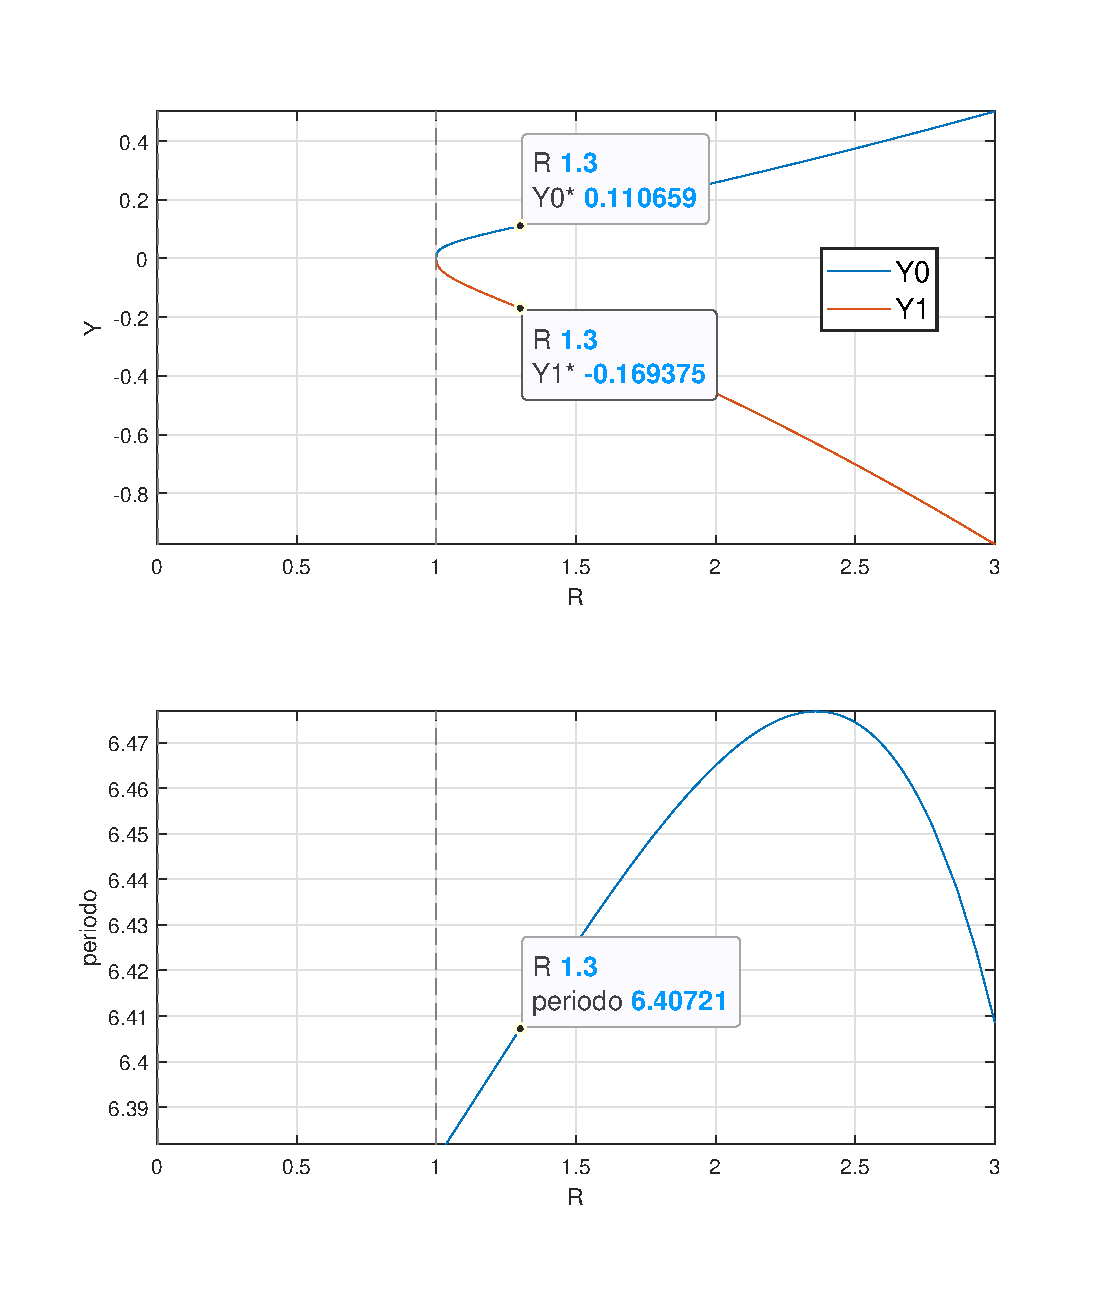
\includegraphics[width=1\textwidth]{ejem4.eps}
	\caption{Gráfica obtenida de ``Ejemplo 4 TFE''}
	\label{fig:ejem4}
	\end{figure}\smallskip
	
	\vspace{0.5cm}\noindent A continuación veremos una pequeña modificación del código ``Ejemplo 4'' para ver más ampliamente la gráfica de $Y_0$ e $Y_1$ en función de $R$ y así comprobar que se cumplen las condiciones que nos aparecieron al trabajar con las inecuaciones.
	
	\newpage
	
	\lstinputlisting[style=Matlab-editor]{Ejemplo_5.m}
	
	\newpage
	
	\begin{figure}[h]
		\centering
		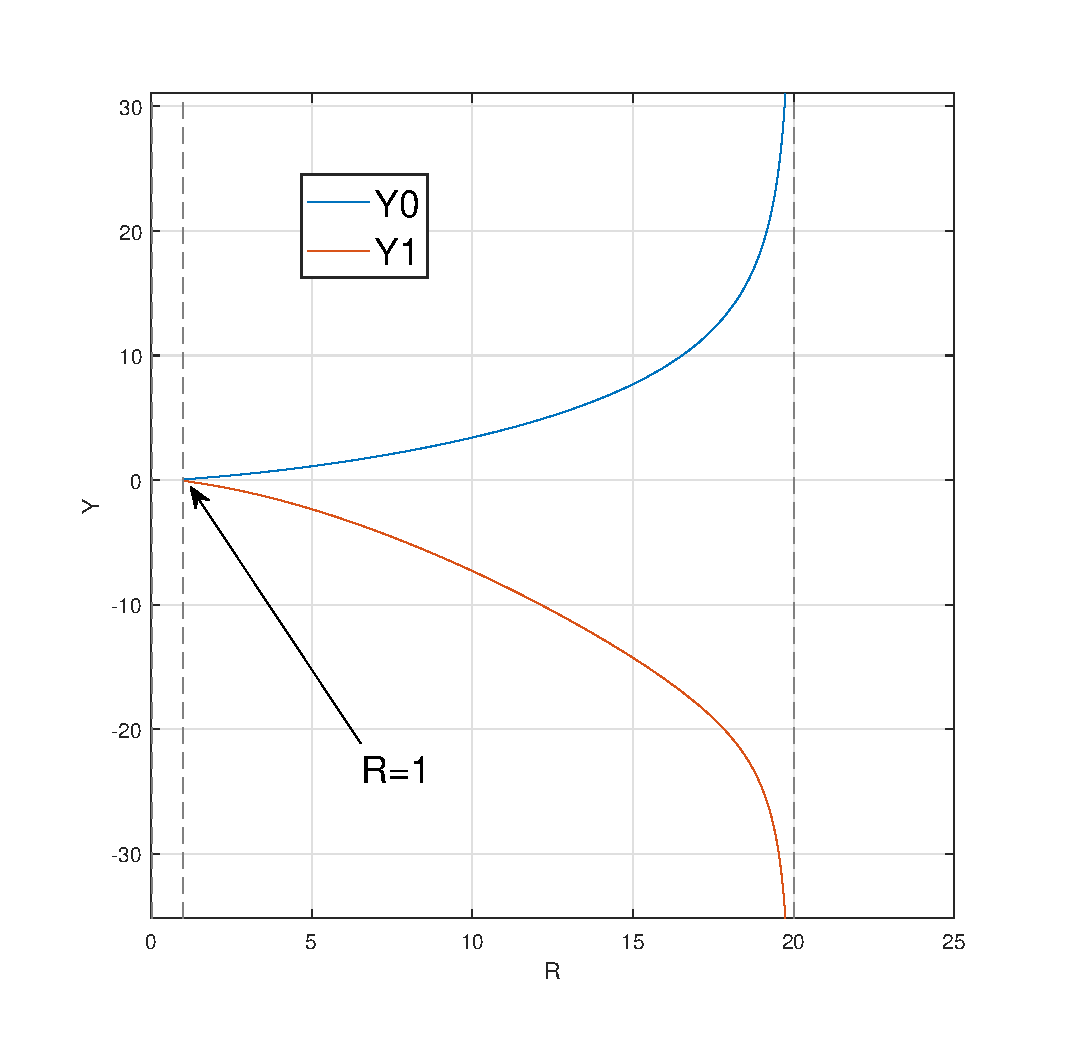
\includegraphics[width=1\textwidth]{ry1ry0.eps}
		\caption{Gráfica obtenida de ``Ejemplo 5''}
		\label{fig:ry1ry0}
	\end{figure}\smallskip
	
	\vspace{0.5cm}\noindent Como se puede comprobar en la \fref{fig:ry1ry0} se cumplen las condiciones que establecimos en la página \textcolor{red}{como referencio una página de mi propio trabajo?}, estas eran: $R<20$ y $R>1$ para que aparezca el Ciclo-Límite, es decir, se empiecen a obtener valores de corte $Y_0>0$ e $Y_1<0$ con la recta de separación $X=0$.
	
	\newpage
	
	Para finalizar el estudio vamos a ver gráficamente el Ciclo-Límite, para ello hay que reescribir el sistema \eref{eq:sis2ec} haciendo uso de los valores absolutos, la función de MATLAB que define funciones a trozos o la función signo como ya hicimos en \eref{eq:clejem}.
	
	\begin{equation}
		\label{eq:clejemsis}
		\scalebox{1.2}{$\displaystyle
			\left\{
			\begin{aligned}
				\dot{x}&=t_Ex-y+(t_C-t_E)\frac{1}{2}\left( \mid x+1 \mid - \mid x-1 \mid \right),
				\\[2mm]
				\dot{y}&=d_Ex+(d_C-d_E)\frac{1}{2}\left( \mid x+1 \mid - \mid x-1 \mid \right)-h.
			\end{aligned}
			\right. 
			$}
	\end{equation}\smallskip
	
	\vspace{0.5cm}Siendo $t_E,t_C,d_E,d_C$ los vistos en \eref{eq:misistema}, los cuales en siguiente código en MATLAB se han sustituido para dejar todos los parámetros en función de $R$.
	
	\begin{figure}[h]
		\centering
		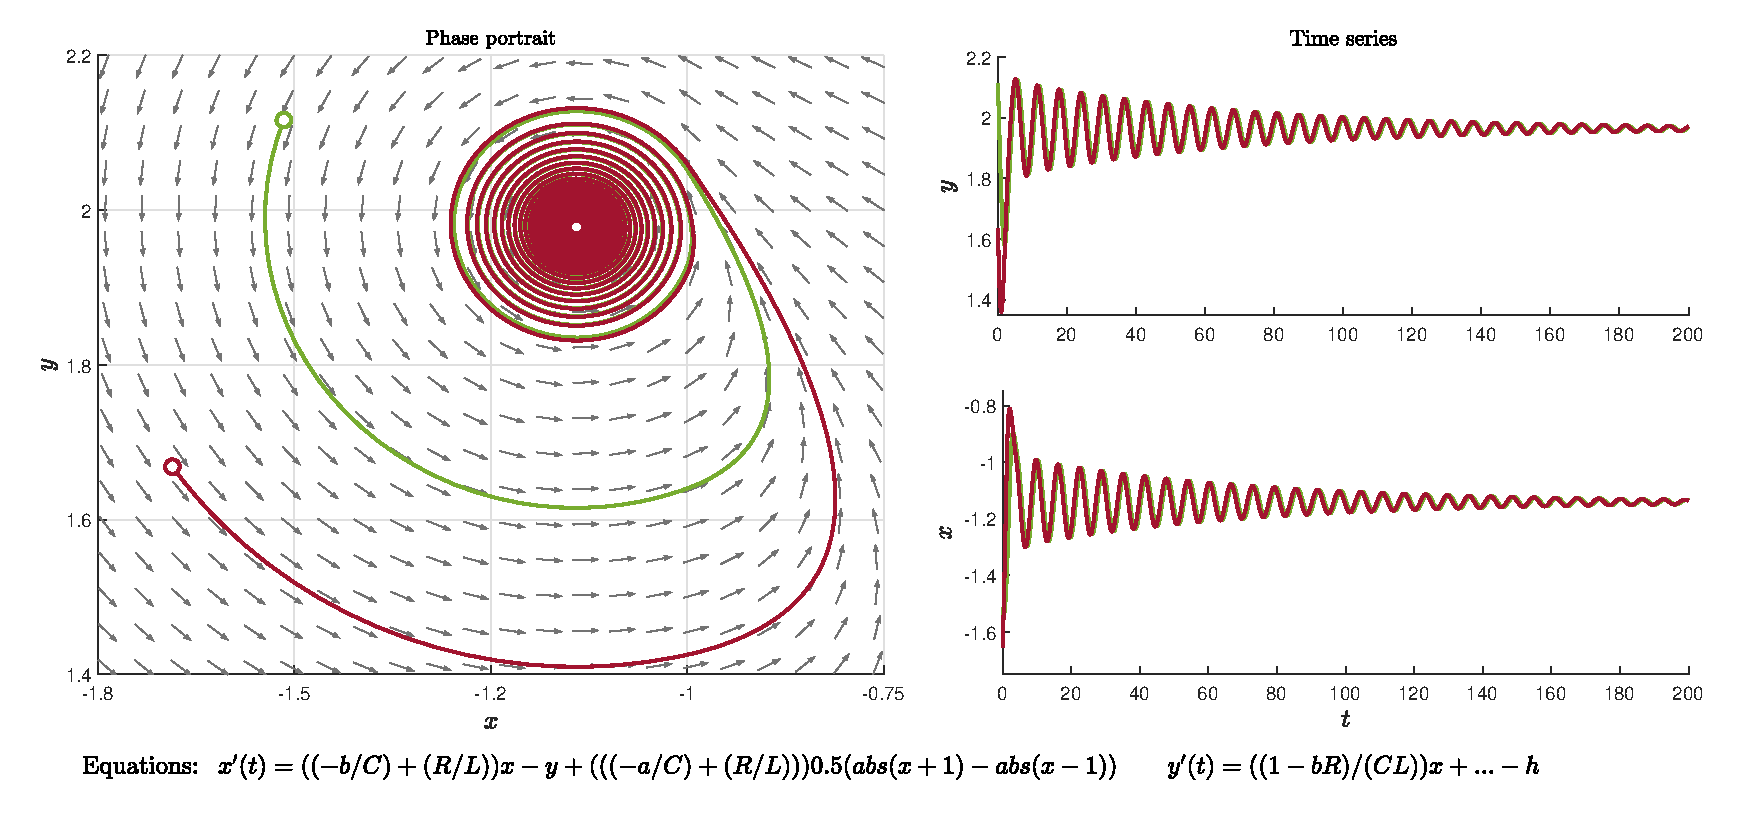
\includegraphics[width=1\textwidth]{r0.7.eps}
		\caption{Configuración de Foco Asintóticamente Estable para $R=0.7$}
		\label{fig:r0.7}
	\end{figure}
	\begin{figure}[h]
		\centering
		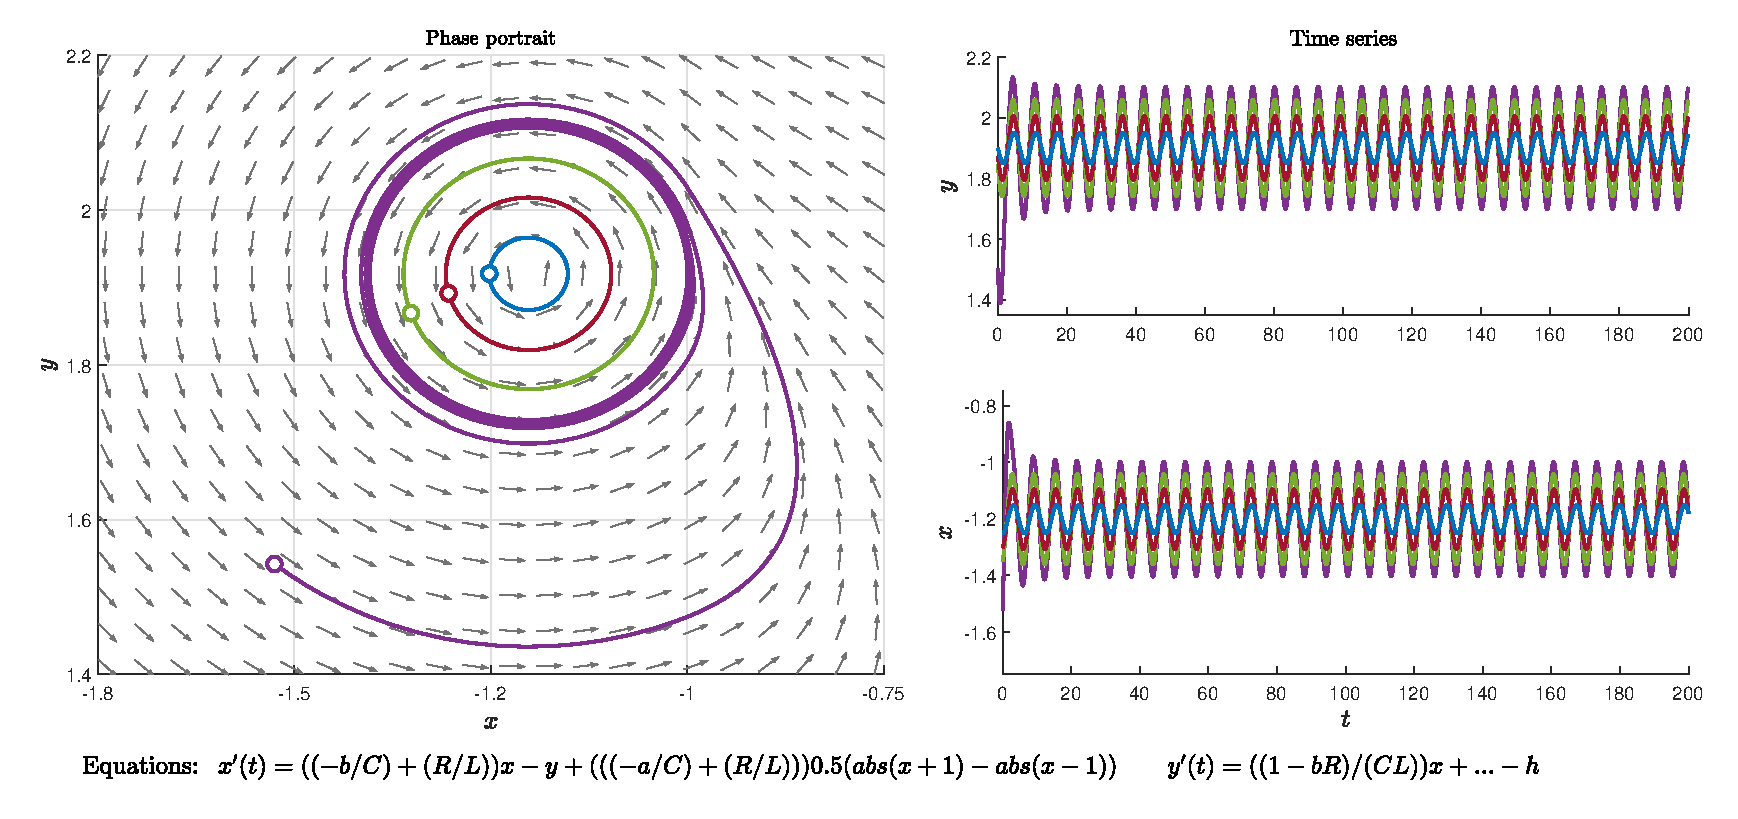
\includegraphics[width=1\textwidth]{r1.eps}
		\caption{Configuración de Centro para $R=1$}
		\label{fig:r1}
	\end{figure}
	
	\newpage
	
	\begin{figure}[h]
		\centering
		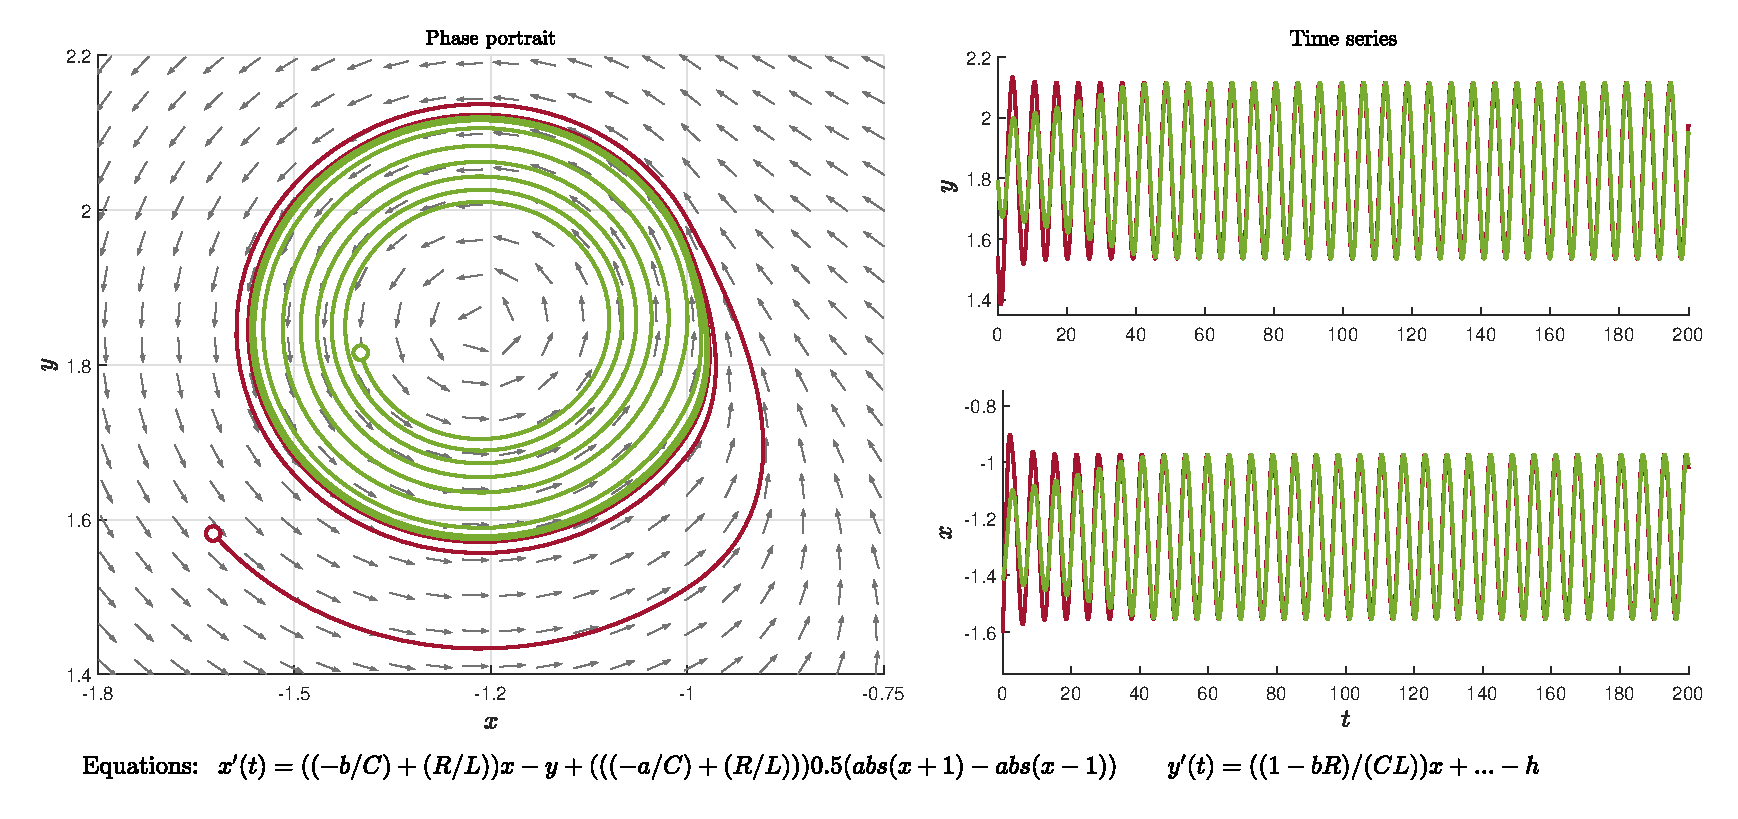
\includegraphics[width=1\textwidth]{r1.3.eps}
		\caption{Configuración de Foco Asintóticamente Inestable para $R=1.3$ donde se ha producido el Ciclo-límite debido a la bifurcación estudiada.}
		\label{fig:r1.3}
	\end{figure}\smallskip
	
	Como se puede ver hemos obtenido en nuestro circuito el mismo comportamiento que el visto en las \fref{fig:foco3}, \fref{fig:centro2}, \fref{fig:ciclolimite3}. De hecho esas figuras se representaron con la recta de separación en $x=-1$ ya que eso es lo que ocurre en nuestro circuito. Podemos comprobar que el Ciclo-Límite efectivamente se ``cuela'' levemente en la zona derecha de la recta de separación $x=-1$, ver \fref{fig:r1.3}.
	
	\vspace{0.5cm} Vamos a utilizar la función \textit{ode45} de MATLAB para solucionar el sistema de ecuaciones diferenciales \eref{eq:clejemsis} que hemos usado para las representaciones de las \fref{fig:r0.7}, \fref{fig:r1}, \fref{fig:r1.3}. Así podremos comparar los resultados que obtengamos con los que obtuvimos previamente mediante los desarrollos en series. La función \textit{ode45} tiene una herramienta muy útil para nuestro análisis ya que nos permite definir ``eventos'', en concreto estableceremos que cuando la curva solución corte a la recta $x=-1$ nos guarde el valor correspondiente de $y$, aparte del instante temporal en que se ha producido dicho evento. De esa forma podremos comprobar los puntos $y_0$ e $y_1$ además del periodo. Dejaremos que la función \textit{ode45} resuelva el sistema para un valor de tiempo grande, así nos aseguraremos que los últimos valores de $y$ que cortan a al recta $x=-1$ ya están dentro del Ciclo-Límite. En la siguiente página presentaremos el código de MATLAB utilizado para ello.
	
	\newpage
	
	\lstinputlisting[style=Matlab-editor]{Ejemplo_6.m}
	
	\vspace{0.5cm}\noindent Funciones usadas en ``Ejemplo 6'':
	\vspace{0.5cm}\lstinputlisting[style=Matlab-editor]{sistema.m}
	\vspace{0.5cm}\lstinputlisting[style=Matlab-editor]{EF.m}
	
	\newpage
	
	Como se ve en ``Ejemplo 6'' se ha establecido el punto inicial en $(-1,1)$, esto realmente no nos importa ya que nuestro sistema con $R>1$ tiene una configuración de Ciclo-Límite Asintóticamente Estable por lo que con el tiempo de studio sufuciente la solución finalmente tenderá al Ciclo-Límite. 
	
	\vspace{0.5cm}\noindent Primero vamos a obtener los últimos valores de la matriz xE ya que contendrán los últimos valores de $y_0$ e $y_1$ que cortan a la recta $x=-1$, sin olvidarnos de deshacer los cambios de variable \eref{eq:cambioo1} y \eref{eq:cambioo2} que hicimos previamente.
	
	\vspace{1cm}\lstinputlisting[style=Matlab-bw]{cw1ejem6.m}
	
	\vspace{1cm}\noindent Se han obtenido unos valores de $Y_0=0.0731$ e $Y_1=-0.1916$ muy parecidos a los obtenidos en ``Ejemplo 4'' que eran $Y_0=0.1107$ e $Y_1=-0.1694$.
	
	\newpage
	
	\vspace{0.5cm}A continuación comprobemos el periodo
	
	\vspace{1cm}\lstinputlisting[style=Matlab-bw]{cw2ejem6.m}
	
	\vspace{1cm}\noindent Hemos obtenido un periodo de $T_P=6.3797$, realmente parecido al obtenido en ``Ejemplo 4'' que era $T_P=6.4072$.
	
    \vspace{1cm}En las siguientes páginas veremos algunas gráficas interesantes que podemos obtener con los resultados de ``Ejemplo 6''
    
    \newpage
    
    	\begin{figure}[h]
    	\centering
    	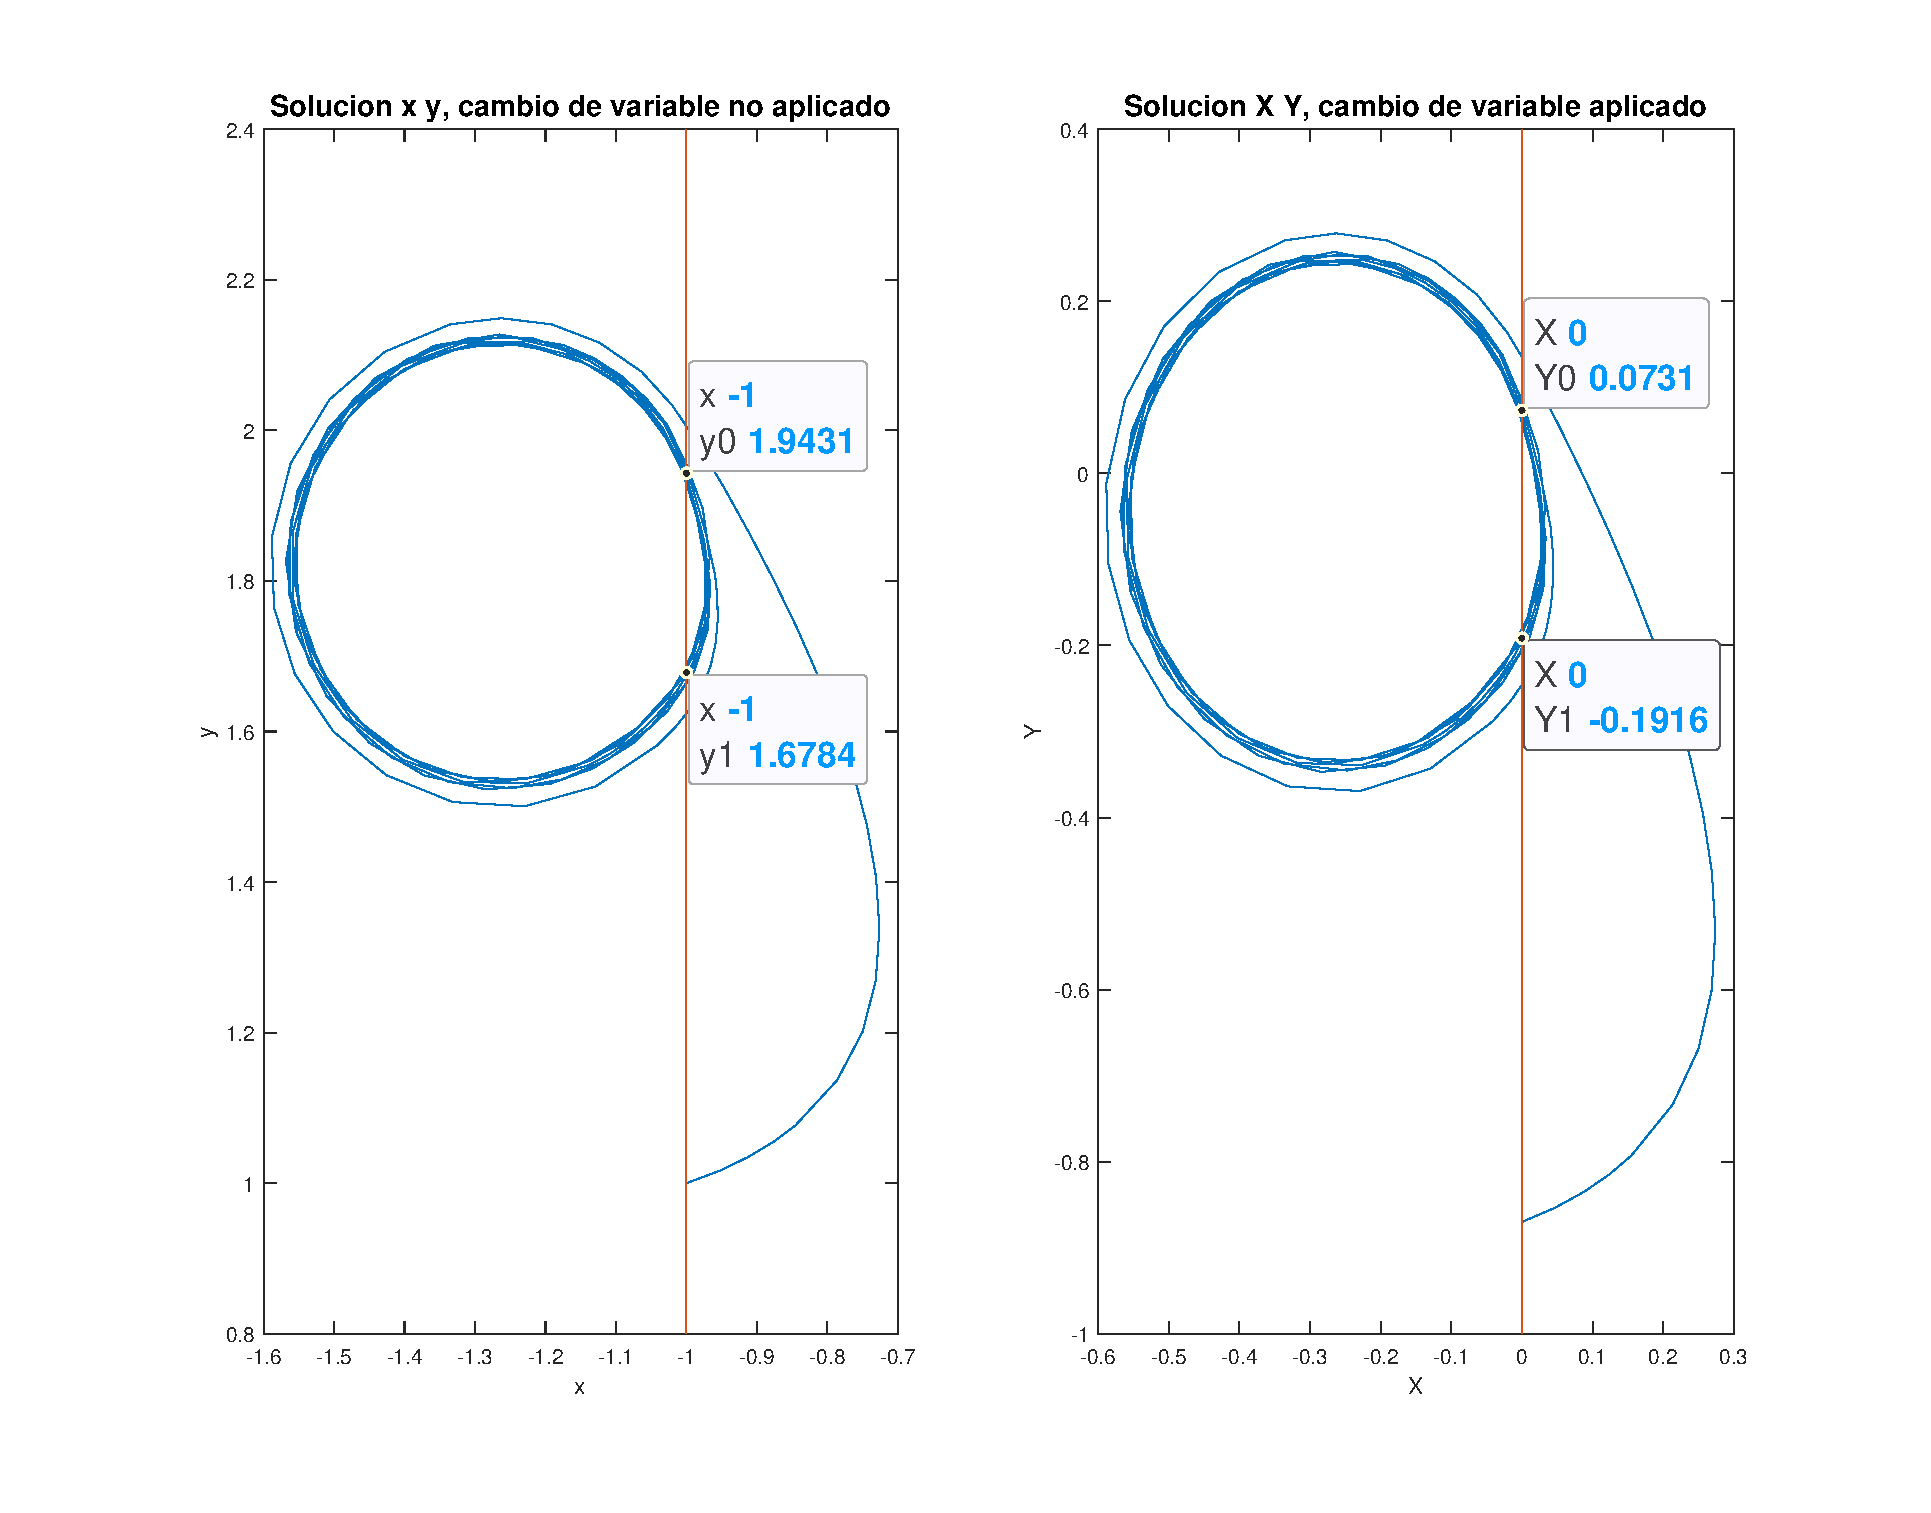
\includegraphics[width=1\textwidth]{g1ejem6.eps}
    	\caption{Comparación de la representación de la matriz \textbf{xy} de ``Ejemplo 6'' con el cambio de variable aplicado y no aplicado. Los puntos representados corresponden a las dos últimas componentes de \textbf{xE}, nuevamente con cambio de variable aplicado y no aplicado.}
    	\label{fig:g1ejem6}
    \end{figure}\smallskip
    
    \newpage
    
    \begin{figure}[h]
    	\centering
    	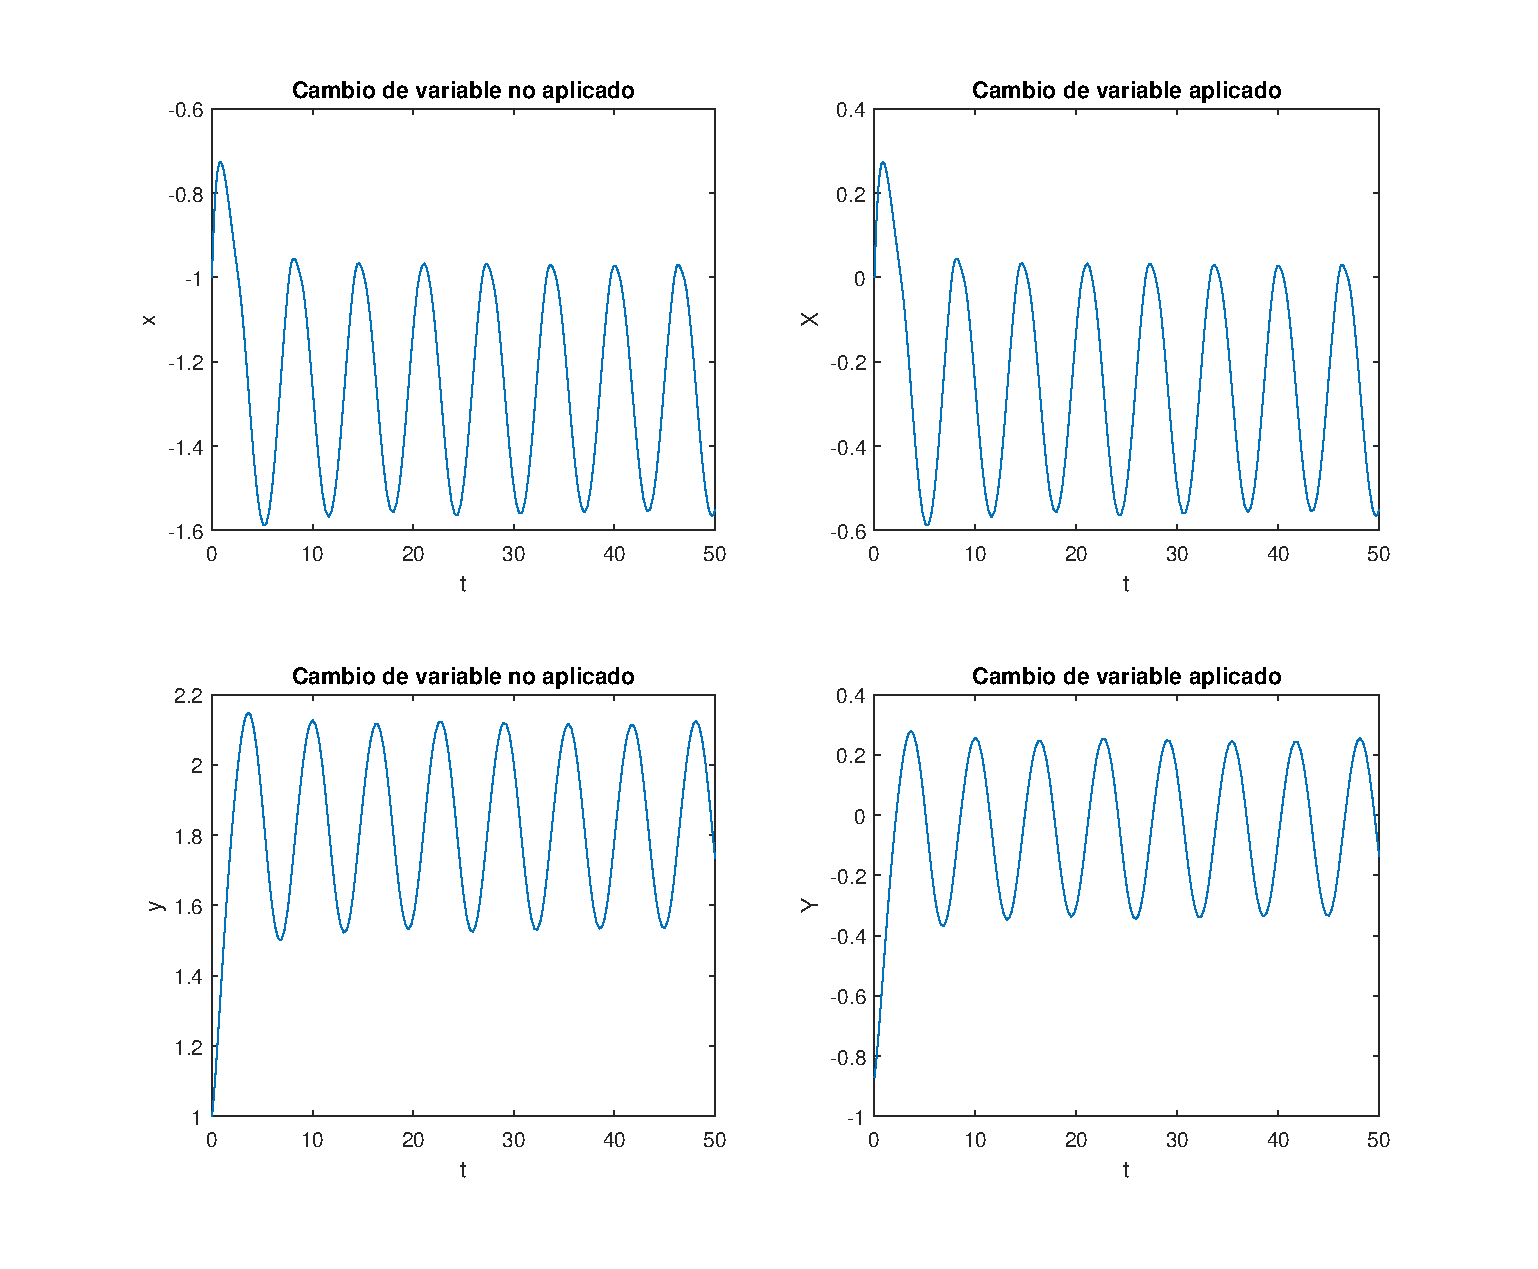
\includegraphics[width=1\textwidth]{g2ejem6.eps}
    	\caption{Comparación de la representación de las componentes de la matriz \textbf{xy} de ``Ejemplo 6'' con respecto al tiempo de estudio \textbf{t} con el cambio de variable aplicado y no aplicado.}
    	\label{fig:g2ejem6}
    \end{figure}\smallskip
	
	
	\newpage
	
	\begin{figure}[h]
		\centering
		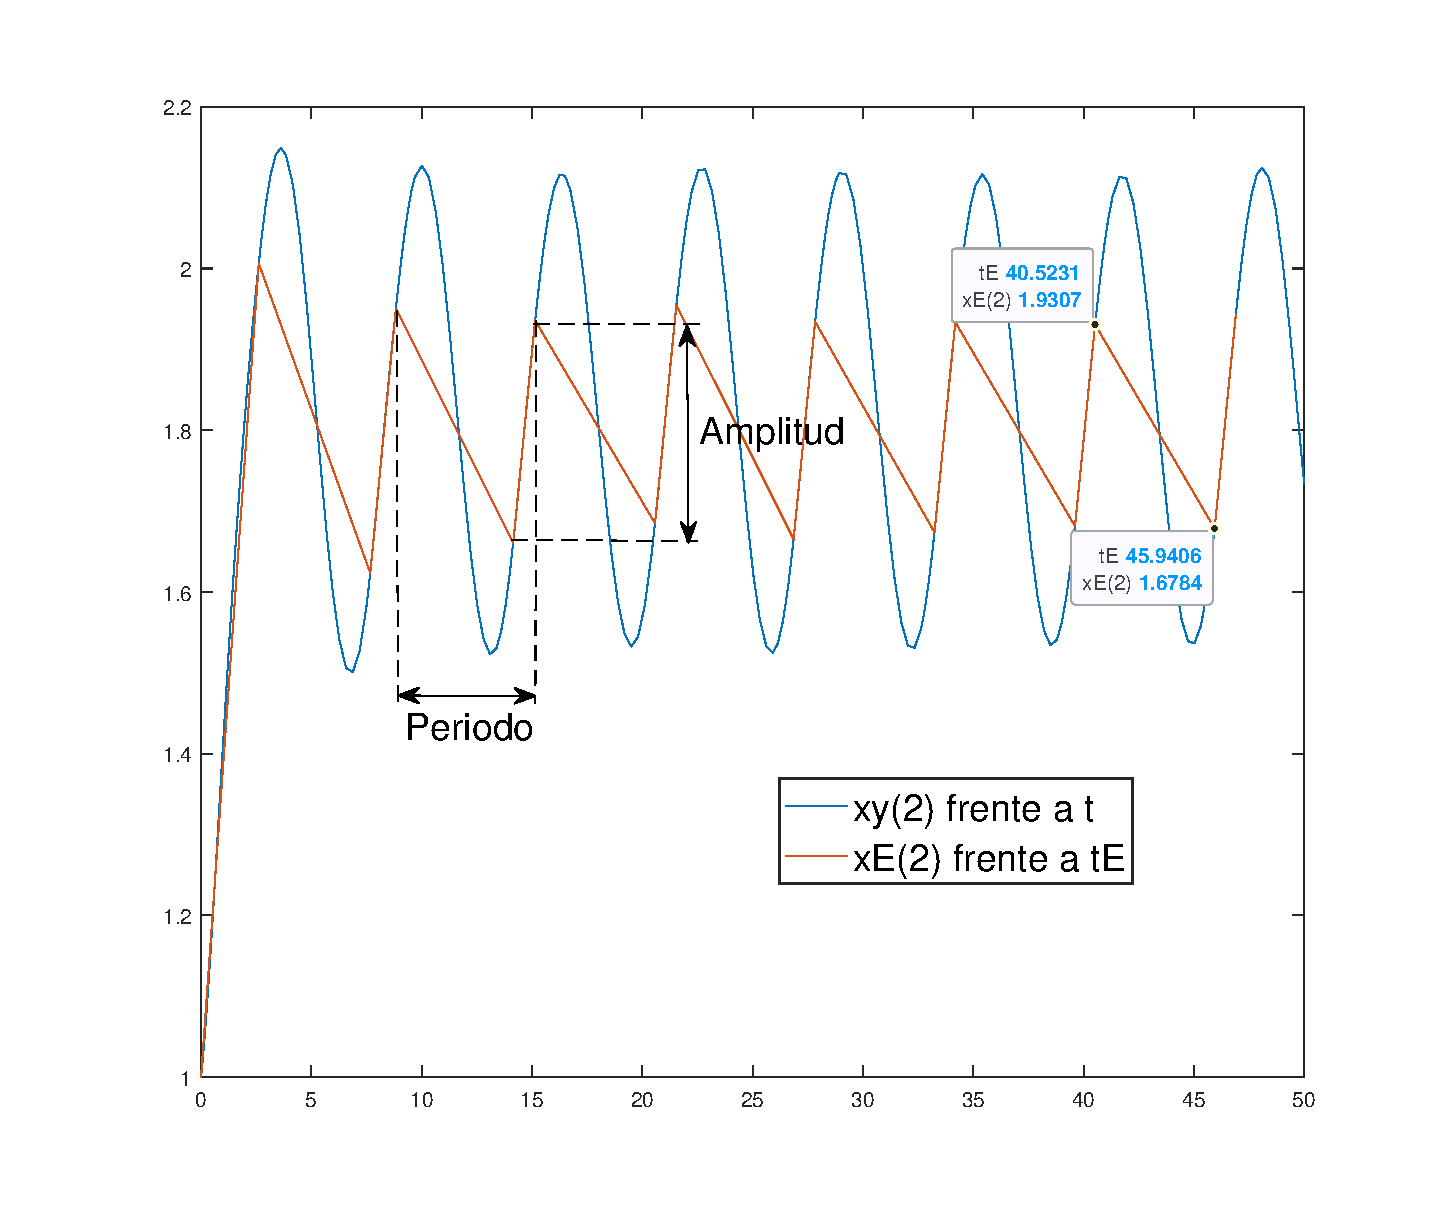
\includegraphics[width=1\textwidth]{g3ejem6.eps}
		\caption{Comparación de las gráficas de \textbf{y (xy(2))} solución frente al tiempo de estudio \textit{\textbf{t}} y los valores de \textbf{y (xE(2))} para los que se produce el evento de corte con la recta $x=-1$ frente a los instantes de tiempo \textbf{tE} en que se produce el evento. Esta gráfica es muy interesante ya que se ven muy claramente cuales son los puntos de corte $y_0$ e $y_1$ y como medir el periodo de la oscilación}
		\label{fig:g3ejem6}
	\end{figure}\smallskip
	
	\chapter*{Conclusiones}
	Contenido del capítulo de conclusiones.
	\vspace{5cm}
	\begin{equation}
		Dopado \quad No 
	\end{equation}
	
	\newpage
	
	
	\begin{thebibliography}{99}
		\bibitem{chuamissing1971} CHUA, L. O. Memristor – The missing circuit element. IEEE
		Transactions on Circuit Theory, 1971, vol. CT-18, no. 5, p. 507 to
		519. DOI: 10.1109/TCT.1971.1083337.
		
		\bibitem{chuaoscillator2008} Itoh, Makoto \& Chua, Leon. (2008). Memristor oscillators. I. J. Bifurcation and Chaos. 18. 3183-3206. 10.1142/S0218127408022354. 
		
		\bibitem{HP} Strukov DB, Snider GS, Stewart DR, Williams RS. The missing memristor found. Nature. 2008 May 1;453(7191):80-3. doi: 10.1038/nature06932. Erratum in: Nature. 2009 Jun 25;459(7250):1154. PMID: 18451858.
		
		\bibitem{williams} R. S. Williams, "How We Found The Missing Memristor," in IEEE Spectrum, vol. 45, no. 12, pp. 28-35, Dec. 2008, doi: 10.1109/MSPEC.2008.4687366.
		
		\bibitem{2021} Xiaoyue, Ji \& Dong, Zhekang \& Zhou, Guangdong \& Lai, Chun Sing \& Yan, Yunfeng \& Qi, Donglian. (2021). Memristive System Based Image Processing Technology: A Review and Perspective. Electronics. 10. 3176. 10.3390/electronics10243176. 
		
		\bibitem{outsiders} Caravelli, F. \& Carbajal, Juan. (2018). Memristors for the Curious Outsiders. 10.31224/osf.io/c4qr9. 
		
		\bibitem{teruel} Llibre, Jaume \& Teruel, Antonio. (2014). Introduction to the Qualitative Theory of Differential Systems: Planar, Symmetric and Continuous Piecewise Linear Systems. 10.1007/978-3-0348-0657-2. 
		
		\bibitem{docvic} Carmona, V.Bifurcaciones en Sistemas Dinámicos Lineales a Trozos. Tesis Doctoral. Universisdad de Sevilla, 2002.
		
		\bibitem{onsimplyfing} V. Carmona, E. Freire, E. Ponce and F. Torres, "On simplifying and classifying piecewise-linear systems," in IEEE Transactions on Circuits and Systems I: Fundamental Theory and Applications, vol. 49, no. 5, pp. 609-620, May 2002, doi: 10.1109/TCSI.2002.1001950.
		
		\bibitem{ponce} Amador, A., Freire, E., Ponce, E., and Ros, J., “On Discontinuous Piecewise Linear Models for Memristor Oscillators”, <i>International Journal of Bifurcation and Chaos</i>, vol. 27, no. 6, 2017. doi:10.1142/S0218127417300221.
		
		\bibitem{properties} Carmona, Victoriano, Fernández-Sánchez, Fernando, García-Medina, Elisabeth and Novaes, Douglas D.: Properties of Poincaré half-maps for planar linear systems and some direct applications to periodic orbits of piecewise systems, Electron. J. Qual. Theory Differ. Equ. 2023, No. 22, 1-18. doi: https://doi.org/10.14232/ejqtde.2023.1.22
		
		\bibitem{unicidad} Victoriano Carmona, Fernando Fernández-Sánchez, Douglas D. Novaes,
		Uniqueness and stability of limit cycles in planar piecewise linear differential systems without sliding region,
		Communications in Nonlinear Science and Numerical Simulation,
		Volume 123, 2023, 107257, ISSN 1007-5704.
		doi: https://doi.org/10.1016/j.cnsns.2023.107257.
		
		\bibitem{caracterizacion} Victoriano Carmona, Fernando Fernández-Sánchez,
		Integral characterization for Poincaré half-maps in planar linear systems, Journal of Differential Equations, Volume 305, 2021, Pages 319-346, ISSN 0022-0396, doi: https://doi.org/10.1016/j.jde.2021.10.010.
		
		\bibitem{ciclolimite} Ponce, E., Ros, J., Vela, E. (2013). The Focus-Center-Limit Cycle Bifurcation in Discontinuous Planar Piecewise Linear Systems Without Sliding. In: Ibáñez, S., Pérez del Río, J., Pumariño, A., Rodríguez, J. (eds) Progress and Challenges in Dynamical Systems. Springer Proceedings in Mathematics \& Statistics, vol 54. Springer, Berlin, Heidelberg. https://doi.org/10.1007/978-3-642-38830-9\_21
		
		\bibitem{amarillo} Ponce, Enrique \& Ros, Javier \& Vela, Elísabet. (2022). Bifurcations in Continuous Piecewise Linear Differential Systems: Applications to Low-Dimensional Electronic Oscillators. 10.1007/978-3-031-21135-5. 
		
		\bibitem{pv} Bachmann, K.-.-H. (1977), Henrici, P., Applied and Computational Complex Analysis, Bd. I, 682 S., New York-London-Sydney-Toronto. John Wiley \& sons. 1974. £ 13,50 .. Z. angew. Math. Mech., 57: 352-352. https://doi.org/10.1002/zamm.19770570622
		
	\end{thebibliography}
	
	\newpage
	
\end{document}
